\documentclass{jsarticle}

\title{Rust の最初のステップ}

\begin{document}
\maketitle

利用が広がり人気が高まっている新しいプログラミング言語の習得に関心がありますか? ここから始めましょう。 Rust で高速で効果的なプログラムを構築するために必要な知識の基盤を築きましょう。

このラーニング パスの内容は次のとおりです。

\begin{itemize}
\item Rust コードの最初の行を記述するために必要なツールをインストールする。
\item Rust の基本的な概念を学ぶ。
\item エラーを処理する方法を学ぶ。
\item Rust でメモリを管理する。
\item ジェネリック型と特性を使用する。
\item パッケージとクレート用のモジュールを設定する。
\item 自動テストを記述して実行する。
\item コマンドライン プログラムを作成する。
\end{itemize}

\section{Rust とは}

Rust 言語の機能、および Rust と他のプログラミング言語との比較について概要を簡単に説明します。

\subsection{はじめに}

Rust プログラミング言語を使用すると、信頼性と効率性に優れたシステム ソフトウェアをビルドできます。 開発者は、Web サーバー、メール サーバー、Web ブラウザーなどのネットワーク ソフトウェアに Rust を使用します。 Rust は、コンパイラとインタープリター、仮想化とソフトウェア コンテナー、データベース、オペレーティング システム、および暗号化にも存在します。 Rust を使用して、組み込みデバイス用のゲーム、コマンドライン プログラム、Web アセンブリ プログラム、アプリケーションをビルドできます。

Rust は、C や C++ などの既存のシステム ソフトウェア言語の安全な代替手段です。 C や C++ と同様に、Rust には大規模なランタイムまたはガベージ コレクターが "ありません"。これは、他のほとんどすべての新しい言語とは対照的です。 ただし、C や C++ とは異なり、Rust ではメモリの安全性が保証されています。 Rust を使用すると、C や C++ で発生する可能性のあるメモリの誤用に関連するバグの多くを防ぐことができます。

Rust では、パフォーマンス、安全性、および実装の表現が独自のバランスを保っています。 どのようなプログラミング歴でも、Rust には何かしら役立つ機能があります。

\subsubsection{Rust を学習する最善の方法}

Rust を使用する場合、Rust コードを生産的に記述できるようになるには、理論的な知識が少し必要です。 開発を開始するには、まず、このコースや他の Rust の学習用リソースを理解する必要があります。 言語の基本的な知識を習得したら、可能な限りコードの記述を練習します。 このモジュールの演習と、このラーニング パスの他の演習を実践します。

まず、言語の小規模で基本的な概念について学習します。 次に、演習と探索によって基礎を構築します。 途中でいくつかのプロジェクトを作成し、このレッスンが終わるまでにその言語をしっかり理解します。

\subsubsection{学習の目的}

このモジュールでは、次のことを学習します。

\begin{itemize}
\item いくつかの Rust 固有の機能
\item 開発者が他のプログラミング言語ではなく Rust を選ぶ理由
\item Rust プログラムをビルド、コンパイル、実行するための基本的なコンポーネントとツール
\item Rust プレイグラウンドを試す
\end{itemize}
 % はじめに
\subsection{Rust とは}

Rust は、効率的で安全なソフトウェアの開発に使用できるオープンソースのシステム プログラミング言語です。 Rust を使用すると、メモリを管理し、その他の低レベルの詳細を制御できます。 ただし、イテレーションやインターフェイスなど、高レベルの概念も活用できます。 こうした機能が Rust と、C や C++ のような低レベル言語との違いになります。

さらに、Rust には、幅広いアプリケーションで使用することを可能にする次のような利点があります。

\begin{itemize}
\item \textbf{タイプ セーフ}: コンパイラによって、型が間違っている変数に操作が適用されないことが保証されます。
\item \textbf{メモリ セーフ}: Rust ポインター ("参照" と呼ばれます) によって、常に有効なメモリが参照されます。
\item \textbf{データ競合なし}: プログラムの複数の部分が同時に同じ値を変化させることができないようにする Rust のボロー チェッカーによって、スレッドセーフが保証されます。
\item \textbf{ゼロコスト抽象化}: Rust では、イテレーションやインターフェイス、関数型プログラミングなどの高度な概念を、パフォーマンス コストをほとんど、またはまったくかけずに利用できます。 抽象化は、基になるコードを手動で記述した場合と同様に実行されます。
\item \textbf{最小限のランタイム}: Rust のランタイムはごく小さく、省略可能です。 この言語には、メモリを効率的に管理するためのガベージ コレクターもありません。 このように、Rust は C や C++ などの言語とよく似ています。
\item \textbf{ターゲットはベアメタル}: Rust では、組み込みの "ベアメタル" プログラミングをターゲットにすることができます。これにより、オペレーティング システムのカーネルまたはデバイス ドライバーを記述するのに適しています。
\end{itemize}

2021 年の Stack Overflow による開発者アンケートによれば、Rust は、数年連続で最も好まれている言語になっています。 開発者は Rust を使用してプログラミングを楽しんでいます。 スタートアップ企業から大企業まで、さまざまな種類の組織が独自の用途に Rust を使用しています。 ツールの構築から Web アプリの作成、サーバーでの作業、組み込みシステムの作成に至るまで、その可能性は無限です。 % Rust とは
\subsection{Rust 固有の機能}

あるプログラミング言語がプロジェクトに適しているかどうかを判断するには、その機能と制限事項を知る必要があります。 そのうえで、候補となる言語を比較し、最適な言語を選択できます。

このレッスンでは、Rust の機能と制限事項のうち、いくつかを検討します。

\begin{itemize}
\item Rust モジュール システム: モジュール、クレート、パス
\item Rust 標準ライブラリとサードパーティ製のクレート
\item Rust の Cargo ツールと依存関係マネージャー
\item Rust を使用するケース
\end{itemize}

\subsubsection{Rust モジュール システムを使用してコードを管理する}

Rust には、コードの管理と整理に役立つ機能のコレクションが用意されています。 これらの機能は、"Rust モジュール システム" と呼ばれます。 システムは、クレート、モジュール、パス、およびそれらの項目を操作するためのツールで構成されます。

\begin{itemize}
\item \textbf{クレート}: Rust クレートはコンパイル単位です。 これは、Rust コンパイラで実行できる最小のコード単位です。 クレート内のコードはまとめてコンパイルされ、バイナリ実行可能ファイルまたはライブラリが作成されます。 Rust では、クレートだけが再利用可能な単位としてコンパイルされます。 クレートには、最上位に暗黙的で名前のないモジュールがある、Rust モジュールの階層が含まれています。

\item \textbf{モジュール}: Rust モジュールは、クレート内の個々のコード項目のスコープを管理できるようにすることで、プログラムを整理しやすくします。 関連するコード項目または一緒に使用される項目は、同じモジュールにグループ化することができます。 再帰コード定義は、他のモジュールにまたがることができます。

\item \textbf{パス}: Rust では、パスを使用してコード内の項目に名前を付けることができます。 たとえば、パスとして、ベクター、コード関数、場合によってはモジュールといったデータ定義が考えられます。 また、モジュール機能はパスのプライバシーの制御にも役立ちます。 公開でアクセスできるコードの部分と非公開の部分を指定できます。 この機能を使用すると、実装の詳細を隠すことができます。
\end{itemize}

\subsubsection{Rust のクレートとライブラリを使用する}

Rust 標準ライブラリ \texttt{std} には、Rust プログラムの基本的な定義と操作のための再利用可能なコードが含まれています。 このライブラリには、\texttt{String} や \texttt{Vec<T>} のようなコア データ型の定義、Rust プリミティブの操作、一般的に使用されるマクロ関数のコード、入出力アクションのサポート、およびその他多くの分野の機能が含まれています。

Rust プログラムで使用できるライブラリとサードパーティ製のクレートは何万種類もあり、そのほとんどが、Rust のサードパーティ製のクレート リポジトリ crates.io からアクセスできます。 これらのクレートにプロジェクトからアクセスする方法については後ほど学習しますが、ここではプログラミング演習で使用するクレートをいくつか紹介します。

\begin{itemize}
\item std - Rust 標準ライブラリ。 Rust の演習では、次のモジュールを確認します。
\begin{itemize}
\item std::collections - コレクション型の定義。HashMap など。
\item std::env - お使いの環境を操作する関数。
\item std::fmt - 出力形式を制御する機能。
\item std::fs - ファイル システムを操作する関数。
\item std::io - 入力/出力を操作する定義と機能。
\item std::path - ファイル システム パス データの操作をサポートする定義と関数。
\end{itemize}
\item structopt - コマンド ライン引数を簡単に解析するためのサードパーティ製のクレート。
\item chrono - 日付と時刻のデータを処理するサードパーティ製のクレート。
\item regex - 正規表現を処理するサードパーティ製のクレート。
\item serde - Rust データ構造のシリアル化および逆シリアル化操作のサードパーティ製のクレート。
\end{itemize}


既定では、\texttt{std} ライブラリは、すべての Rust クレートで使用できます。 クレートまたはライブラリ内の再利用可能コードにアクセスするために、\texttt{use} キーワードが実装されています。 \texttt{use} キーワードを使用すると、クレートまたはライブラリ内のコードが "スコープに取り込まれる" ので、プログラム内で定義と関数にアクセスできます。 標準ライブラリには、\texttt{use std::fmt} のように、パス \texttt{std} を含む \texttt{use} ステートメントでアクセスします。 その他のクレートまたはライブラリには、\texttt{use regex::Regex} のように、それらの名前でアクセスします。

\subsubsection{Cargo を使用してプロジェクトを作成して管理する}

Rust コンパイラ (\texttt{rustc}) を直接使用してクレートをビルドすることもできますが、ほとんどのプロジェクトは、Cargo と呼ばれる Rust ビルド ツール兼依存関係マネージャーを使用しています。

Cargo は、次のような多くの機能を備えています。

\begin{itemize}
\item \texttt{cargo new} コマンドを使用して、新しいプロジェクト テンプレートを作成する。
\item \texttt{cargo build} コマンドを使用して、プロジェクトをビルドする。
\item \texttt{cargo run} コマンドを使用して、プロジェクトをビルドして実行する。
\item \texttt{cargo test} コマンドを使用して、プロジェクトをテストする。
\item \texttt{cargo check} コマンドを使用して、プロジェクトの種類を確認する。
\item \texttt{cargo doc} コマンドを使用して、プロジェクトのドキュメントをビルドする。
\item \texttt{cargo publish} コマンドを使用して、crates.io にライブラリを発行する。
\item Cargo.toml ファイルにクレート名を追加して、依存クレートをプロジェクトに追加する。
\end{itemize}

\subsubsection{Rust を使用するケース}

Rust 言語には、プロジェクトに最適な言語を選択する際に考慮すべき多くの長所があります。

\begin{itemize}
\item Rust を使用すると、この言語で記述されたプログラムやライブラリのパフォーマンスとリソースの消費量を C および C++ と同等に制御できますが、既定でメモリ セーフであるため、よくあるバグの種類全体が排除されます。
\item Rust には豊富な抽象化機能が備わっているので、開発者はプログラムの不変条件の多くをコードにエンコードしてから、慣習やドキュメントに頼ることなくコンパイラでチェックできます。 この機能により、"コンパイルできれば動作する" と感じるようになることも多くあります。
\item Rust には、コードのビルド、テスト、文書化、共有を行うためのツールが組み込まれています。また、サードパーティ製のツールやライブラリの豊富なエコシステムも整っています。 これらのツールを使用すると、一部の言語では依存関係の構築などの難しい作業を、Rust では簡単かつ生産性の高い方法で行うことができます。
\end{itemize}

\subsubsection{自分の知識をチェックする}

\begin{enumerate}
\item Rust を使用することの説得力のある強みは何ですか?
\begin{itemize}
\item Rust は、タイプセーフ、メモリ セーフであり、データの競合がありません。
\item Rust は、オペレーティング システムなどベアメタル開発に最適化されています。
\item Rust にはメモリを効率的に管理できる、堅牢なガベージ コレクターがあります。
\end{itemize}
\item Rust コードはどのように実行されますか?
\begin{itemize}
\item Rust によってスクリプトが解釈される。
\item C/C++ ソース ファイルに Rust コードを含める必要がある。
\item コンパイル後に直接実行される。
\end{itemize}
\item Cargo で できないこと の例はどれですか?
\begin{itemize}
\item 既存の Rust プロジェクトをビルドする。
\item インストールされている Rust コンパイラのバージョンを更新する。
\item ライブラリを Crates.io に発行する。
\end{itemize}
\end{enumerate}







 % Rust 固有の機能
\subsection{Rust プレイグラウンド}

少しの Rust コードを試したり、Rust ライブラリ内の定義の構文を確認したりしたい場合があります。 また、何らかのコードを他のユーザーとすばやく共有する必要がある場合もあります。 Rust 言語では、Rust プレイグラウンドでこれらのタスクに対するサポートが用意されています。

プレイグラウンドは、インターネット上 (\texttt{https://play.rust-lang.org/}) で利用できる Rust 開発用の IDE です。 プレイグラウンドには誰でもアクセスできます。 コードを記述した後、同じ環境でコードをコンパイルして実行できます。 次のスクリーンショットは、プレイグラウンド環境を示しています。 ツール バーの右端にある [構成] メニューには、環境の設定を行うオプションがあります。

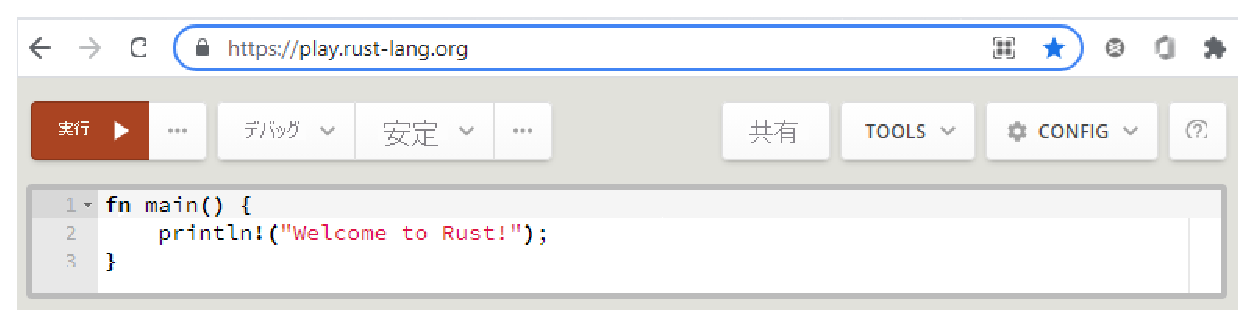
\includegraphics[width=14cm]{rust-playground-main.eps}

プレイグラウンドでは、Rust \texttt{std} 標準ライブラリのメソッドと関数にアクセスできます。 crates.io ライブラリで最もダウンロードされている上位 100 のクレートも、それらの依存関係と共に使用できます。

\subsubsection{ツールと機能}

Rust プレイグラウンドには、組み込みのツールと開発機能がいくつか用意されています。

\begin{itemize}
\item 書式コード: Rustfmt ツールを使用すると、公式の Rust スタイルを使用するようにコードを書式設定できます。 このツールによってコードが調整され、要素と演算子の間に推奨されているインデントと間隔が適用されます。
\item テスト コード: Clippy ツールでは、コード内に誤りがないかどうか確認します。 このツールでは、コードに対して lint テストを実行し、エラーや改善する領域を見つけることができます。
\item コードの保存: Rust プレイグラウンドでの作業時に、そのコードがブラウザーのローカル ストレージに自動的に保存されます。 この機能により、特にブラウザー ウィンドウを偶然閉じてしまった場合に、最新の作業を簡単に復旧できます。
\item コードの共有: [共有] 機能により、プレイグラウンド内のコード用に共有可能な GitHub gist が作成されます。 この URL を保存することで、後でコードにアクセスできます。 URL によって、特定のコードの gist がプレイグラウンドに読み込まれます。
\end{itemize}

\begin{itembox}[l]{注意}
ブラウザーのローカル ストレージは、シングルトン リソースです。 複数のブラウザー ウィンドウで Rust プレイグラウンドを開き、各ウィンドウで異なるコードを操作している場合、すべてのウィンドウの中で最後に保存されたコードだけがローカル ストレージに保持されます。
\end{itembox}

\subsubsection{ビルド オプション}

Rust プレイグラウンドには、コードをビルドして実行するためのいくつかのオプションがあります。

\begin{itemize}
\item \textbf{Run}: コードをビルドして実行し、出力を表示します。 [Run] オプションは、 コマンドを使用することと同じです。
\item \textbf{Build}: コードをビルドしますが、そのコードは実行しません。 [Build] オプションは、 コマンドを使用することと同じです。
\item \textbf{Test}: コードをビルドし、そのコードに対してすべてのテストを実行します。 [Test] オプションは、 コマンドを使用することと同じです。
\end{itemize}

\subsubsection{保護の制限}

プレイグラウンドには、サイトが不正な手段で使用されるのを防ぐ制限事項が設けられています。 この制限事項により、すべてのユーザーがこのサイトを使用し続けることができます。

\begin{itemize}
\item \textbf{ネットワーク}: プレイグラウンドでコードをコンパイルまたは実行するときは、ネットワーク接続を使用できません。
\item \textbf{メモリ}: プレイグラウンドでは、コードをコンパイルしてビルドされたプログラムを実行するために使用できるメモリが制限されます。
\item \textbf{実行時間}: プレイグラウンドでは、コードをコンパイルしてビルドされたプログラムを実行する最大時間が設定されています。
\item \textbf{ディスク}: コードをコンパイルしてビルドされたプログラムを実行するために使用できるディスク領域の量は制限されています。
\end{itemize}



Rust プレイグラウンドの機能の詳細については、Rust の Web サイトを参照してください。


\subsubsection{自分の知識をチェックする}

次の質問に答えて、学習した内容を確認してください。

\begin{enumerate}
\item コードの間違いを見つけるために使用できる Rust プレイグラウンド ツールはどれですか?
\begin{itemize}
\item rustfmt
\item Clippy
\item デバッグ
\end{itemize}
\item Rust プレイグラウンドでネットワーク接続を利用できなくなるのはどのようなときですか。
\begin{itemize}
\item コードの編集中。
\item プログラムの実行中。
\item コードのコンパイル中、またはプログラムの実行中。
\end{itemize}

\end{enumerate}


 % Rust プレイグラウンド
\subsection{演習}

Rust プレイグラウンドは、小規模のプログラムをテストし、新しいクレートとライブラリを試し、他のユーザーとコードを共有する場合に便利です。 この演習では、プレイグラウンドで小規模のプログラムをビルドして、この環境について理解を深めます。

\subsubsection{プレイグラウンドでコードを記述する}

まず、基本的なプログラムのコードを記述します。

\begin{enumerate}
\item Rust playground に接続します。

\item プレイグラウンド エディターで次のコードを入力します。

\begin{lstlisting}[numbers=none]
fn main(){println!(Welcome to Rust!);}
\end{lstlisting}

\item [Tools][Rustfmt] の順に選択し、コードを書式設定します。
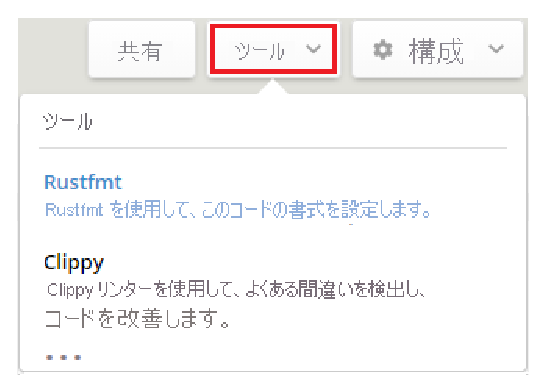
\includegraphics[width=10cm]{rust-playground-tools.eps}

このツールでは、公式の Rust スタイルを試用するようにコードを調整します。
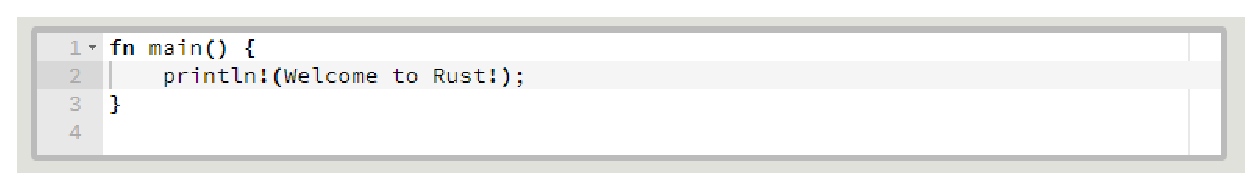
\includegraphics[width=14cm]{rust-playground-rustfmt.eps}

\item [Tools][Clippy] の順に選択して、コード内の誤りを確認します。 結果はエディターの下に表示されます。
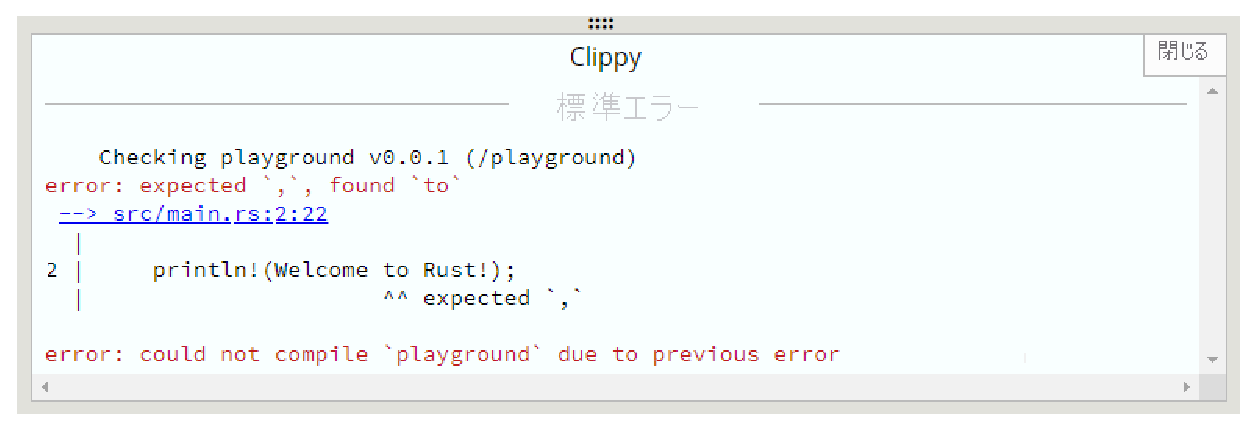
\includegraphics[width=14cm]{rust-playground-clippy.eps}

\item サンプル コードを修正するには、"Welcome to Rust!" というテキストの前後に引用符を追加します。
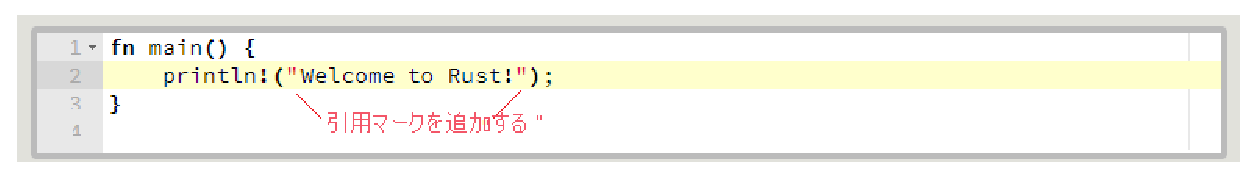
\includegraphics[width=14cm]{rust-playground-add-quotes.eps}

\end{enumerate}


\subsubsection{プレイグラウンドでコードをビルドして実行する}

次に、コードをコンパイルして、プログラムを実行します。

\begin{enumerate}
\item プレイグラウンドでコードをビルドして実行する方法を選択するには、UI の上部にある [Run] ドロップダウン メニューを開きます。

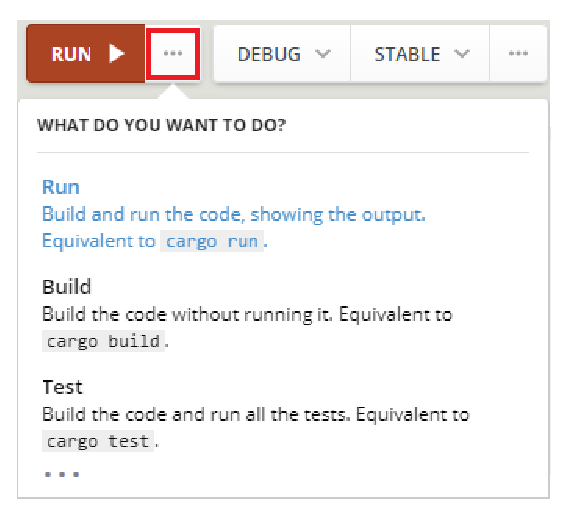
\includegraphics[width=10cm]{rust-playground-run.eps}

\item [Run] を選択して、サンプル プログラムをビルドして実行します。 プログラムの出力がエディターの下に表示されます。

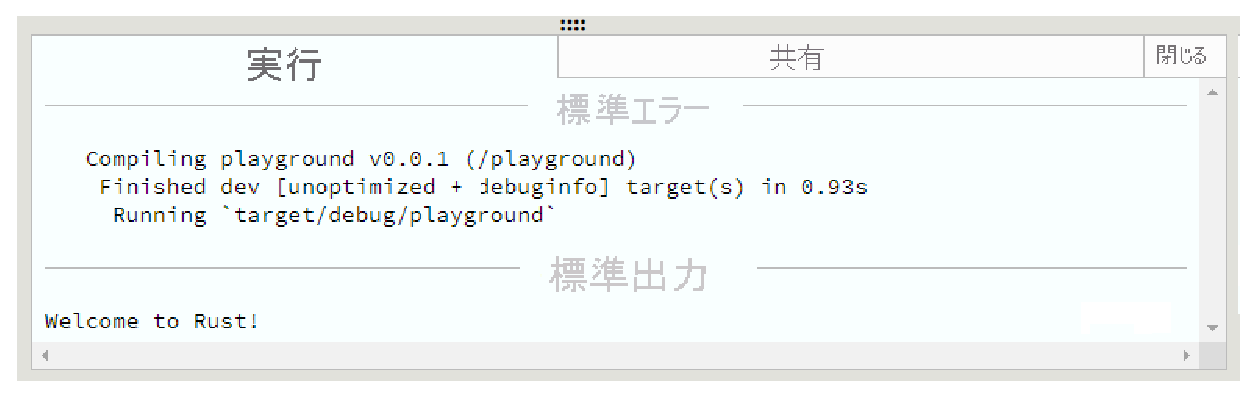
\includegraphics[width=14cm]{rust-playground-print.eps}

\end{enumerate}

\subsubsection{プレイグラウンドでコードを保存して共有する}

プレイグラウンドで作業するときに、コードはブラウザー ストレージに自動的に保存されます。 ブラウザー ウィンドウを閉じると、入力したコードが失われる場合があります。 コードを常に使用できるようにするために、共有可能な URL を作成できます。

\begin{enumerate}
\item ツール バーの [Share] 機能を選択して、プレイグラウンド内のコードの GitHub gist を作成します。

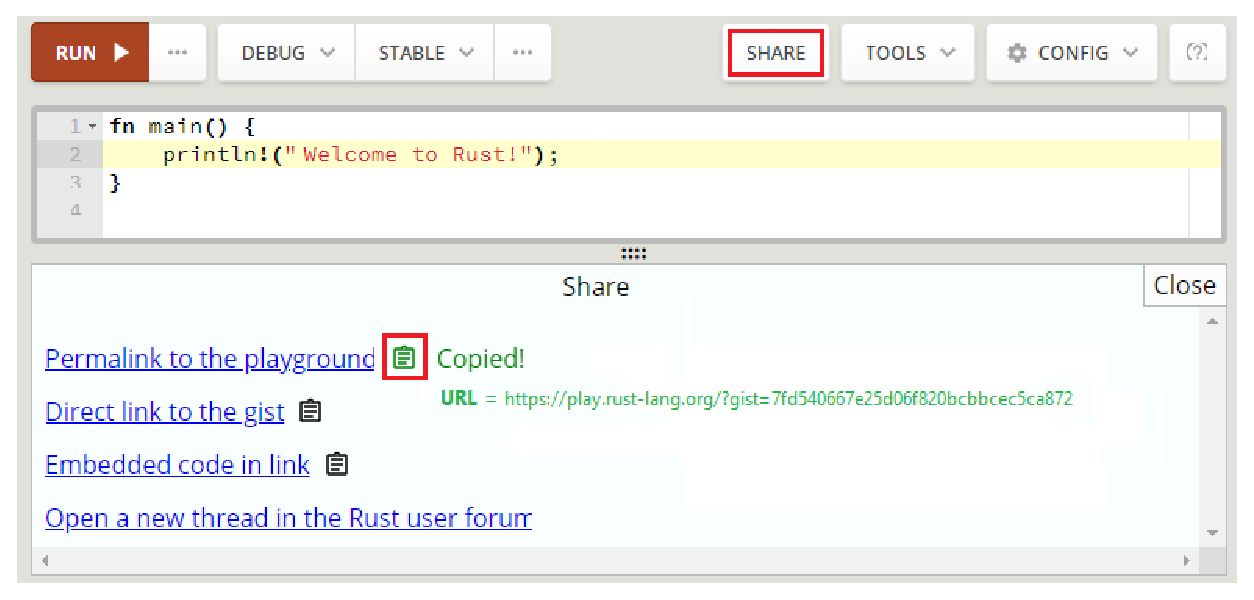
\includegraphics[width=14cm]{rust-playground-share.eps}

\item [Permalink to the playground] というテキストの横にある紙のアイコンを選択して、コードの共有可能 gist を取得します。
\end{enumerate}






 % 演習
\subsection{まとめ}


このモジュールでは、Rust プログラミング言語を使用してビルドできるアプリケーションの種類について学習しました。 Rust は低レベルと高レベルの開発の両方で有用である。

コードを操作するために Rust コマンドを確認しました。 \texttt{rustc} コマンドは、Rust プログラムを記述してコンパイルするために使用される。

Rust Cargo 機能を把握し、コード編成のためのモジュール システムについて学習しました。 新しいプロジェクトを作成し、ビルドして実行するために Cargo を使用します。

Rust プレイグラウンド環境について確認し、コードを記述、ビルド、テスト、実行する方法を学習しました。

\subsubsection{Rust クックブックのレシピを試す}

Rust クックブックには、一般的なプログラミング タスクで推奨されているプラクティスに従うコードの "レシピ" が含まれています。 レシピに従って、Rust で一般的に使用されているクレートを操作する方法を学習できます。 レシピでは、テキストと数値の処理、データベースの操作、一般的なアルゴリズムの適用、プログラムのデバッグなど、さまざまなトピックが取り上げられています。 Rust クックブックは、Rust の Web サイトで確認できます。 % まとめ





 % Rust とは
\section{Rust 開発環境を設定する}

Rust 開発環境を設定し、プログラムを記述し、Cargo ビルド システムを使用する方法について説明します。

\subsection{学習の目的}

このモジュールでは、次の方法を学習します。

\begin{itemize}
\item Rust を使用するための開発環境を設定します。
\item 単純な "Hello World" プログラムを 作成します。
\item Rust のビルド ツールであり、依存関係マネージャーである Cargo を使用します。
\end{itemize}



\subsection{はじめに}

このユニットでは、Rust でのプログラミングを開始できるよう、開発環境をインストールして構成する手順について説明します。

Rust でプログラミングするには、Visual Studio Code エディター、Visual Studio Code 用 Microsoft C++ ビルド ツール、Rust 言語ファイルをインストールします。

環境を設定したら、基本的な "Hello World!" プログラムを試して、 次に進む準備ができたかを確認します。

\subsubsection{学習の目的}

このモジュールでは、次の方法を学習します。

\begin{itemize}
Rust を使用するように開発環境を設定します。
基本的な "Hello World!" をコンパイルして実行します 作成します。
Rust のビルド ツールであり、依存関係マネージャーである Cargo を使用します。
\end{itemize}
 % はじめに
\subsection{Visual C++ ビルド ツールをインストールする}

Rust には、Visual Studio 2013 以降の Microsoft C++ ビルド ツールが必要です。 Rust をインストールするには、事前にこれらのビルド ツールがインストールされている必要があります。

ビルド ツールがインストールされていない場合は、次の手順に従います。


\begin{enumerate}
\item Microsoft Visual Studio Code のダウンロード ページにアクセスします。

\item $[$Build Tools のダウンロード] を選択します。

\item ダウンロードが完了したら、インストーラー ファイルを実行します。 Visual Studio インストーラー ウィンドウが開きます。

\item ポップアップ ダイアログで、[はい] を選択します。 次のポップアップ ダイアログで、[続行] を選択します。

\item インストーラー ウィンドウの [デスクトップとモバイル] で、左側にある [C++ Build Tools] オプションのチェックボックスをオンにします。

\item 右側の [インストールの詳細] ウィンドウで、次のオプションが選択されていることを確認します。
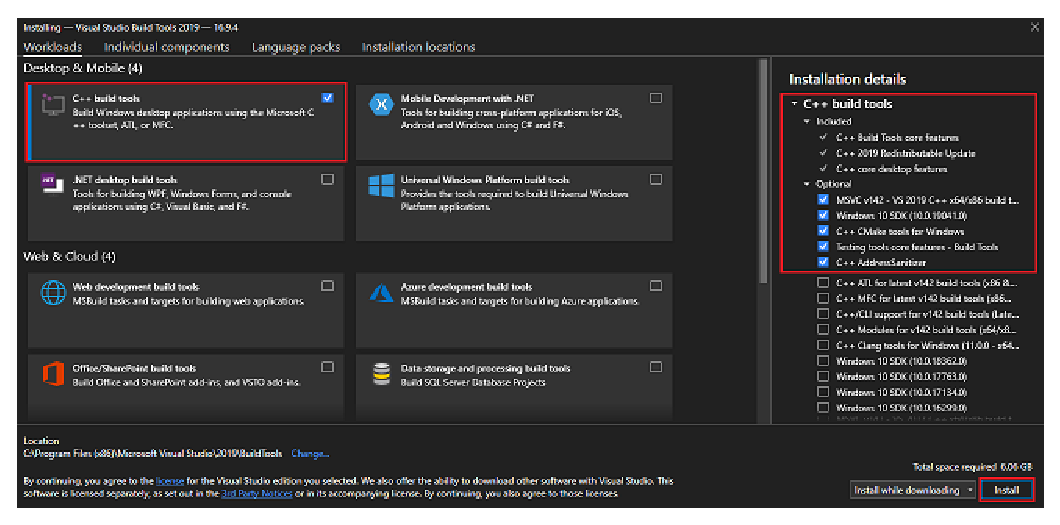
\includegraphics[width=14cm]{install-visual-cpp-build-tools.eps}

\item 右下にある [インストール] を選択します。
\end{enumerate}

インストールが完了したら、Rust のインストールを続行できます。
 % Visual Studio Code をインストールする
\subsection{Visual C++ ビルド ツールをインストールする}

Rust には、Visual Studio 2013 以降の Microsoft C++ ビルド ツールが必要です。 Rust をインストールするには、事前にこれらのビルド ツールがインストールされている必要があります。

ビルド ツールがインストールされていない場合は、次の手順に従います。


\begin{enumerate}
\item Microsoft Visual Studio Code のダウンロード ページにアクセスします。

\item $[$Build Tools のダウンロード] を選択します。

\item ダウンロードが完了したら、インストーラー ファイルを実行します。 Visual Studio インストーラー ウィンドウが開きます。

\item ポップアップ ダイアログで、[はい] を選択します。 次のポップアップ ダイアログで、[続行] を選択します。

\item インストーラー ウィンドウの [デスクトップとモバイル] で、左側にある [C++ Build Tools] オプションのチェックボックスをオンにします。

\item 右側の [インストールの詳細] ウィンドウで、次のオプションが選択されていることを確認します。
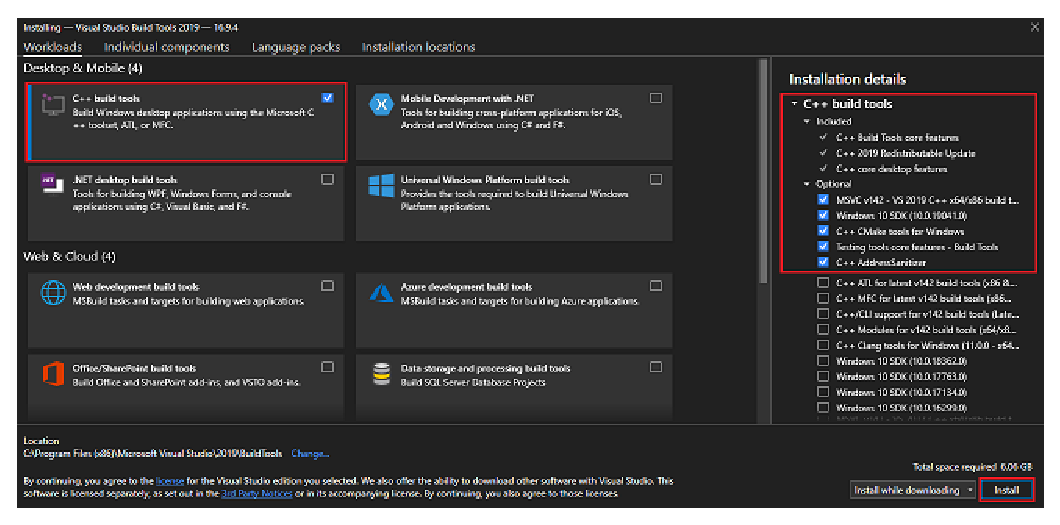
\includegraphics[width=14cm]{install-visual-cpp-build-tools.eps}

\item 右下にある [インストール] を選択します。
\end{enumerate}

インストールが完了したら、Rust のインストールを続行できます。
 % Visual C++ ビルド ツールをインストールする
\subsection{Rust をインストールする}

Rust をインストールするために推奨される方法は、Rust ツールチェーン インストーラーの \texttt{rustup} を使用することです。 Web サイト rustup.rs にアクセスして、お使いのオペレーティング システムに合った手順を見つけてください。

\includegraphics[width=10cm]{rustup.eps}

Linux または macOS 上では、クリップボード アイコンを選択して curl コマンドをコピーします。 次に、コンピューターのターミナルまたはコマンド プロンプトを開いてコマンドを貼り付け、画面の指示に従います。 Windows 上では、インストーラーの指示に従います。

\begin{itembox}[l]{重要}
Rust には、Visual Studio 2013 以降の Microsoft C++ ビルド ツールが必要です。 Rust をインストールするには、事前にビルド ツールがインストールされている必要があります。 ビルド ツールをインストールする必要がある場合は、前のユニットの手順を参照してください。
\end{itembox}

Rust のラピッド リリース プロセスは 6 週間ごとに実行されます。非常に多くのプラットフォームがサポートされているので、任意の時点で利用できる Rust のビルドは多数存在します。 \texttt{rustup} を以前にインストールしたことがある場合は、\texttt{rustup update} コマンドを実行することで、Rust の最新の安定バージョンに更新できます。

\subsubsection{Rust のインストールを確認する}

Rust のインストールを完了したら、\texttt{rustc} コマンドと \texttt{cargo} コマンドを使用できるようになります。

\begin{itembox}[l]{注意}
次のコマンドはすべてのプラットフォームで動作します。
\end{itembox}

ターミナルまたはコマンド プロンプトで、次のコマンドを実行します。


\begin{lstlisting}[numbers=none]
rustc --version
\end{lstlisting}

この例のような出力になるはずです。

\begin{lstlisting}[numbers=none]
rustc 1.50.0 (cb75ad5db 2021-02-10)
\end{lstlisting}

次に、次のコマンドを実行します。

\begin{lstlisting}[numbers=none]
cargo --version
\end{lstlisting}

次のような出力が表示されます。

\begin{lstlisting}[numbers=none]
cargo 1.50.0 (f04e7fab7 2021-02-04)
\end{lstlisting}

いずれの出力行にも、利用可能な Rust と Cargo の最新の安定したバージョンに関する次の情報が含まれます。

\begin{itemize}
\item リリース番号
\item コミット ハッシュ
\item コミットの日付
\end{itemize}

この情報は次の形式で表示されます。

\texttt{<executable-name> <three-part-release-number> (<9-character-hash-code> <4-digit-year>-<2-digit-month>-<2-digit-day>)}

この種類の出力が表示された場合、両方のインストールが成功しました。 この情報が表示されない場合、\texttt{PATH} 環境変数を確認してください。 \texttt{rustc.exe} と \texttt{cargo.exe} という実行可能ファイルが入っているフォルダーが必ず含まれるようにしてください。

\subsubsection{自分の知識をチェックする}

次の質問に答えて、学習した内容を確認してください。

\begin{enumerate}
\item Rust のインストールに使用するために推奨されているコマンドは何ですか?

\begin{itemize}
\item rinstall
\item rustup
\item rupdate
\end{itemize}

\item Rust ライブラリはどのくらいの頻度で更新されますか?
\begin{itemize}
\item 6 か月ごと
\item 3 か月ごと
\item 6 週間ごと
\end{itemize}
\end{enumerate}

 % Rust をインストールする
\subsection{演習: Hello World}

Rust がインストールされていれば、コーディングを開始する準備ができています。 "Hello, world!" を出力するプログラムを作成しましょう。 コンソールに表示します。

\subsubsection{コードを整理するための新しいディレクトリを作成する}

このラーニング パス (\texttt{rust-learning-path}) のすべてのコードを格納するディレクトリを作成することから始め、その後、この演習のソース コードを保存するための新しいサブディレクトリを作成します。

Linux、macOS、および Windows 上の PowerShell の場合は、次のコマンドを実行します。

\begin{lstlisting}[numbers=none]
mkdir ~/rust-learning-path
cd ~/rust-learning-path
mkdir hello-world
cd hello-world
\end{lstlisting}

\subsubsection{最初の Rust プログラムを記述する}

次に、\texttt{main.rs} という名前の新しいファイルを作成し、エディターを使用して次のコードを記述します。

\begin{lstlisting}[numbers=none]
fn main() {
    println!("Hello, world!");
}
\end{lstlisting}

\subsubsection{プログラムをコンパイルして実行する}

ソース コードの準備ができました。 次に、プログラムをコンパイルして実行可能ファイルを作成します。 ターミナル ウィンドウに戻り、次のコマンドを入力して、ファイルをコンパイルして実行します。

Linux または macOS を使用している場合は、次のコマンドを実行します。


\begin{lstlisting}[numbers=none]
rustc main.rs
./main
\end{lstlisting}

次の出力が表示されます。

\begin{lstlisting}[numbers=none]
Hello, world!
\end{lstlisting}

\subsubsection{Cargo を使用してプロジェクトを作成する}

ここで、Cargo を使用して、同じプログラムを記述して実行しましょう。

\begin{itembox}[l]{注意}
次のセクションのコマンドはすべてのプラットフォームで動作します。
\end{itembox}

まず、Cargo を使用して新しいプロジェクトを作成します。

ターミナルが \texttt{rust-learning-path} ディレクトリにあることを確認し、次のコマンドを実行します。


\begin{lstlisting}[numbers=none]
cargo new hello-cargo
\end{lstlisting}

このコマンドにより、hello-cargo という名前の新しいディレクトリが src サブディレクトリと共に生成され、次の 2 つのファイルが追加されます。

\begin{lstlisting}[numbers=none]
hello-cargo/
     Cargo.toml
     src/
         main.rs
\end{lstlisting}

\begin{itemize}
\item Cargo.toml ファイルは、Rust のマニフェスト ファイルです。 プロジェクトのメタデータとすべての依存関係をここに保存します。
\item src サブディレクトリの main.rs ファイルは、アプリケーション コードを記述する場所です。
\end{itemize}

\texttt{cargo new} コマンドによって、"Hello, world!" という定型句が 生成されました。

\subsubsection{Cargo を使用してプログラムをビルドして実行する}

この定型プログラムを実行するには、新しいディレクトリ hello-cargo に移動し、\texttt{cargo run} コマンドを使用します。

ターミナルで次のコマンドを実行します。


\begin{lstlisting}[numbers=none]
cd hello-cargo
cargo run
\end{lstlisting}

次のような出力がターミナルに表示されます。

\begin{lstlisting}[numbers=none]
  Compiling hello-cargo v0.1.0 (/tmp/.OFUp/hello-cargo)
    Finished dev [unoptimized + debuginfo] target(s) in 1.59s
      Running `target/debug/hello-cargo`

Hello, world!
\end{lstlisting}

Cargo により、実行可能ファイルがビルドされ、実行されました。

お疲れさまでした。これで最初の Rust プログラムを記述し、Cargo を使用して最初の Rust プロジェクトを初期化する方法を学習しました。






 % 演習: Hello World
\subsection{まとめ}

このモジュールでは、Rust と、Rust プログラムを記述して実行するために必要な Visual Studio Code ツールをインストールしました。 環境を設定した後に、基本的な "Hello World!" プログラムをビルドし、Cargo を使用して新しいプロジェクト テンプレートを開始するように変更しました。

このラーニング パスの次のモジュールでは、関数、データ型、制御フローなど、Rust のいくつかの一般的なプログラミング概念について学習します。 % まとめ

 % Rust 開発環境を設定する
\section{Rust プログラムを初めて作成する}

変数、データ型、関数など、Rust の概念について学習します。

\subsubsection{学習の目的}
このモジュールでは、次のことを行います。

\begin{itemize}
\item 関数、データ型、変数など、Rust 言語の主要な概念を調べる
\item テキスト、数値、ブール値、複合データの基本的な Rust 型について理解する
\item 基本的な Rust プログラムを作成し、コンパイルして、実行する
\item プログラムから出力する方法を見つける
\end{itemize}

\subsection{はじめに}

このモジュールでは、プログラミング言語の一般的な概念について学習し、Rust でそれらがどのように実装されているかを確認します。 概念は Rust に固有のものではありませんが、すべての Rust プログラムの基礎を提供します。 これらの概念について学習することで、任意のプログラミング言語での開発をサポートするための理解を深めることができます。

\subsubsection{Rust Playground}

Rust Playground は、Rust コンパイラとのブラウザー インターフェイスです。 この言語をローカル環境にインストールする前に、またはコンパイラを利用できない場合は、プレイグラウンドを使って、Rust コードを書いてみることができます。 このコース全体を通して、サンプル コードと演習へのプレイグラウンド リンクを提供します。 現在 Rust ツールチェーンを使用できない場合でも、コードを操作できます。

Rust Playground 上で実行されるすべてのコードは、ローカルの開発環境でコンパイルして実行することもできます。 お使いのコンピューターから Rust コンパイラをぜひ操作してみてください。 Rust プレイグラウンドの詳細については、「Rust とは」モジュールで学習できます。

\subsubsection{学習の目的}


このモジュールでは、次のことを行います。

\begin{itemize}
\item 関数、データ型、変数など、Rust 言語の主要な概念を調べる。
\item テキスト、数値、ブール値、複合データの基本的な Rust 型について理解する。
\item 基本的な Rust プログラムを作成し、コンパイルして、実行する。
\item プログラムから出力する方法を確認する。
\end{itemize}

 % はじめに
\subsection{Rust プログラムの基本的な構造を理解する}

このユニットでは、簡単な Rust プログラムがどのような構造になっているかを確認します。

\subsubsection{Rust の関数}

関数は、特定のタスクを実行するコードのブロックです。 プログラム内のコードをタスクに基づいてブロックに分割します。 この分割により、コードの理解と保守が容易になります。 タスクの関数を定義したら、そのタスクを実行する必要があるときに関数を呼び出すことができます。

すべての Rust プログラムには、 という名前の関数が 1 つ必要です。 \texttt{main} 関数内のコードは、常に、Rust プログラムで最初に実行されるコードです。 \texttt{main} 関数内または他の関数内から他の関数を呼び出すことができます。



\begin{lstlisting}[numbers=none]
fn main() {
    println!("Hello, world!");
}
\end{lstlisting}

Rust 内で関数を宣言するには、\texttt{fn} キーワードを使用します。 関数名の後に、関数が入力として受け取るパラメーターまたは "引数" の数をコンパイラに指示します。 引数は、かっこ \texttt{()} 内に列記します。 "関数の本体" は、関数のタスクを実行するコードであり、中かっこ 内で定義します。 関数本体の左中かっこがかっこで囲まれた引数リストの直後に位置するようにコードを書式設定することをお勧めします。

\subsubsection{コード インデント}

関数本体では、ほとんどのコード ステートメントはセミコロン \texttt{;} で終わります。 Rust により、これらのステートメントが 1 つずつ順番に処理されます。 コード ステートメントがセミコロンで終わらない場合、Rust では、開始ステートメントが完了する前に次のコード行を実行する必要があることが認識されます。

コード内の実行関係を確認できるように、インデントを使用します。 この形式により、コードがどのように整理されているかが示され、関数タスクを完了するためのステップの流れが明らかになります。 開始コード ステートメントは、左余白からスペース 4 つ分インデントされます。 コードがセミコロンで終わっていない場合、実行する次のコード行は、さらにスペース 4 つ分インデントされます。

次に例を示します。

\begin{lstlisting}[numbers=none]
fn main() { // The function declaration is not indented

    // First step in function body
        // Substep: execute before First step can be complete

    // Second step in function body
        // Substep A: execute before Second step can be complete
        // Substep B: execute before Second step can be complete
            // Sub-substep 1: execute before Substep B can be complete

    // Third step in function body, and so on...
}
\end{lstlisting}

\subsubsection{todo! マクロ}


Rust モジュールの演習を行っていると、サンプル コードで \texttt{todo!} マクロが頻繁に使われていることに気付きます。 Rust のマクロは、可変個の入力引数を受け取る関数のようなものです。 \texttt{todo!} マクロは、Rust プログラムで未完了のコードを識別するために使用されます。 このマクロは、プロトタイプを作成するときや、完了していない動作を示す場合に便利です。

演習での \texttt{todo!} マクロの使用方法の例を次に示します。



\begin{lstlisting}[numbers=none]
fn main() {
    // Display the message "Hello, world!"
    todo!("Display the message by using the println!() macro");
}
\end{lstlisting}

\texttt{todo!} マクロを使用するコードをコンパイルすると、完了した機能を見つけることが想定されている場所で、コンパイラからパニック メッセージが返されることがあります。

\begin{lstlisting}[numbers=none]
   Compiling playground v0.0.1 (/playground)
    Finished dev [unoptimized + debuginfo] target(s) in 1.50s
     Running `target/debug/playground`
thread 'main' panicked at 'not yet implemented:\\
 Display the message by using the println!() macro', src/main.rs:3:5
note: run with `RUST_BACKTRACE=1` environment variable\\
 to display a backtrace
\end{lstlisting}

\subsubsection{println! マクロ}

\texttt{main} 関数では 1 つのタスクが実行されます。 これにより、Rust 内に事前定義されている \texttt{println!} マクロが呼び出されます。 \texttt{println!} マクロには、画面または "\texttt{println!}" に表示される 1 つ以上の入力引数が必要です。 この例では、マクロに 1 つの入力引数 (テキスト文字列 "Hello, world!") を渡します。

\subsubsection{\{\} 引数の値の置換}

Rust Learn モジュールのレッスンでは、多くの場合、中かっこ \texttt{\{\}} とその他の値のインスタンスが含まれるテキスト文字列を含む引数のリストを指定して \texttt{println!} マクロを呼び出します。 \texttt{println!} マクロにより、テキスト文字列内の中かっこ \texttt{\{\}} の各インスタンスが、リスト内の次の引数の値に置き換えられます。

次に例を示します。

\begin{lstlisting}[numbers=none]
fn main() {
    // Call println! with three arguments: a string, a value, a value
    println!("The first letter of the English alphabet is\\
     {} and the last letter is {}.", 'A', 'Z');
}
\end{lstlisting}

\texttt{println!} マクロは、文字列、値、および別の値の 3 つの引数を指定して呼び出します。 マクロにより、引数が順番に処理されます。 テキスト文字列内の中かっこ \texttt{\{\}} の各インスタンスは、リスト内の次の引数の値に置き換えられます。

出力は次のようになります。

\begin{lstlisting}[numbers=none]
The first letter of the English alphabet is A and the last letter is Z.
\end{lstlisting}

\subsubsection{自分の知識をチェックする}

次の質問に答えて、学習した内容を確認してください。

\begin{enumerate}
\item Rust プログラムでは、main 関数をいくつ使用できますか?
\begin{itemize}
\item Rust プログラムでは、必要なだけいくつでも main 関数を使用できる。
\item Rust のすべての関数で、main という名前のサブ関数を使用できる。
\item すべての Rust プログラムは、main という名前の関数を 1 つだけ持つ必要がある。
\end{itemize}

\item 新しい関数を宣言するために使用する Rust キーワードは何ですか?
\begin{itemize}
\item function
\item fn
\item func
\end{itemize}

\item println! マクロのこの呼び出しからの出力はどれですか?

\texttt{println!("\{\} is a number. \{\} is a word.", 1, "Two");}
\begin{itemize}
\item 1 は数値です。 Two is a word.
\item \{\} は数値です。 \{\} is a word.
\item \{1\} は数値です。 \{"Two"\} is a word.
\end{itemize}

\end{enumerate}



 % Rust プログラムの基本的な構造を理解する
\subsection{Rust で変数を作成して使用する}

開発者は、データを操作するコンピューター プログラムを記述します。 データの収集、分析、保存、処理、共有、報告が行われます。 "変数" を使用して、コード内で後で参照できる名前付き参照にデータを格納します。

\subsubsection{変数}

Rust では、変数はキーワード \texttt{let} を使用して宣言されます。 各変数には一意の名前が付いています。 変数が宣言されている場合は、値にバインドできます。また、後でプログラム内で値をバインドすることもできます。 次のコードでは、 \texttt{a\_number} という名前の変数を宣言しています。

\begin{lstlisting}[numbers=none]
let a_number;
\end{lstlisting}

\texttt{a\_number} 変数はまだ値にバインドされていません。 このステートメントを変更して、値を変数にバインドできます。

\begin{lstlisting}[numbers=none]
let a_number = 10;
\end{lstlisting}

\begin{itembox}[l]{注意}
キーワード: 他のプログラミング言語と同様に、 や などの特定の "キーワード" は、Rust のみが使用するために予約されています。 キーワードを関数または変数の名前として使用することはできません。
\end{itembox}

別の例を見てみましょう。 次のコードでは、2 つの変数が宣言されています。 最初の変数は宣言されていますが、値にバインドされていません。 2 番目の変数は宣言されており、値にバインドされています。 プログラムの後の部分で最初の変数の値は、単語にバインドされています。 コードでは、変数の値を表示する \texttt{println!} マクロが呼び出されます。


\begin{lstlisting}[numbers=none]
// 変数の宣言
let a_number;
    
// 2つ目の変数を宣言し、値をバインドする
let a_word = "Ten";
    
// 最初の変数に値をバインドする
a_number = 10;

println!("The number is {}.", a_number);
println!("The word is {}.", a_word);
\end{lstlisting}

この例では、次の出力が出力されます。

\begin{lstlisting}[numbers=none]
The number is 10.
The word is Ten.
\end{lstlisting}

\texttt{println!} マクロを呼び出して、 \texttt{a\_number} 変数の値をバインド前に表示しようとすると、コンパイラからエラーが返されます。

このエラー メッセージは自分で、Rust Playground で確認できます。 [実行] ボタンを選択して、コードを実行します。

\subsubsection{不変と変更可能}

Rust では、変数バインドは既定で変更できません。 変数が不変の場合、値が名前にバインドされた後に、その値を変更することはできません。

たとえば、前の例の \texttt{a\_number} 変数の値を変更しようとした場合、コンパイラからエラー メッセージを受け取ります。


\begin{lstlisting}[numbers=none]
// 不変型変数の値を変更する
a_number = 15;
\end{lstlisting}

Rust プレイグラウンドでこの変更を自分で試してみて、エラー メッセージを確認できます。

値を変更するには、まず \texttt{mut} キーワードを使用して、変数バインドを変更可能にする必要があります。

\begin{lstlisting}[numbers=none]
// `mut` キーワードは、変数を変更するためのものです。
let mut a_number = 10; 
println!("The number is {}.", a_number);

// 不変型変数の値を変更する
a_number = 15;
println!("Now the number is {}.", a_number);
\end{lstlisting}

この例では、次の出力が出力されます。

\begin{lstlisting}[numbers=none]
The number is 10.
Now the number is 15.
\end{lstlisting}

このコードは、変数 \texttt{a\_number} が変更可能になったため、エラーなくコンパイルされます。

\subsubsection{変数のシャドウ処理}

既存の変数の名前を使用する新しい変数を宣言できます。 新しい宣言によって新しいバインドが作成されます。 Rust では、新しい変数によって、前の変数がシャドウされるため、この操作は "シャドウ処理" と呼ばれます。 古い変数は引き続き存在していますが、このスコープでは参照できなくなります。

シャドウ処理を使用したコードの例を次に示します。 \texttt{shadow\_num} という名前の変数を宣言します。 変数は変更可能として定義しません。各 \texttt{let} 操作では、前の変数のバインドをシャドウ処理するときに \texttt{shadow\_num} という新しい変数が作成されるためです。


\begin{lstlisting}[numbers=none]
// 最初の変数バインディングを名前 "shadow_num" で宣言します。
let shadow_num = 5;

// 2つ目の変数バインディングを宣言し、既存の変数 "shadow_num" をシャドウします。
let shadow_num = shadow_num + 5; 

// 3つ目の変数バインディングを宣言し、変数 "shadow_num" の
// 2つ目のバインディングをシャドウする。
let shadow_num = shadow_num * 2; 

println!("The number is {}.", shadow_num);
\end{lstlisting}

出力を推測できますか? Rust Playground にアクセスしてこの例を実行してください。

\subsubsection{自分の知識をチェックする}

次の質問に答えて、学習した内容を確認してください。 


\begin{enumerate}
\item 変数の宣言と値のバインドの両方が行われている Rust ステートメントはどれですか?
\begin{itemize}
\item \texttt{let continents = 7;}

\item \texttt{continents = 7;}

\item \texttt{let continents;}
\end{itemize}


変数の値を変更可能にするために使用される Rust キーワードはどれですか?
\begin{itemize}
\item \texttt{mutable}

\item \texttt{immutable}

\item \texttt{mut}
\end{itemize}
\end{enumerate}
 % Rust で変数を作成して使用する
\subsection{数値、テキスト、true/false 値のデータ型を調べる}

Rust は静的型指定の言語です。 コンパイラは、プログラムをコンパイルして実行するために、コード内のすべての変数の正確なデータ型を認識している必要があります。 通常、コンパイラでは、バインドされた値に基づいて変数のデータ型を推測できます。 常にコード内で型を明示的に指定する必要はありません。 多くの型が可能な場合は、 型の注釈 を使用して、コンパイラに特定の型を通知する必要があります。

次の例では、 \texttt{number} 変数を 32 ビット整数として作成するようにコンパイラに指示しています。 変数名の後にデータ型 \texttt{u32} を指定します。 変数名の後にコロン \texttt{:} が使用されていることに注意してください。


\begin{lstlisting}[numbers=none]
let number: u32 = 14;
println!("The number is {}.", number);
\end{lstlisting}

変数の値を二重引用符で囲むと、コンパイラは値を数値ではなくテキストとして解釈します。 値の推定データ型が変数に指定された \texttt{u32} データ型と一致しないため、コンパイラによってエラーが発行されます。

\begin{lstlisting}[numbers=none]
let number: u32 = "14";
\end{lstlisting}

コンパイラ エラー:

\begin{lstlisting}[numbers=none]
   Compiling playground v0.0.1 (/playground)
error[E0308]: mismatched types
 --> src/main.rs:2:23
  |
2 |     let number: u32 = "14";
  |                 ---   ^^^^ expected `u32`, found `&str`
  |                 |
  |                 expected due to this

error: aborting due to previous error
\end{lstlisting}

この Rust Playground で、前述のコードを操作できます。

\subsubsection{組み込みのデータ型}

Rust には、数値、テキスト、真実性を表すいくつかの組み込みのプリミティブ データ型が用意されています。 これらの型のいくつかは単一の値を表すため、"スカラー" と呼ばれます。

\begin{itemize}
\item 整数
\item 浮動小数点数
\item ブール値
\item 文字
\end{itemize}

Rust には、文字列やタプルの値など、データ系列を操作するためのより複雑なデータ型も用意されています。

\subsubsection{数値: 整数と浮動小数点値}

Rust の整数は、ビット サイズと 符号付き プロパティによって識別できます。 \textbf{符号付き} 整数には、正または負の数値を指定できます。 \textbf{符号なし} 整数には、正の数値のみを指定できます。

\begin{tabular}{lll}
長さ & 符号付き & 符号なし\\ \hline
8 ビット & \texttt{i8} & \texttt{u8}\\ \hline
16 ビット & \texttt{i16} & \texttt{u16}\\ \hline
32 ビット & \texttt{i32} & \texttt{u32}\\ \hline
64 ビット & \texttt{i64} & \texttt{u64}\\ \hline
128 ビット & \texttt{i128} & \texttt{u128}\\ \hline
architecture-dependent & \texttt{isize} & \texttt{usize}\\
\end{tabular}

\texttt{isize} 型と \texttt{usize} 型は、プログラムが実行されているコンピューターの種類によって異なります。 64 ビット アーキテクチャでは 64 ビット型が、32 ビットアーキテクチャでは 32 ビット型が使用されます。 整数の型を指定せず、システムが型を推論できない場合は、既定で \texttt{i32} 型 (32 ビット符号付き整数) が割り当てられます。

Rust には、10 進値 \texttt{f32} (32 ビット) と \texttt{f64} (64 ビット) の 2 つの浮動小数点データ型があります。 既定の浮動小数点型は \texttt{f64} です。 最新の CPU では、\texttt{f64} 型は \texttt{f32} 型とほぼ同じ速度ですが、精度が高くなります。



\begin{lstlisting}[numbers=none]
let number_64 = 4.0;      // コンパイラはデフォルトの型である
                          // f64 を使用するように値を推論します。
let number_32: f32 = 5.0; // アノテーションで指定されたf32型
\end{lstlisting}

Rust のすべてのプリミティブ数値型では、加算、減算、乗算、除算などの算術演算がサポートされています。


\begin{lstlisting}[numbers=none]
// 加算・減算・乗算
println!("1 + 2 = {} and 8 - 5 = {} and 15 * 3 = {}", 1u32 + 2, 8i32 - 5, 15 * 3);

// 整数と浮動小数点の除算
println!("9 / 2 = {} but 9.0 / 2.0 = {}", 9u32 / 2, 9.0 / 2.0);
\end{lstlisting}

\begin{itembox}[l]{注意}
\texttt{println} 関数を呼び出すときに、データ型についての情報を Rust に通知するために、各リテラル数値にデータ型のサフィックスを追加します。 構文 \texttt{1u32} は、値が数字の 1 であることをコンパイラに伝え、値を符号なし 32 ビット整数として解釈します。   型の注釈を提供しない場合は、Rust によってコンテキストから型が推測されます。 コンテキストがあいまいである場合は、既定で \texttt{i32} 型 (32 ビット符号付き整数) が割り当てられます。
\end{itembox}

この例を Rust Playground で実行してみることができます。

\subsubsection{ブール値: True または False}

Rust のブール型は、真偽を格納するために使用されます。 \texttt{bool} 型には、 \texttt{true} または \texttt{false} の 2 つの有効な値があります。 ブール値は、条件式で広く使用されます。 \texttt{bool} ステートメントまたは値が \texttt{true} の場合は、このアクションを実行します。それ以外の場合 (ステートメントまたは値が \texttt{false} の場合) は、別のアクションを実行します。 ブール値は、多くの場合、比較チェックによって返されます。

次の例では、より大きい \texttt{>} 演算子を使用して 2 つの値をテストします。 演算子は、テストの結果を示すブール値を返します。

\begin{lstlisting}[numbers=none]
// "より大きい "テストの結果を格納する変数を宣言する。 1 > 4か?-- false
let is_bigger = 1 > 4;
println!("Is 1 > 4? {}", is_bigger);
\end{lstlisting}

\subsubsection{テキスト: 文字と文字列}

Rust では、2 つの基本的な文字列型と 1 つの文字型を持つテキスト値がサポートされています。 文字は 1 つの項目で、文字列は一連の文字です。 すべてのテキスト型は有効な UTF-8 表現です。

\texttt{char} 型は、最もプリミティブなテキスト型です。 値は、項目を単一引用符で囲んで指定します。


\begin{lstlisting}[numbers=none]
let uppercase_s = 'S';
let lowercase_f = 'f';
let smiley_face = '😃';
\end{lstlisting}

\begin{itembox}[l]{注意}
一部の言語では、 \texttt{char} 型を 8 ビット符号なし整数 (Rust の \texttt{u8} 型と同等) として扱います。 Rust の \texttt{char} 型には unicode コード ポイントが含まれていますが、utf-8 エンコードは使用しません。 Rust の \texttt{char} は、32 ビット幅に埋め込まれる 21 ビットの整数です。 \texttt{char} には、プレーン コード ポイント値が直接含まれています。
\end{itembox}

\subsubsection{文字列}

\texttt{str} 型は "文字列スライス" とも呼ばれ、文字列データであることが わかります。 ほとんどの場合、アンパサンドが型の前にある参照スタイルの構文 \texttt{&str} を使用して、これらの型を参照します。 参照については後述のモジュールで説明します。 ここでは、\texttt{&str} を、変更できない文字列データへのポインターとして考えることができます。 文字列リテラルはすべて型 \texttt{&str} です。

文字列リテラルは、初歩的な Rust の例で使用するのは便利ですが、テキストを使用するすべての状況に適しているわけではありません。 コンパイル時にすべての文字列がわかっているわけではありません。 例は、実行時にユーザーがプログラムと対話し、ターミナル経由でテキストを送信する場合です。

これらのシナリオでは、Rust には \texttt{String} という名前の 2 番目の文字列型があります。 この型は、ヒープに割り当てられます。 \texttt{String} 型を使用する場合、コードをコンパイルする前に、文字列の長さ (文字数) を把握しておく必要はありません。

\begin{itembox}[l]{実質注意的に一定時間}
ガベージ コレクションされた言語に慣れている場合は、Rust に 2 つの文字列型がある理由を疑問に思う可能性があります。{}^1 文字列はとても複雑なデータ型です。 ほとんどの言語では、それぞれのガベージ コレクターを使用してこの複雑さを解消しています。 システムの言語である Rust では、文字列に固有の複雑さがいくつか見られます。 この複雑さが加わることで、プログラムでのメモリの使用方法を非常に細かく制御できるようになります。

{}^1 実際には、Rust には 2 つより多くの文字列型があります。 このモジュールでは、 \texttt{String} 型と \texttt{&str} 型のみを扱います。 提供される文字列型について詳しくは、Rust のドキュメントをご覧ください。
\end{itembox}

Rust の所有権および借用システムについて学習するまで、 \texttt{String} と \texttt{&str} との違いについて完全に理解することはできません。 それまでは、 \texttt{String} 型データを、プログラムの実行時に変更される可能性があるテキスト データとして考えることができます。 \texttt{&str} 参照は、プログラムの実行時に変更されないテキスト データの不変ビューとなります。

\subsubsection{テキストの例}

次の例は、Rust での \texttt{char} および \texttt{&str} データ型の使用方法を示しています。

\begin{itemize}
\item \texttt{: char} 注釈構文を使用して、2 つの文字変数が宣言されます。 値は、単一引用符を使用して指定されます。
\item 3 番目の文字変数が宣言され、1 つのイメージにバインドされます。 この変数については、コンパイラにデータ型を推測させます。
\item 2 つの文字列変数が宣言され、それぞれの値にバインドされます。 文字列は二重引用符で囲まれます。
\item 文字列変数の 1 つが、データ型を指定するための \texttt{: &str} 注釈構文で宣言されています。 他の変数のデータ型は指定されていません。 コンパイラによって、この変数のデータ型がコンテキストに基づいて推測されます。
\end{itemize}

\texttt{string_1} 変数には、一連の文字の末尾に空のスペースが含まれていることに注意してください。

\begin{lstlisting}[numbers=none]
// データ型 "char "を指定
let character_1: char = 'S';
let character_2: char = 'f';
   
// コンパイラは引用符で囲まれた1つの項目を "char "データ型として解釈する
let smiley_face = '😃';

// コンパイラは引用符で囲まれた一連の項目を
// 「str」データ型として解釈し、「&str」参照を作成する
let string_1 = "miley ";

// データ型 "str "を参照構文"&str "で指定する。
let string_2: &str = "ace";

println!("{} is a {}{}{}{}.", smiley_face, character_1, string_1, character_2, string_2);
\end{lstlisting}

この例の出力を次に示します。


\begin{lstlisting}[numbers=none]
😃 is a Smiley face.
\end{lstlisting}

この例の \texttt{str} の前にアンパサンド \texttt{&} を指定しない場合は、どうなるでしょうか。 それを調べるには、この例を Rust Playground 内で実行してみます。


\subsubsection{自分の知識をチェックする}

次の質問に答えて、学習した内容を確認してください。

\begin{enumerate}
\item Rust での整数値の定義方法についての説明はどれですか?

\begin{itemize}
\item Rust の整数は、主に、8 ビット、16 ビットなどのビット サイズによって識別される。

\item Rust の整数は、ビット サイズと 符号付き プロパティによって識別される。

\item Rust の正または負の整数は、符号なし (\texttt{u}) または符号付き (\texttt{i}) の値として定義できます。
\end{itemize}

\item Rust でのテキスト文字値のサポート方法の正しい説明はどれですか?

\begin{itemize}
\item Rust には 1 つのデータ型があり、1 つの文字と複数文字のテキスト文字列の両方に使用できる。

\item 文字 (\texttt{char}) は、"A" や "z" のような 1 つのアルファベット文字にのみ使用できる。 文字列は、文字、数字、イメージなど、一連の任意の文字に使用できる。

\item Rust では、すべてのテキスト型は有効な UTF-8 表現である。
\end{itemize}

\end{enumerate}

 % 数値、テキスト、true/false 値のデータ型を調べる
\subsection{タプルと構造体を使用してデータのコレクションを定義する}

このユニットでは、タプルと構造体という、データ コレクションまたは複合データの操作に役立つ 2 つのデータ型について説明します。

\subsubsection{タプル}

タプルは、1 つの複合値に収集されたさまざまな型の値をグループ化したものです。 タプル内の個々の値は、"要素" と呼ばれます。 値は、かっこ \texttt{(<value>, <value>, ...)} で囲まれたコンマ区切りのリストとして指定されます。

タプルの長さは固定で、要素の数と同じになります。 タプルが宣言された後に、サイズを拡大または縮小することはできません。 要素を追加または削除することはできません。 タプルのデータ型は、要素のデータ型のシーケンスによって定義されます。

\subsubsection{タプルを定義する}

3 つの要素を持つタプルの例を次に示します。


\begin{lstlisting}[numbers=none]
// 長さ3のタプル
let tuple_e = ('E', 5i32, true);
\end{lstlisting}

次の表は、タプル内の各要素の値、データ型、およびインデックスを示しています。

\begin{tabular}{lll}
要素 & 値 & データ型\\ \hline
0 & E & \texttt{char}\\ \hline
1 & 5 & \texttt{i32}\\ \hline
2 & true & \texttt{bool}\\
\end{tabular}

このタプルの型シグネチャは、3 つの要素の型のシーケンス \texttt{(char, i32, bool)} によって定義されます。

\subsubsection{タプル内の要素にアクセスする}

タプル内の要素には、0 から始まるインデックス位置によってアクセスできます。 このプロセスは、"タプルのインデックス付け" と呼ばれます。 タプル内の要素にアクセスするには、構文 \texttt{<tuple>.<index>} を使用します。

次の例は、インデックスを使用してタプル内の要素にアクセスする方法を示しています。



\begin{lstlisting}[numbers=none]
// 3つの要素からなるタプルの宣言
let tuple_e = ('E', 5i32, true);

// タプルインデックスを使用し、タプル内の要素の値を表示する
println!("Is '{}' the {}th letter of the alphabet? {}", \\
         tuple_e.0, tuple_e.1, tuple_e.2);
\end{lstlisting}

例では、次の出力が表示されます。

\begin{lstlisting}[numbers=none]
Is 'E' the 5th letter of the alphabet? true
\end{lstlisting}

この例を Rust Playground 内で実行することができます。

タプルは、異なる型を 1 つの値に組み合わせる場合に便利です。 タプルでは任意の数の値を保持できるため、関数でタプルを使用して、複数の値を返すことができます。

\subsubsection{構造体}

構造体は、他の型で構成される型です。 構造体の要素は "フィールド" と呼ばれます。 タプルと同様に、構造体のフィールドは異なるデータ型を持つことができます。 構造体型の大きな利点は、各フィールドに名前を指定して値の意味を明確にできることです。

Rust プログラムで構造体を操作するには、まず構造体を名前で定義し、各フィールドのデータ型を指定します。 次に、別の名前を使用して構造体の "インスタンス" を作成します。 インスタンスを宣言する場合は、フィールドに特定の値を指定します。

Rust では、従来の構造体、タプル構造体、ユニット構造体という 3 つの構造体型がサポートされています。 これらの構造体型により、データのグループ化や操作を行うさまざまな方法がサポートされます。

\begin{itemize}
\item \textbf{従来の C 構造体}は最もよく使われています。 構造体内の各フィールドには、名前とデータ型があります。 従来の構造体を定義した後は、構文 \texttt{<struct>.<field>} を使用して構造体内のフィールドにアクセスできます。
\item \textbf{タプル構造体}は従来の構造体に似ていますが、フィールドには名前がありません。 タプル構造体内のフィールドにアクセスするには、タプルのインデックス付けの場合と同じ構文 \texttt{(<tuple>.<index>)} を使用します。 タプルの場合と同様に、タプル構造体のインデックス値は 0 から始まります。
\item \texttt{ユニット構造体}、マーカーとして最もよく使用されます。 Rust の "特徴" について学習するときに、ユニット構造体が役立つ場合がある理由について詳しく学習します。
\end{itemize}

次のコードは、3 種類の構造体型の定義例を示しています。

\begin{lstlisting}[numbers=none]
// 名前付きフィールドを持つ古典的な構造体
struct Student { name: String, level: u8, remote: bool }

// データ型のみを持つタプル構造体
struct Grades(char, char, char, char, f32);

// ユニット構造体
struct Unit;
\end{lstlisting}

\subsubsection{構造体を定義する}

\paragraph{従来の構造体}

関数と同様に、従来の構造体の本体は中かっこ \texttt{\{\}} 内で定義されます。 従来の構造体の各フィールドには、構造体内で一意の名前が付けられます。 各フィールドの型は、構文 \texttt{: <type>} で指定します。 従来の構造体内のフィールドは、コンマ区切りのリスト \texttt{<field>, <field>, ...} として指定されます。 従来の構造体の定義は、セミコロンで終了しません。


\begin{lstlisting}[numbers=none]
// 名前付きフィールドを持つ古典的な構造体
struct Student { name: String, level: u8, remote: bool }
\end{lstlisting}

従来の構造体の定義の利点は、構造体のフィールドの値に名前でアクセスできることです。 フィールド値にアクセスするには、構文 \texttt{<struct>.<field>} を使用します。

\paragraph{タプル構造体}

タプルと同様に、タプル構造体の本体はかっこ \texttt{()} 内に定義されます。 かっこは、構造体名の直後に続きます。 構造体名と左かっこの間にスペースはありません。

タプルとは異なり、タプル構造体の定義には、各フィールドのデータ型のみが含まれます。 タプル構造体のデータ型は、コンマ区切りのリスト \texttt{<type>, <type>, ...} として指定されます。

\begin{lstlisting}[numbers=none]
// データ型のみを持つタプル構造体
struct Grades(char, char, char, char, f32);
\end{lstlisting}

\subsubsection{構造体のインスタンス化}

構造体型を定義したら、型のインスタンスを作成し、各フィールドの値を指定することによって、構造体を使用します。 フィールドの値を設定するときに、フィールドを定義されている順序で指定する必要はありません。

次の例では、Student および Grades 構造体型に対して作成した定義を使用します。

\begin{lstlisting}[numbers=none]
// 古典的な構造体をインスタンス化し、
// フィールドをランダムな順序、あるいは指定した順序で指定する。
let user_1 = Student { name: String::from("Constance Sharma"),\\
 remote: true, level: 2 };
let user_2 = Student { name: String::from("Dyson Tan"),\\
 level: 5, remote: false };

// タプル構造体のインスタンスを作成し、定義された型と同じ順序で値を渡す
let mark_1 = Grades('A', 'A', 'B', 'A', 3.75);
let mark_2 = Grades('B', 'A', 'A', 'C', 3.25);

println!("{}, level {}. Remote: {}. Grades: {}, {}, {}, {}. Average: {}", 
         user_1.name, user_1.level, user_1.remote, mark_1.0, mark_1.1,\\
         mark_1.2, mark_1.3, mark_1.4);
println!("{}, level {}. Remote: {}. Grades: {}, {}, {}, {}. Average: {}", 
         user_2.name, user_2.level, user_2.remote, mark_2.0, mark_2.1,\\
         mark_2.2, mark_2.3, mark_2.4);
\end{lstlisting}

\subsubsection{文字列リテラルを String 型に変換する}

構造体やベクターなど、別のデータ構造内に格納される文字列データは、文字列リテラルの参照 (\texttt{\&str}) から \texttt{String} 型に変換する必要があります。 変換を行うには、標準の \texttt{String::from(\&str)} メソッドを使用します。 この例でのこのメソッドの使用方法に注意してください。

\begin{lstlisting}[numbers=none]
// 名前付きフィールドを持つ古典的な構造体
struct Student { name: String, level: u8, remote: bool }
...
let user_2 = Student { name: String::from("Dyson Tan"),\\
 level: 5, remote: false };
\end{lstlisting}

値を代入する前に型を変換しないと、コンパイラでエラーが発生します。

\begin{lstlisting}[numbers=none]
error[E0308]: mismatched types
  --> src/main.rs:24:15
   |
24 |         name: "Dyson Tan",
   |               ^^^^^^^^^^^
   |               |
   |               expected struct `String`, found `&str`
   |               help: try using a conversion method: `"Dyson Tan".to_string()`

error: aborting due to previous error
\end{lstlisting}

コンパイラでは、\texttt{.to\_string()} 関数を使って変換できることが示されています。 この例では、\texttt{String::from(\&str)} メソッドを使います。

この Rust Playground 内で、コード例を操作できます。

\subsubsection{自分の知識をチェックする}

次の質問に答えて、学習した内容を確認してください。


\begin{enumerate}
\item Rust の tuple とは何ですか?

\begin{itemize}
\item タプルは、異なる型の値のコレクションである。 データ型はその要素のデータ型に基づいており、長さは要素の数に基づいて固定される。

\item タプルは、異なる型の値のコレクションである。 データ型は、その要素のデータ型に基づいている。 長さは、要素の追加または削除に合わせて、伸びたり縮んだりできる。

\item タプルは、同じデータ型の値のコレクションである。 タプルのすべての要素は、同じデータ型である必要がある。 タプルの長さは、要素の数に基づいて固定される。
\end{itemize}

\item Rust での従来の構造体とタプル構造体の主な違いは何ですか?

\begin{itemize}
\item 従来の構造体のすべてのフィールドは、同じデータ型である必要がある。 タプル構造体のフィールドは、異なるデータ型でもかまわない。

\item タプル構造体の値には、インデックスを使用してアクセスできる。 従来の構造体の値には、フィールド名によってのみアクセスできる。

\item 従来の構造体の各フィールドには、名前とデータ型がある。 タプル構造体のフィールドには、名前がない。
\end{itemize}

\end{enumerate}
 % タプルと構造体を使用してデータのコレクションを定義する
\subsection{複合データに列挙型バリアントを使用する}

列挙型は、複数のバリアントのいずれも指定できる型です。 Rust で列挙型と呼ぶものは、より一般的には代数的データ型として知られています。 重要な詳細は、各列挙型バリアントには、それに付随するデータを指定できることです。

列挙型の作成には \texttt{enum} キーワードを使用します。これには、列挙型バリアントを任意に組み合わせることができます。 列挙型バリアントは、構造体と同様に、名前があるフィールドを持つことが可能です。しかし、名前がないフィールドを持つことも、まったくフィールドを持たないことも可能です。 構造体型と同様に、列挙型も大文字になります。


\subsubsection{列挙型の定義}

次の例では、Web イベントを分類する列挙型を定義します。 列挙型内の各バリアントは独立しており、さまざまな量と型の値を格納します。



\begin{lstlisting}[numbers=none]
enum WebEvent {
    // enumバリアントは、フィールドやデータ型のないユニット構造体の
    // ようにすることができます。
    WELoad,
    // enumのバリアントは、データ型を持つタプル構造体のようなもの
    // ですが、名前付きフィールドはありません。
    WEKeys(String, char),
    // enumバリアントは、フィールドとそのデータ型に名前を付けた
    // 古典的な構造体のようにすることができます。
    WEClick { x: i64, y: i64 }
}
\end{lstlisting}

この例の列挙型には、型が異なる 3 つのバリアントがあります。

\begin{itemize}
\item \texttt{WELoad} には、データ型またはデータが関連付けられていません。
\item \texttt{WEKeys} には、データ型が \texttt{String} および \texttt{char} である 2 つのフィールドがあります。
\item \texttt{WEMClick} には、名前付きフィールド \texttt{x} と \texttt{y}、およびそれらのデータ型 (\texttt{i64}) を持つ匿名構造体が含まれています。
\end{itemize}

さまざまな種類の構造体型を定義するのと同様の方法で、バリアントのある列挙型を定義します。 すべてのバリアントは、同じ \texttt{WebEvent} 列挙型でグループ化されます。 列挙型の各バリアントは、独自の型ではありません。 \texttt{WebEvent} 列挙型のバリアントを使用する関数はすべて、列挙型内のすべてのバリアントを受け入れる必要があります。 \texttt{WEClick} バリアントだけを受け入れ、他のバリアントは受け入れない関数を使用することはできません。

\subsubsection{構造体を使用して列挙型を定義する}

列挙型のバリアント要件を回避する方法は、列挙型のバリアントごとに個別の構造体を定義することです。 次に、列挙型の各バリアントでは、対応する構造体が使用されます。 構造体には、対応する列挙型バリアントによって保持されていたものと同じデータが保持されます。 この定義スタイルにより、それぞれの論理バリアントを単独で参照できるようになります。

次のコードは、この代替定義スタイルを使用する方法を示しています。 構造体は、データを保持するように定義されています。 列挙型のバリアントは、構造体を参照するように定義されています。

\begin{lstlisting}[numbers=none]
// タプル構造体を定義する
struct KeyPress(String, char);

// 古典的な構造体を定義する
struct MouseClick { x: i64, y: i64 }

// 新しい構造体のデータを使用するために enum バリアントを再定義します。
// ページの Load バリアントが boolean 型になるように更新されました。
enum WebEvent { WELoad(bool), WEClick(MouseClick), WEKeys(KeyPress) }
\end{lstlisting}

\subsubsection{列挙型をインスタンス化する}

次に、列挙型バリアントのインスタンスを作成するコードを追加しましょう。 バリアントごとに、\texttt{let} キーワードを使用して代入を行います。 列挙型の定義で特定のバリアントにアクセスするには、二重コロン \texttt{::} を含む構文 \texttt{<enum>::<variant>} を使用します。

\subsubsection{単純なバリアント: WELoad(bool)}

\texttt{WebEvent} 列挙型の最初のバリアントには、\texttt{WELoad(bool)} という 1 つのブール値があります。 このバリアントは、前のユニットでブール値を操作した場合と同様の方法でインスタンス化します。

\begin{lstlisting}[numbers=none]
let we_load = WebEvent::WELoad(true);
\end{lstlisting}

\subsubsection{構造体バリアント: WEClick(MouseClick)}

2 番目のバリアントには、従来の構造体 \texttt{WEClick(MouseClick)} が含まれています。 構造体には \texttt{x} および \texttt{y} という 2 つの名前付きフィールドがあり、両方のフィールドに \texttt{i64} データ型があります。 このバリアントを作成するには、まず構造体をインスタンス化します。 次に、バリアントをインスタンス化するための呼び出しで、構造体を引数として渡します。

\begin{lstlisting}[numbers=none]
// MouseClick構造体のインスタンスを作成し、座標値をバインドする。
let click = MouseClick { x: 100, y: 250 };

// WEClickバリアントがクリック構造体のデータを使用するように設定します。
let we_click = WebEvent::WEClick(click);
\end{lstlisting}

\subsubsection{タプル バリアント: WEKeys(KeyPress)}

最後のバリアントにはタプル \texttt{WEKeys(KeyPress)} が含まれています。 タプルには、\texttt{String} および \texttt{char} データ型を使用する 2 つのフィールドがあります。 このバリアントを作成するには、まずタプルをインスタンス化します。 次に、バリアントをインスタンス化するための呼び出しで、タプルを引数として渡します。

\begin{lstlisting}[numbers=none]
// KeyPressタプルをインスタンス化し、キー値をバインドする
let keys = KeyPress(String::from("Ctrl+"), 'N');
    
// WEKeys バリアントがキータプルのデータを使用するように設定します。
let we_key = WebEvent::WEKeys(keys);
\end{lstlisting}

このコードでは、\texttt{String::from("<value>")} 構文を使用していることに注意してください。 この構文では、Rust の \texttt{from} メソッドを呼び出すことによって型 \texttt{String} の値が作成されます。 メソッドには、二重引用符で囲まれたデータの入力引数が必要です。

\subsubsection{列挙型の例}

列挙型バリアントをインスタンス化するための最終的なコードは次のようになります。

\begin{lstlisting}[numbers=none]
// タプル構造体の定義
#[derive(Debug)]
struct KeyPress(String, char);

// 古典的な構造体の定義
#[derive(Debug)]
struct MouseClick { x: i64, y: i64 }

// 構造体のデータを使用する WebEvent enum variant と
// page Load variant の boolean 型を定義する。
#[derive(Debug)]
enum WebEvent { WELoad(bool), WEClick(MouseClick), WEKeys(KeyPress) }

// MouseClick構造体のインスタンスを作成し、座標値をバインドする。
let click = MouseClick { x: 100, y: 250 };
println!("Mouse click location: {}, {}", click.x, click.y);
    
// KeyPressタプルをインスタンス化し、キー値をバインドする
let keys = KeyPress(String::from("Ctrl+"), 'N');
println!("\nKeys pressed: {}{}", keys.0, keys.1);
    
// WebEvent enum variants のインスタンス化
// ページロードのブーリアン値をtrueに設定する
let we_load = WebEvent::WELoad(true);
// WEClickバリアントがクリック構造体のデータを使用するように設定します。
let we_click = WebEvent::WEClick(click);
// WEKeys バリアントがキータプルのデータを使用するように設定します。
let we_key = WebEvent::WEKeys(keys);
    
// WebEvent enum variantsの値を表示する。
// enumの構造とデータを読みやすい形で表示するには、{:#?}構文を使用します。
println!("\nWebEvent enum structure: \n\n {:#?} \n\n {:#?} \n\n {:#?}",
         we_load, we_click, we_key);
\end{lstlisting}

Rust Playground 内で、このコード例を操作してみてください。

\subsubsection{デバッグ ステートメント}

前の例で、次のコード ステートメントを探します。 このステートメントは、コード内のいくつかの場所で使用されています。

\begin{lstlisting}[numbers=none]
// 出力されたデータを確認できるように、Debugフラグを設定する
#[derive(Debug)]
\end{lstlisting}

\texttt{\#[derive(Debug)]} 構文を使用すると、コードの実行中に、標準出力では見ることのできない特定の値を確認できます。 \texttt{println!} マクロでデバッグ データを表示するには、構文 \texttt{\{:\#?\}} を使用して、読み取り可能な方法でデータを書式設定します。

\subsubsection{自分の知識をチェックする}


次の質問に答えて、学習した内容を確認してください。


\begin{enumerate}
\item Rust の列挙型のすべてのバリアントは、同じ型にグループ化されます。 列挙型のいずれかのバリアントを使う関数では、そのすべてのバリアントを受け入れる必要があります。 列挙型バリアントのこれらの要件を回避するにはどうすればよいですか?

\begin{itemize}
\item 列挙型でバリアントごとに個別の構造体を定義して、バリアント データを格納する。

\item バリアントを 1 つだけ保持するように列挙型を定義する。

\item すべて同じ型のバリアントを使用するように、列挙型を定義する。
\end{itemize}

\end{enumerate}
 % 複合データに列挙型バリアントを使用する
\subsection{Rust で関数を操作する}

関数は、Rust 内でコードを実行する主要な方法です。 この言語で、最も重要な関数の 1 つは既に見た \texttt{main} 関数です。 このユニットでは、関数を定義する方法を詳細に説明します。

\subsubsection{関数を定義する}

Rust での関数定義は、\texttt{fn} キーワードで始まります。 関数名の後に、関数の入力引数を、かっこ内のデータ型のコンマ区切りリストとして指定します。 中かっこは、関数本体の開始と終了の位置をコンパイラに伝えます。


\begin{lstlisting}[numbers=none]
fn main() {
    println!("Hello, world!");
    goodbye();
}

fn goodbye() {
    println!("Goodbye.");
}
\end{lstlisting}

関数を呼び出すには、その名前をかっこ内の入力引数と共に使用します。 関数に入力引数が存在しない場合は、かっこを空のままにします。 この例では、 \texttt{main} と \texttt{goodbye} の両方の関数に入力引数がありません。

\texttt{main} 関数の後に \texttt{goodbye} 関数が定義されていることにお気付きかと思います。 \texttt{goodbye} 関数は、 \texttt{main} を定義する前に定義しました。 Rust では、関数がファイル内のどこかに定義されている限り、ファイル内のどこに定義されているかは留意されません。

\subsubsection{入力引数を渡す}

関数に入力引数がある場合は、各引数に名前を付け、関数宣言の最初にデータ型を指定します。 引数には変数のように名前が付けられているので、関数本体内で引数にアクセスできます。

\texttt{goodbye} 関数を変更し、入力引数として文字列データへのポインターを受け取るようにしてみましょう。

\begin{lstlisting}[numbers=none]
fn goodbye(message: &str) {
    println!("\n{}", message);
}

fn main() {
    let formal = "Formal: Good bye.";
    let casual = "Casual: See you later!";
    goodbye(formal);
    goodbye(casual);
}
\end{lstlisting}

2 つの異なる引数値を使用して \texttt{main} 関数からこの関数を呼び出すことでテストし、出力を調べます。

\begin{lstlisting}[numbers=none]
Formal: Good bye.
Casual: See you later!
\end{lstlisting}

\subsubsection{値を返す}

関数が値を返す場合は、関数の引数のリストの後、関数本体の左中かっこの前に構文 \texttt{-> <type>} を追加します。 矢印の構文 \texttt{->} は、関数から呼び出し元に値が返されることを示します。 コンパイラは、\texttt{<type>} の部分により、返された値のデータ型を知ることができます。

Rust での一般的な方法では、関数の最後のコード行を返す値と同じにすることで、関数の終了時に値を返します。 この動作の例を次に示します。 \texttt{divide\_by\_5} 関数からは、入力値を 5 で割った結果が呼び出し元の関数に返されます。

\begin{lstlisting}[numbers=none]
fn divide_by_5(num: u32) -> u32 {
    num / 5
}

fn main() {
    let num = 25;
    println!("{} divided by 5 = {}", num, divide_by_5(num));
}
\end{lstlisting}

出力は次のようになります。

\begin{lstlisting}[numbers=none]
25 divided by 5 = 5
\end{lstlisting}

関数内の任意の場所で \texttt{return} キーワードを使って、実行を停止し、呼び出し元に値を返すことができます。 通常、 \texttt{return} キーワードは、条件テストと組み合わせて使います。

次に、 \texttt{num} の値が 0 の場合は \texttt{return} キーワードを明示的に使用して関数から早期に戻る例を示します。

\begin{lstlisting}[numbers=none]
fn divide_by_5(num: u32) -> u32 {
    if num == 0 {
        // Return early
        return 0;
    }
    num / 5
}
\end{lstlisting}

\texttt{return} キーワードを明示的に使用する場合は、セミコロンでステートメントを終了します。 \texttt{return} キーワードを使用せずに戻り値を返す場合は、ステートメントをセミコロンで終了しないでください。 戻り値 \texttt{num / 5} のステートメントで、最後にセミコロンを使用しなかったことに気付かれたかもしれません。

\subsubsection{シグネチャを確認する}

関数の宣言の最初の部分は、"関数シグネチャ" と呼ばれます。

この例の \texttt{goodbye} 関数のシグネチャには、これらの特性があります。

\begin{itemize}
\item \texttt{fn}: Rust の関数宣言キーワード。
\item \texttt{goodbye}: 関数名。
\item \texttt{(message: \&str)}: 関数の引数または "\texttt{(message: \&str)}" リスト。 入力値としては、文字列データへの 1 つのポインターが必要です。
\item \texttt{-> bool}: 矢印は、この関数が常に返す値の型を指しています。
\end{itemize}

\texttt{goodbye} 関数は、入力として 1 つの文字列ポインターを受け取り、ブール値を出力します。

この Rust Playground 内で、コード例を操作できます。

 % Rust で関数を操作する
\subsection{演習: 車を作成する関数を記述する}

この演習では、列挙型、構造体、および関数を使用して、新車の注文を処理します。 課題は、コンパイルして実行できるようにサンプル コードを修正することです。

この演習用のサンプル コードを操作するには、次の 2 つの方法があります。

\begin{itemize}
\item コードをコピーし、ローカルの開発環境で編集します。
\item 準備済みの Rust Playground 内でコードを開きます。
\end{itemize}

\begin{itembox}[l]{注意}
サンプル コードで、\texttt{todo!} マクロを探します。 このマクロは、完了または更新する必要があるコードを示しています。
\end{itembox}

\subsubsection{列挙型の定義}

最初のタスクでは、列挙型の定義で構文の問題を修正して、コードをコンパイルします。

\begin{enumerate}

\item サンプル コードの最初のブロックを開きます。

次のコードをコピーしてローカルの開発環境で編集するか、この用意されている Rust プレイグラウンドでコードを開きます。


\begin{lstlisting}[numbers=none]
// Car構造体を宣言し、4つの名前付きフィールドで車両を記述する。
struct Car {
    color: String,
    transmission: Transmission,
    convertible: bool,
    mileage: u32,
}

#[derive(PartialEq, Debug)]
// Carトランスミッションの種類を表すenumを宣言
enum Transmission {
    // todo!("Fix enum definition so code compiles");
    Manual;
    SemiAuto;
    Automatic;
}
\end{lstlisting}

\item プログラムが正常にコンパイルされるように、 \texttt{Transmission} 列挙型内の構文エラーを修正します。

次のセクションに進む前に、コードがコンパイルされることを確認してください。 コードではまだ出力は表示されませんが、エラーなしでコンパイルされる必要があります。

コンパイラからの "警告" メッセージは無視してかまいません。 警告は、列挙型と構造体の定義を宣言したものの、これらをまだ使用していないことが原因で生成されます。

\end{enumerate}

\subsubsection{構造体のインスタンス化}

次に、 \texttt{car\_factory} 関数のコードを追加して、 \texttt{Car} 構造体のインスタンスを作成します。 入力引数の値を使用して、自動車の特性を割り当てます。

\begin{enumerate}
\item 既存のコードに次のコード ブロックを追加します。 新しいコードは、ファイルの先頭または末尾に追加できます。


\begin{lstlisting}[numbers=none]
// 入力引数の値を使って「クルマ」を作る
// - Color of car (String)
// - Transmission type (enum value)
// - Convertible (boolean, true if car is a convertible)
fn car_factory(color: String, transmission: Transmission,\\
                                       convertible: bool) {

    // 入力された引数の値を使用する
    // すべての新車は常に走行距離ゼロ
    let car: Car = todo!("Create an instance of a `Car` struct");
}
\end{lstlisting}

\item コードをリビルドし、コンパイルされることを確認します。 ここでも、警告メッセージはすべて無視してかまいません。

\item \texttt{car} 変数の宣言を完了して、"Car" 構造体のインスタンスを作成します。 新車では、関数に渡された入力引数の値を使用する必要があります。 すべての新車の走行距離はゼロです。

\begin{itembox}[l]{ヒント}
ステートメントを型宣言 \texttt{let car: Car} からインスタンス化 \texttt{let car = Car \{ ... \}} に変更する必要があります。
\end{itembox}

\item コードをリビルドし、コンパイルされることを確認します。
\end{enumerate}

\subsubsection{関数から値を返す}

ここで、作成された \texttt{Car} 構造体を返すように \texttt{car\_factory} 関数を更新します。 値を返すには、関数シグネチャで値の型を宣言する必要があり、関数本体で値を指定する必要があります。

\begin{enumerate}
\item 関数シグネチャを変更して、戻り値の型を \texttt{Car} 構造体として宣言します。 ファイル内の次のコード行を変更します。

\begin{lstlisting}[numbers=none]
fn car_factory(color: String, transmission: Transmission,\\
   convertible: bool) = todo!("Return a `Car` struct") {
\end{lstlisting}

\begin{itembox}[l]{ヒント}
大文字と小文字の区別に注意してください。 コードはまだコンパイルしないでください。
\end{itembox}

\item 新しく作成された車を返すには、 \texttt{Car} 構造体のインスタンスを作成したステートメントを調整します。

\begin{lstlisting}[numbers=none]
    let car: Car = todo!("An instance of a `Car` struct",\\
                   "Set the function return value");
}
\end{lstlisting}

\begin{itembox}[l]{ヒント}
前のセクションでは、\texttt{Car} 構造体のインスタンスが正しく作成されるように、\texttt{let car: Car =} ステートメントを変更しました。 このステップを完了するに当たって、このコードを簡単にします。 1 つのステートメントで、 \texttt{Car} 構造体を作成し、新しく作成された車を返すことができます。 \texttt{let} または \texttt{return} キーワードを使用する必要はありません。
\end{itembox}

\item コードをリビルドし、エラーなしでコンパイルされることを確認します。
\end{enumerate}


\subsubsection{関数を呼び出す}

関数を呼び出し、自動車をビルドする準備ができました。

\begin{enumerate}
\item \texttt{main} 関数を既存のコードに追加します。 新しいコードは、ファイルの先頭または末尾に追加できます。


\begin{lstlisting}[numbers=none]
fn main() {
    // 新車3台分の注文が入りました
    // mutableなcar変数を宣言し、それを全車種に再利用することにします
    let mut car = car_factory(String::from("Red"),\\
                    Transmission::Manual, false);
    println!("Car 1 = {}, {:?} transmission, convertible: {}, mileage: {}",
       car.color, car.transmission, car.convertible, car.mileage);

    car = car_factory(String::from("Silver"), Transmission::Automatic, true);
    println!("Car 2 = {}, {:?} transmission, convertible: {}, mileage: {}",
       car.color, car.transmission, car.convertible, car.mileage);

    car = car_factory(String::from("Yellow"), Transmission::SemiAuto, false);
    println!("Car 3 = {}, {:?} transmission, convertible: {}, mileage: {}",
       car.color, car.transmission, car.convertible, car.mileage);    
}
\end{lstlisting}

\item コードをリビルドします。 宣言されたすべての項目が使用されるようになったため、コンパイラによってエラーや警告は発行されません。 次の出力が表示されます。


\begin{lstlisting}[numbers=none]
Car 1 = Red, Manual transmission, convertible: false, mileage: 0
Car 2 = Silver, Automatic transmission, convertible: true, mileage: 0
Car 3 = Yellow, SemiAuto transmission, convertible: false, mileage: 0
\end{lstlisting}

\end{enumerate}

\subsubsection{解決策}

この Rust Playground 内で、コードを準備済みソリューションと比較することができます。 % 演習: 車を作成する関数を記述する
\subsection{まとめ}

このモジュールでは、Rust プログラムの基本的な構造を確認しました。 \texttt{main} 関数は、すべての Rust プログラムへのエントリ ポイントです。 \texttt{println!} マクロを使うと、変数値を表示して、プログラムの進行状況を示すことができます。 変数は、 \texttt{let} キーワードで定義します。 \texttt{mut} キーワードを使って、それらの値を変更不可または変更可 (変更できる) として宣言できます。

多くのプライマリ データ型や複合データ型など、Rust 言語の主要な概念について調べました。 整数と浮動小数点数、文字とテキスト文字列、ブール値 true/false を使用する方法について学習しました。 Rust 言語では、データ型が厳密に解釈されます。 データ型が正しく定義および使用されている場合にのみ、プログラムは正常にコンパイルされて実行されます。

演習では、\texttt{struct} と \texttt{enum} に格納されているデータを使って、車を構築する関数を作成しました。 サンプル プログラムで \texttt{todo!} マクロのインスタンスを探し、コードを完成させました。 Rust プレイグラウンドを使用して、コードを変更し、プログラムをコンパイルし、実行可能ファイルを実行しました。

このラーニング パスの次のモジュールでは、Rust のデータ型をさらに調べ、if/else 条件式をプログラムで使用する方法を説明します。 % まとめ % Rust プログラムを初めて作成する
\section{Rust で if/else 式を使用して条件をテストする}

配列やベクターなど、Rust の複合データ型について調べます。 if/else ステートメントを使用して条件をテストする方法について学びます。

\subsubsection{学習の目的}

このモジュールでは、次のことを行います。

\begin{itemize}
\item Rust の複合データ型について調べる: 配列とベクター
\item Rust プログラムで if/else ステートメントを使用して条件をテストする方法について学ぶ
\item 複合データとテスト値を処理する Rust プログラムを作成、コンパイル、および実行する
\end{itemize}

\subsection{はじめに}

このモジュールでは、Rust の複合データ型について調べます。 Rust 言語には、データ コレクションを格納するための配列とベクター型が用意されています。 if/else 式を実装してコレクション型のデータをテストする方法について学びます。 演習として、データ コレクションを処理し、値をテストすることで、自動車を製造する Rust プログラムを作成します。

\subsubsection{Rust Playground}

Rust Playground は、Rust コンパイラとのブラウザー インターフェイスです。 この言語をローカル環境にインストールする前に、またはコンパイラを利用できない場合は、プレイグラウンドを使って、Rust コードを書いてみることができます。 このコース全体を通して、サンプル コードと演習へのプレイグラウンド リンクを提供します。 現在 Rust ツールチェーンを使用できない場合でも、コードを操作できます。

Rust Playground 上で実行されるすべてのコードは、ローカルの開発環境でコンパイルして実行することもできます。 お使いのコンピューターから Rust コンパイラをぜひ操作してみてください。 Rust プレイグラウンドの詳細については、「Rust とは」モジュールで学習できます。

\subsubsection{学習の目的}

このモジュールでは、次のことを行います。

\begin{itemize}
\item Rust の複合データ型について調べる: 配列とベクター。
\item Rust プログラムで if/else ステートメントを使用して条件をテストする方法について学ぶ。
\item 複合データとテスト値を処理する Rust プログラムを作成、コンパイル、および実行する。
\end{itemize}
 % はじめに
\subsection{配列の作成と使用}

Rust には、複数の値を 1 つの型にグループ化するのに使用できる複合データ型がいくつか用意されています。 別のモジュールで、異なる型を単一値に結合する場合に有用な \texttt{tuple} データ型を確認しました。 このセクションでは、 \texttt{array} データ型について調べましょう。

配列は、メモリに連続して格納された同じ型のオブジェクトのコレクションです。 配列の長さまたは "サイズ" は、配列内の要素の数と同じです。 配列のサイズは、コード内で指定することも、コンパイラによって計算することもできます。

\subsubsection{配列を定義する}

配列は、2 つの方法で定義できます。

\begin{itemize}
\item 長さが指定されていない、値のコンマ区切りリスト。
\item 初期値、その後にセミコロン、次に配列の長さ。
\end{itemize}

どちらの場合も、コンテンツは角かっこ \texttt{[]} で囲まれます。


\begin{lstlisting}[numbers=none]
// 配列を宣言し,すべての値を初期化,コンパイラは長さ = 7 と推測する.
let days = ["Sunday", "Monday", "Tuesday", "Wednesday",
            "Thursday", "Friday", "Saturday"];
  
// 配列の宣言、すべての値を0に初期化、長さ=5
let bytes = [0; 5];
\end{lstlisting}

\subsubsection{配列シグネチャを読み取る}

コンパイル時に、配列のシグネチャは \texttt{[T; size]} として定義されます。

\begin{itemize}
\item \texttt{T} は、配列内のすべての要素のデータ型です。
\item \texttt{size} は配列の長さを表す負以外の整数です。
\end{itemize}

シグネチャにより、配列に関する 2 つの重要な特性が明らかになります。

\begin{itemize}
\item 配列のすべての要素は、同じデータ型です。 データ型が変更されることはありません。
\item 配列のサイズは固定です。 長さが変更されることはありません。
\end{itemize}

配列について時間の経過と共に変化する可能性があるのは、配列内の要素の値だけです。 データ型は一定で、要素の数 (長さ) も一定のままです。 値のみが変更される可能性があります。

\subsubsection{配列にインデックスを付ける}

配列内の要素には、0 から始まる暗黙的な番号が付けられます。 インデックスを使用し、式 \texttt{<array>[<index>]} を使用して配列内の要素にアクセスします。 たとえば、 \texttt{my\_array[0]} では、 \texttt{my\_array} 変数のインデックス 0 にある要素がアクセスされます。 式により、そのインデックス位置にある配列要素の値が返されます。

7 つの要素を持つ \texttt{days} という名前の配列を確認しましょう。

\begin{lstlisting}[numbers=none]
// 曜日
let days = ["Sunday", "Monday", "Tuesday", "Wednesday",
            "Thursday", "Friday", "Saturday"];

// 週の初日を取得
let first = days[0];

// 第2の曜日を取得
let second = days[1];
\end{lstlisting}

\texttt{days} 配列の要素にアクセスするには、0 から配列の長さ (1 から 6) の範囲のインデックスを使用します。 インデックスが 0 である 1 番目の要素の値は "Sunday" です。 インデックス 6 にある 7 番目の要素の値は "Saturday" です。

\texttt{first} 変数に値を割り当てるには、式 \texttt{days[0]} を使用して、 \texttt{days} 配列内の最初の要素の値 (\texttt{Sunday}) を取得します。 \texttt{second} 変数の場合は、同様の式 \texttt{days[1]} を使用して、 \texttt{days} 配列内の 2 番目の要素の値 (\texttt{Monday}) を取得します。

\subsubsection{境界外のインデックス値を監視する}

許容範囲内ではないインデックスを使用して配列内の要素にアクセスしようとすると、コンパイラからエラーが返されます。 配列には 7 つの要素しかないので、\texttt{days[7]} のような式は範囲外です。 有効なインデックス範囲は 0 から 6 です。 配列の長さ以上のインデックスは、範囲外です。 負の数値であるインデックスも範囲外です。

次のコードは、範囲外コンパイラ エラーを示しています。


\begin{lstlisting}[numbers=none]
// 間違ったインデックスを使用して週の7日目を取得する
// - 6でなければなりません。
let seventh = days[7];
\end{lstlisting}

エラー出力:

\begin{lstlisting}[numbers=none]
    error: this operation will panic at runtime
     --> src/main.rs:19:42
   |
19 |     let seventh = days[7];
   |                    ^^^^^^^ index out of bounds:\\
                         the length is 7 but the index is 7
   |
\end{lstlisting}

配列の長さがコンパイル時に認識されているため、Rust では、範囲外インデックスの配列へのアクセスを試みるプログラムを作成できません。

このコードを操作し、この Rust Playground 内で配列を探索できます。

\subsubsection{自分の知識をチェックする}

次の質問に答えて、学習した内容を確認してください。

\begin{enumerate}
\item 配列の宣言と初期化に使用できる構文はどれですか?
\begin{itemize}
\item \texttt{let multiples [5, 10, 15, 20, 25];}

\item \texttt{let multiples = [5: 5];}

\item \texttt{let multiples = [5; 5];}
\end{itemize}

\item 配列サイズより大きいインデックスを使用して配列要素にアクセスしようとするとどうなりますか?
\begin{itemize}
\item プログラムが実行時にパニックします。

\item コンパイラからエラーが返されます。

\item null 値が返されます。
\end{itemize}

\end{enumerate}
 % 配列の作成と使用
\subsection{ベクター データ型を調べる}

配列と同様に、ベクターには、データ型が同じ複数の値を格納します。 ベクターのサイズまたは長さは、配列とは異なり、いつでも拡大または縮小できます。 時間の経過に伴ってサイズが変化するかどうかは、コンパイル時に暗黙的に示されます。 その結果、Rust では、配列内での範囲外のアクセスの場合と同様に、ベクター内の無効な位置にアクセスすることを阻止できない可能性があります。

\subsubsection{ベクターを定義する}

Rust 言語のコードを読むと、構文 \texttt{<T>} があることがわかります。 この構文は、ジェネリック型 \texttt{T} の使用を表します。 実際のデータ型がまだわかっていない場合は、ジェネリック型宣言を使用します。

ジェネリック型の構文は、ベクターを宣言するために使用されます。 構文 \texttt{<vector><T>} では、ジェネリック (未知) データ型 \texttt{T} で構成されるベクター型が宣言されます。 実際にベクターを作成するには、\texttt{<vector>u32} のような具象型、\texttt{u32} 型のベクター、または \texttt{String} 型のベクターである \texttt{<vector>String} を使用します。

ベクターを宣言して初期化する一般的な方法は、\texttt{vec!} マクロを使用することです。 このマクロでは、配列コンストラクターと同じ構文も受け入れられます。


\begin{lstlisting}[numbers=none]
// ベクトルを宣言し、3つの値で初期化する。
let three_nums = vec![15, 3, 46];
println!("Initial vector: {:?}", three_nums);  
  
// ベクトル、値 = "0"、長さ = 5 を宣言する。
let zeroes = vec![0; 5];
println!("Zeroes: {:?}", zeroes); 
\end{lstlisting}

出力は次のようになります。

\begin{lstlisting}[numbers=none]
Initial vector: [15, 3, 46]
Zeroes: [0, 0, 0, 0, 0]
\end{lstlisting}

この例では、\texttt{println!} マクロでコロン疑問符 \texttt{\{:?\}} 構文を使用します。 Rust では、整数のベクターを表示する方法がわかりません。 特殊な書式設定を使用せずにベクター情報を表示しようとすると、コンパイラからエラーが発行されます。 空の中かっこ \texttt{\{\}} を使用して、ベクター値を表示できます。

ベクトルは、\texttt{Vec::new()} メソッドを使用して作成することもできます。 このベクター作成メソッドを使用すると、ベクターの末尾に値を追加および削除できます。 この動作をサポートするために、\texttt{mut} キーワードを使用してベクター変数を変更可能として宣言します。


\begin{lstlisting}[numbers=none]
// 空のベクトルを作成し、ベクトルをミュータブルに宣言して、
// 拡大・縮小できるようにします。
let mut fruit = Vec::new();
\end{lstlisting}

\subsubsection{プッシュ値とポップ値}

\texttt{Vec::new()} メソッドを使用してベクターを作成する場合は、ベクターの末尾に値を追加および削除できます。

ベクターの末尾に値を追加するには、\texttt{push(<value>)} メソッドを使用します。

\begin{lstlisting}[numbers=none]
// 値をベクトルの末尾にプッシュし、型を一般的な `T` から String に変更する。
fruit.push("Apple");
fruit.push("Banana");
fruit.push("Cherry");
println!("Fruits: {:?}", fruit); 
\end{lstlisting}

出力では、ベクターを表す角かっこと、各 \texttt{String} 値を囲む引用符も表示されることに注意してください。

\begin{lstlisting}[numbers=none]
Fruits: ["Apple", "Banana", "Cherry"]
\end{lstlisting}

ベクターの型が具象型に設定された後は、その特定の型の値のみをベクターに追加できます。 別の型の値を追加しようとすると、コンパイラからエラーが返されます。

\begin{lstlisting}[numbers=none]
// 整数値をプッシュするが、ベクターは文字列(&str)型の値を期待する
fruit.push(1);
\end{lstlisting}

コンパイラ エラー:

\begin{lstlisting}[numbers=none]
error[E0308]: mismatched types
  --> src/main.rs:11:17
   |
11 |     fruit.push(1);
   |                ^ expected `&str`, found integer

error: aborting due to previous error
\end{lstlisting}

ベクターの末尾にある値を削除するには、\texttt{pop()} メソッドを使用します。

\begin{lstlisting}[numbers=none]
// ベクトル末尾の値をポップオフする
// println!マクロの中から pop() メソッドを呼び出す。
println!("Pop off: {:?}", fruit.pop());
println!("Fruits: {:?}", fruit); 
\end{lstlisting}

出力には、"Cherry" 値が削除され、ベクターにアタッチされていないことが示されます。

\begin{lstlisting}[numbers=none]
Pop off: Some("Cherry")
Fruits: ["Apple", "Banana"]
\end{lstlisting}

\subsubsection{ベクターにインデックスを付ける}

ベクターでは、配列と同じ方法でインデックスがサポートされます。 インデックスを使用してベクター内の要素値にアクセスできます。 最初の要素はインデックス 0 にあり、最後の要素はベクターの長さ - 1 にあります。



\begin{lstlisting}[numbers=none]
// ベクトルを宣言し、3つの値で初期化する。
let mut index_vec = vec![15, 3, 46];
let three = index_vec[1];
println!("Vector: {:?}, three = {}", index_vec, three);  
\end{lstlisting}

出力は次のようになります。

\begin{lstlisting}[numbers=none]
Vector: [15, 3, 46], three = 3
\end{lstlisting}

ベクター値は変更可能なので、インデックスを使用して要素の値にアクセスすることで、値を変更できます。

\begin{lstlisting}[numbers=none]
// インデックス1の値に5を足して、5+3=8となります。
index_vec[1] = index_vec[1] + 5;
println!("Vector: {:?}", index_vec); 
\end{lstlisting}

出力は次のようになります。

\begin{lstlisting}[numbers=none]
Vector: [15, 8, 46]
\end{lstlisting}

\subsubsection{境界外のインデックス値を監視する}

配列と同様に、許可された範囲内にないインデックスを持つベクター内の要素にはアクセスできません。 この型の式は、配列の場合は、コンパイラからエラーが返されます。 ベクターの場合、コンパイルは成功しますが、プログラムは式で回復不可能なパニック状態になり、プログラムの実行は停止されます。

3 つの要素を持つベクターの例では、インデックス 10 にある要素にアクセスしようとするとどうなるでしょうか。


\begin{lstlisting}[numbers=none]
// ベクターへの範囲外のインデックスアクセス
let beyond = index_vec[10];
println!("{}", beyond);
\end{lstlisting}

プログラムは中止され、次のエラー メッセージが表示されます。

\begin{lstlisting}[numbers=none]
thread 'main' panicked at 'index out of bounds:\\
    the len is 3 but the index is 10'...
\end{lstlisting}

別のモジュールで、プログラム パニックを引き起こさずにベクター要素に安全にアクセスする方法を調べます。

この Rust Playground 内で、このコードを実行してベクターを調べることができます。


\subsubsection{自分の知識をチェックする}

次の質問に答えて、学習した内容を確認してください。


\begin{enumerate}
\item データ型がわからない場合にベクターを宣言するにはどうすればよいですか?

\begin{itemize}
\item \texttt{<vector><:?>}

\item \texttt{<vector><T>}

\item \texttt{<vector>}
\end{itemize}

\item \texttt{pop} 関数では、ベクターに対してどのような処理が行われますか?

\begin{itemize}
\item ベクターの最後の値を取り出します。

\item ベクターの先頭の値を取り出します。

\item ソーダの "はじける" 泡のように、ベクターにソフトウェアの炭化を追加します。
\end{itemize}

\item ベクター サイズより大きいインデックスを使用してベクター要素にアクセスしようとするとどうなりますか?

\begin{itemize}
\item null 値が返されます。

\item コンパイル エラーが発生します。

\item プログラムが実行時にパニックします。
\end{itemize}
\end{enumerate}
 % ベクター データ型を調べる
\subsection{演習: 複合型を処理する}

この演習では、複合データ型を使用して、自動車工場プログラムを拡張します。

タプルを使用して、関連するがデータ型が異なる 2 つの値を使用して自動車の品質を追跡します。 このタプルをこの関数の呼び出し元に返す \texttt{car\_quality} という名前の関数を作成します。 \texttt{main} 関数で、 \texttt{car\_factory} 関数を呼び出して各自動車注文を作成します。

課題は、コンパイルして実できるようにサンプル コードを完成させることです。

この演習用のサンプル コードを操作するには、次の 2 つの方法があります。

\begin{itemize}
\item コードをコピーし、ローカルの開発環境で編集します。
\item 準備済みの Rust Playground 内でコードを開きます。
\end{itemize}

\begin{itembox}[l]{注意}
サンプル コードで、\texttt{todo!} マクロを探します。 このマクロは、完了または更新する必要があるコードを示しています。
\end{itembox}

\subsubsection{タプル フィールドを持つように Car 構造体を更新する}

最初のタスクは、\texttt{Car} 構造体の定義の変更です。 \texttt{mileage} フィールドを \texttt{age} という名前のタプル フィールドに移動します。 走行距離値と共に、\texttt{age} タプルには、自動車が "新車" か "中古" かを識別するための別のフィールドが必要です。

\begin{enumerate}
\item サンプル コードの最初のブロックを開きます。

次のコードをコピーしてローカルの開発環境で編集するか、この用意されている Rust プレイグラウンドでコードを開きます。


\begin{lstlisting}[numbers=none]
#[derive(PartialEq, Debug)]
// Car構造体を宣言し、4つの名前付きフィールドで車両を記述する。
struct Car {
    color: String,
    motor: Transmission,
    roof: bool,
    mileage: u32, // todo!("Move `mileage: u32` field into `age` field\\
                    - a tuple with two fields: an `Age` enum, u32");
}

#[derive(PartialEq, Debug)]
// Carトランスミッションの種類を表すenumを宣言する
enum Transmission { Manual, SemiAuto, Automatic }
\end{lstlisting}

\item 自動車の品質を記述するために、"新車" と "中古" の値を持つ \texttt{Age} という名前の列挙型を追加します。

\item \texttt{Car} 構造体の宣言を修正します。

\begin{enumerate}
\item \texttt{mileage: u32} フィールドを \texttt{age} という名前のタプル フィールドに置き換えます。
\item \texttt{Age} 列挙値と自動車走行距離の 2 つのフィールドを持つ \texttt{age} タプルを定義します。
\end{enumerate}

\item プログラムをビルドします。 次のセクションに進む前に、コードがコンパイルされることを確認してください。

コードではまだ出力は表示されませんが、エラーなしでコンパイルされる必要があります。 コンパイラからの "警告" メッセージは無視してかまいません。 警告は、列挙型と構造体の定義を宣言したものの、これらをまだ使用していないことが原因で生成されます。
\end{enumerate}


\subsubsection{car\_quality 関数を作成する}

次に、 \texttt{car\_quality} という名前の新しい関数のコードを追加します。 この関数は、自動車走行距離を入力引数として受け取ります。 走行距離と自動車年数を保持するタプルを作成します。 関数から呼び出し元にタプルが返されます。

\begin{enumerate}

\item 既存のコードに次のコード ブロックを追加します。 新しいコードは、ファイルの先頭または末尾に追加できます。

\begin{lstlisting}[numbers=none]
// 入力引数の値をテストして車の品質を取得する
// - miles (u32)
// 車の品質について、Age("New "または "Used")と走行距離のタプルを作成する。
// 矢印 `->` 構文でタプルを返す。
fn car_quality (miles: u32) -> (Age, u32) {

    // 戻り値タプル値の宣言と初期化
    // 新車の場合、マイルを0に設定する
    let quality: (Age, u32) = todo!("Set the `Age` value to \"New\",\\
                 set the mileage using the `miles` input argument");

    // 完成したタプルを呼び出し元に返す
    todo!("Return the tuple");
}
\end{lstlisting}

\item "新車" の \texttt{quality} タプル値を設定するコードを完成させます。

\item 関数の末尾にある \texttt{return} ステートメントを更新して、完成したタプルを呼び出し元に返します。

\item プログラムをビルドします。 次のセクションに進む前に、コードがコンパイルされることを確認してください。 コードではまだ出力は表示されませんが、エラーなしでコンパイルされる必要があります。


\end{enumerate}


\subsubsection{car\_factory 関数を更新する}

次の手順では、 \texttt{car\_factory} 関数を更新します。 \texttt{car\_quality} 関数から返されるタプルをサポートする必要があります。 \texttt{Car} 構造体の定義を更新したので、データを正しく処理するように関数本体を調整する必要があります。

\begin{enumerate}

\item 既存のコードに次のコード ブロックを追加します。 新しいコードは、ファイルの先頭または末尾に追加できます。

\begin{lstlisting}[numbers=none]
// 4つの入力引数の値を使って新しい "Car "を作る
// - color (String)
// - motor (Transmission enum)
// - roof (boolean, true if the car has a hard top roof)
// - miles (u32)
// car_quality(miles)関数を呼び出して車齢を取得する
// 矢印 `->` 構文を持つ "Car" 構造体のインスタンスを返す。
fn car_factory(color: String, motor: Transmission, roof: bool, miles: u32) -> Car {
    // 要求に応じて新しい "Car "インスタンスを作成する
    // - 最初の3つのフィールドを入力引数の値にバインドする
    // - "age "フィールドが "miles "入力引数で "car_quality "関数を呼び出す。
    Car {
        color: color,
        motor: motor,
        roof: roof,
        mileage: miles, // todo!("Replace `mileage: miles` with \\
        `age` tuple field, call `car_quality()` with `miles` as \\
        input argument");
    }
}
\end{lstlisting}

\item \texttt{car} 変数の初期化を修正します。

\begin{enumerate}
\item \texttt{mileage: miles} フィールドを \texttt{age} という名前のタプル フィールドに置き換えます。
\item \texttt{age} フィールドは、 \texttt{car\_quality} 関数を \texttt{miles} 入力引数を使用して呼び出す必要があります。
\end{enumerate}

\item プログラムをビルドします。 次のセクションに進む前に、コードがコンパイルされることを確認してください。

\end{enumerate}

\subsubsection{main 関数の変数を設定する}

これで、\texttt{main} 関数の操作を開始する準備ができました。 最初の手順で、プログラムで使用する変数を定義します。

\begin{itemize}
\item 自動車の色の配列
\item 各自動車注文の構造体
\item トランスミッションの種類を記述する列挙型
\end{itemize}

\begin{enumerate}
\item \texttt{main} 関数の次のコード ブロックを既存のコードに追加します。 新しいコードは、ファイルの先頭または末尾に追加できます。

\begin{lstlisting}[numbers=none]
fn main() {
    // 車の色配列の作成
    let colors = todo!("Set the enum values: 0 = Blue, 1 = Green,\\
                        2 = Red, 3 = Silver");

    // 車種と初期値を宣言する
    let mut car: Car = todo!("Create `car` as a `Car` struct");     
    let mut engine: Transmission = todo!("Declare `engine` as a \\
                   `Transmission` enum, initialize to `Manual`");
}
\end{lstlisting}

\item \texttt{colors} 配列変数の定義を完了します。 自動車は、青、緑、赤、シルバーの 4 色のいずれかにすることができます。

\item \texttt{car} 構造体および \texttt{engine} 列挙型変数の宣言構文を修正します。 \texttt{engine} 列挙型を "Manual" に初期化します。

\begin{itembox}[l]{ヒント}
両方の変数を変更可能として作成することを忘れないでください。
\end{itembox}

\item プログラムをビルドします。 次のセクションに進む前に、コードがエラーなしでコンパイルされることを確認してください。
\end{enumerate}


\subsubsection{自動車注文を遂行する関数を呼び出す}

\texttt{main} 関数で、自動車注文を遂行する \texttt{car\_factory} 関数を呼び出します。 関数呼び出しでは、自動車の色が必要です。 \texttt{colors} 配列にインデックスを付ける方法を修正して、実際に期待された色を渡すようにする必要があります。

\begin{enumerate}

\item \texttt{main} 関数に次のコード ブロックを追加します。 このコードは、前の手順で追加した定義の後、かつ関数の右中かっこ \texttt{\}} の前に配置します。


\begin{lstlisting}[numbers=none]
    // トランスミッション1種類につき1台、計3台ご注文ください。

    // Car order #1: New, Manual, Hard top
    car = car_factory(String::from(todo!("Index into the `colors()`\\
                                         array")), engine, true, 0);
    println!("Car order 1: {:?}, Hard top = {}, {:?}, {}, {} miles",
              car.age.0, car.roof, car.motor, car.color, car.age.1);

    // Car order #2: Used, Semi-automatic, Convertible
    engine = Transmission::SemiAuto;
    car = car_factory(String::from(todo!("Index into the `colors()`\\
                                       array")), engine, false, 100);
    println!("Car order 2: {:?}, Hard top = {}, {:?}, {}, {} miles",
             car.age.0, car.roof, car.motor, car.color, car.age.1);

    // Car order #3: Used, Automatic, Hard top
    engine = Transmission::Automatic;
    car = car_factory(String::from(todo!("Index into the `colors()`\\
                                        array")), engine, true, 200);
    println!("Car order 3: {:?}, Hard top = {}, {:?}, {}, {} miles",
              car.age.0, car.roof, car.motor, car.color, car.age.1);
\end{lstlisting}


\item \texttt{String::from} の呼び出しで \texttt{colors} 配列のインデックス付けを修正します。 \texttt{colors} 配列には 4 つの要素があるため、注文ごとに異なる色を使用するように試行します。

\begin{itembox}[l]{ヒント}
配列内の要素は、インデックス位置 0 から開始します。 最初の要素の値はインデックス位置 0 にあります。
\end{itembox}

\item プログラムをビルドします。 コードがエラーなしでコンパイルされることを確認します。 警告メッセージはすべて無視してかまいません。

\end{enumerate}

\subsubsection{プログラムの実行}

プログラムが完了すると、この例のような出力が表示されます。

\begin{lstlisting}[numbers=none]
Car order 1: New, Hard top = true, Manual, Blue, 0 miles
Car order 2: New, Hard top = false, SemiAuto, Green, 100 miles
Car order 3: New, Hard top = true, Automatic, Red, 200 miles
\end{lstlisting}

注文 2 と 3 は中古車用ですが、 \texttt{car\_quality} 関数からは現在のところ New のみが返されます。 後の演習で、条件式を使用してそれを修正し、注文を変更する方法について確認します。


\subsubsection{解決策}

この Rust Playground 内で、プログラム出力をこの演習のソリューションと比較できます。

 % 演習: 複合型を処理する
\subsection{if/else 条件の使用}


プログラミングの重要な部分は、データに基づいて意思決定を行うことです。 このユニットでは、条件をテストしてプログラムのアクションを制御する方法について説明します。

\texttt{if} および \texttt{else} キーワードを使用して、コード内に "条件分岐" を作成できます。 多くのプログラミング言語によってこの機能が提供されており、同様の構文が使用されます。

\texttt{if} および \texttt{else} キーワードは、値をテストし、テスト結果に基づいてアクションを実行するために式と共に使用されます。 すべての条件式の結果は、ブール値の true または false になります。

\subsubsection{If/else 条件を定義する}

2 つの数値が等しいかどうかをテストし、テスト結果に基づいてメッセージを出力する例を次に示します。



\begin{lstlisting}[numbers=none]
if 1 == 2 {
    println!("True, the numbers are equal."); // 
} else {
    println!("False, the numbers are not equal.");
}
\end{lstlisting}

前の例では、 \texttt{if} の条件は式 \texttt{1 == 2} で、これは false の値を持つブール型に評価されます。

他のほとんどの言語とは異なり、Rust の \texttt{if} ブロックは式としても機能できます。 条件分岐内のすべての実行ブロックでは、コードをコンパイルするために同じ型を返す必要があります。



\begin{lstlisting}[numbers=none]
let formal = true;
let greeting = if formal { // if used here as an expression
    "Good day to you."     // return a String
} else {
    "Hey!"                 // return a String
};
println!("{}", greeting)   // prints "Good day to you."
\end{lstlisting}

この例では、\texttt{if formal} 式の結果に基づいて \texttt{greeting} 変数に値を代入します。 式 \texttt{if formal} が true の場合、 \texttt{greeting} 値は "Good day to you" という文字列に設定されます。 式が false の場合、 \texttt{greeting} 値は文字列 "Hey!" に設定されます。 \texttt{formal} 変数を true に初期化したので、式 \texttt{if formal} の結果も true になることがわかります。

\subsubsection{複数のテスト条件を組み合わせる}

\texttt{if} と \texttt{else} を組み合わせて、\texttt{else if} 式を作成することができます。 最初の \texttt{if} 条件の後、および省略可能な最後の \texttt{else} 条件の前に、複数の \texttt{else if} 条件を使用できます。

条件式が \texttt{true} に評価された場合、対応するアクションのブロックが実行されます。 次の \texttt{else if} または \texttt{else} ブロックはスキップされます。 条件式が \texttt{false} に評価された場合、対応するアクションのブロックがスキップされます。 次の \texttt{else if} 条件が評価されます。 すべての \texttt{if} 条件と \texttt{else if} 条件が \texttt{false} に評価された場合、 \texttt{else} ブロックが実行されます。

この例では、数値が許容範囲内であるかどうかを確認します。 数値が 0 未満、0 に等しい、または 512 より大きい場合に、特定の処理を実行します。 ブール型変数 \texttt{out\_of\_range} を宣言しますが、プログラムが条件テスト式に入るまで変数の値は設定しません。


\begin{lstlisting}[numbers=none]
let num = 500 // num変数は、プログラムのある時点で設定することができる
let out_of_range: bool;
if num < 0 {
    out_of_range = true;
} else if num == 0 {
    out_of_range = true;
} else if num > 512 {
    out_of_range = true;
} else {
    out_of_range = false;
}
\end{lstlisting}

次の演習では、\texttt{if} および \texttt{else} 条件式を使用します。

 % if/else 条件の使用
\subsection{演習: if/else 条件を処理する}

この演習では、自動車工場プログラムに if/else テスト条件を追加して、式の結果に基づいて値を代入します。

\texttt{car\_quality} 関数を、注文された車が "新車" か "中古" かを呼び出し元が識別できるように変更します。 走行距離をチェックする条件式を追加し、タプル値の代入方法を更新します。 \texttt{car\_factory} 関数で、if/else 式をいくつか使用して、プログラムのフローと出力を制御します。

課題は、コンパイルして実できるようにサンプル コードを完成させることです。

この演習用のサンプル コードを操作するには、次の 2 つの方法があります。

\begin{itemize}
\item コードをコピーし、ローカルの開発環境で編集します。
\item 準備済みの Rust Playground 内でコードを開きます。
\end{itemize}

\begin{itembox}[l]{注意}
サンプル コードで、\texttt{todo!} マクロを探します。 このマクロは、完了または更新する必要があるコードを示しています。
\end{itembox}

\subsubsection{サンプル コードを入手する}

まず、エディターで既存のサンプル コードを開きます。

\begin{enumerate}

\item 次のコードをコピーしてローカルの開発環境で編集するか、この用意されている Rust プレイグラウンドでコードを開きます。


\begin{lstlisting}[numbers=none]
#[derive(PartialEq, Debug)]
// Car構造体を宣言し、4つの名前付きフィールドで車両を記述する。
struct Car { color: String, motor: Transmission, roof: bool, age: (Age, u32) }

#[derive(PartialEq, Debug)]
// Carトランスミッションの種類を表すenumを宣言する
enum Transmission { Manual, SemiAuto, Automatic }

#[derive(PartialEq, Debug)]
// 車齢を表すenumを宣言する
enum Age { New, Used }

//////////////////////////////////////////////////

// 入力引数の値をテストして車の品質を取得する
// - miles (u32)
// 車齢("新車 "または "中古車")と走行距離のタプルを返す。
fn car_quality (miles: u32) -> (Age, u32) {

    todo!("Add conditional expression: If car has accumulated miles,\\
          return tuple for Used car with current mileage");

    todo!("Return tuple for New car with zero miles");
}

//////////////////////////////////////////////////

// 4つの入力引数の値を使って新しい "Car "を作る
// - color (String)
// - motor (Transmission enum)
// - roof (boolean, true if the car has a hard top roof)
// - miles (u32)
// car_quality(miles)関数を呼び出して車齢を取得する
// 矢印 `->` 構文を持つ "Car" 構造体のインスタンスを返す。
fn car_factory(color: String, motor: Transmission,
               roof: bool, miles: u32) -> Car {

    // 車の注文に関する詳細を表示する
    // - 中古車か新車か、ルーフの種類を確認する。
    // - ルーフタイプに応じた新車・中古車の詳細表示
    todo!("Add conditional expression: If car is Used age,
           then check roof type");
        todo!("Add conditional expression: If roof is a hard top,
               print details");
            // 車の注文の詳細を表示するために `println!` マクロを呼び出す
            println!("Prepare a used car: {:?}, {}, Hard top, {} miles\n",
                      motor, color, miles);  

    // 要求された新しい "Car "インスタンスを作成する
    // - 最初の3つのフィールドを入力引数の値にバインドする
    // - car_quality(miles)から返されるタプルに "age "をバインドする。
    Car {
        color: color,
        motor: motor,
        roof: roof,
        age: car_quality(miles)
    }
}

fn main() {
    // Car order #1: New, Manual, Hard top
    car_factory(String::from("Orange"), Transmission::Manual, true, 0);

    // Car order #2: Used, Semi-automatic, Convertible
    car_factory(String::from("Red"), Transmission::SemiAuto, false, 565);

    // Car order #3: Used, Automatic, Hard top
    car_factory(String::from("White"), Transmission::Automatic, true, 3000);
}
\end{lstlisting}

\item プログラムをビルドします。 次のセクションに進む前に、コードがコンパイルされることを確認してください。

コードではまだ出力は表示されませんが、エラーなしでコンパイルされる必要があります。 コンパイラからの "警告" メッセージは無視してかまいません。 警告は、列挙型と構造体の定義を宣言したものの、これらをまだ使用していないことが原因で生成されます。

\end{enumerate}

\subsubsection{car\_quality 関数を更新する}

\texttt{car\_quality} 関数は、自動車走行距離を入力引数として受け取ります。 前の演習で、走行距離 0 の "新車" に対して \texttt{quality} という名前のタプルを作成し、このタプルを呼び出し元の関数に返しました。

走行距離をチェックする条件式を使用し、条件に基づいてタプルを設定するように関数を更新します。 宣言された変数にタプルを格納するのではなく、呼び出し元の関数に正しいタプルを送り返します。


\begin{enumerate}

\item \texttt{if/else} 条件式を追加して、注文車の走行距離が累積されている可能性があるかどうかをチェックします。 条件の結果に基づいて正しいタプル値を返します。

\begin{lstlisting}[numbers=none]
   todo!("Add conditional expression: If car has accumulated miles,
          return tuple for Used car with current mileage");
\end{lstlisting}

\begin{itembox}[l]{ヒント}
その自動車の走行距離が累積されている場合は、早い段階で呼び出し元の関数にタプル値を返します。
\end{itembox}

\item 自動車注文が "新車" の場合、返されるタプル値の走行距離が 0 に設定されます。
\begin{lstlisting}[numbers=none]
    todo!("Return tuple for New car with zero miles");
\end{lstlisting}

\item プログラムをビルドします。 次のセクションに進む前に、コードがコンパイルされることを確認してください。

\end{enumerate}

\subsubsection{car\_factory 関数を更新する}

次に、 \texttt{car\_factory} 関数を更新します。 if/else 条件式を使用して、結果を作成および表示する自動車を記述します。 この式で、注文が新車か中古車かをチェックし、ルーフの種類も決定します。

\begin{enumerate}

\item \texttt{if/else} 条件式を追加して、注文が新車か中古車かをチェックしてから、\texttt{roof} の種類をチェックします。 注文車の詳細を出力します。


\begin{lstlisting}[numbers=none]
    // Show details about car order
    // - Check if order is for Used or New car, then check the roof type 
    // - Print details for New or Used car based on roof type
    todo!("Add conditional expression: If car is Used age,
           then check roof type");
        todo!("Add conditional expression: If roof is a hard top,
               print details");
            // Call the `println!` macro to show the car order details
            println!("Prepare a used car: {:?}, {}, Hard top, {} miles\n",
                     motor, color, miles);                
\end{lstlisting}

\begin{itembox}[l]{ヒント}
\texttt{quality} 変数の値をチェックし、"等価" 演算子 \texttt{==} を使用できます。
\end{itembox}

\item プログラムをビルドします。 コードがエラーなしでコンパイルされることを確認します。 警告メッセージはすべて無視してかまいません。

\end{enumerate}

\subsubsection{プログラムの実行}

プログラムが完了すると、この例のような出力が表示されます。


\begin{lstlisting}[numbers=none]
Build a new car: Manual, Orange, Hard top, 0 miles
Prepare a used car: SemiAuto, Red, Convertible, 565 miles
Prepare a used car: Automatic, White, Hard top, 3000 miles
\end{lstlisting}

\subsubsection{解決策}

この Rust Playground 内で、プログラム出力をこの演習のソリューションと比較できます。

 % 演習: if/else 条件を処理する
\subsection{まとめ}

このモジュールでは、Rust でサポートされている複合データ型とテスト条件を確認しました。 データ コレクションは、配列とベクターを使用して実装できます。 if/else ステートメントとブール式を使用して、データ値またはテスト条件をチェックできます。

演習では、自動車を製造するために一緒に動作する関数のグループを記述しました。 配列、タプル、列挙型、構造体など、いくつかの型に格納されるデータの処理を練習しました。 Rust プレイグラウンドを使用して、コードの変更、プログラムのコンパイル、実行可能ファイルの実行を行いました。

このラーニング パスの次のモジュールでは、ループを使用してデータを反復処理する方法について説明します。

 % まとめ % Rust で if/else 式を使用して条件をテストする
\section{ループを使用して Rust でデータを反復処理する}

Rust でハッシュ マップを使用する方法を確認します。 ループ式を使用してデータを反復処理する方法を見つける。

\subsubsection{学習の目的}

このモジュールでは、次のことを行います。

\begin{itemize}
\item Rust でハッシュ マップ データ型と、キーと値にアクセスする方法を見つける
\item ループ式を使用して、Rust プログラムのデータを反復処理する方法を確認する
\item ループを使用してハッシュ マップ データを反復処理する Rust プログラムを作成、コンパイル、および実行する
\end{itemize}

\subsection{はじめに}

このモジュールでは、Rust でハッシュ マップ複合データ型を使用する方法について確認します。 ループ式を実装して、ハッシュ マップのようなコレクション内のデータを反復処理する方法を見つけます。 演習として、要求された注文をループ処理し、条件をテストし、さまざまな型のデータを処理することで、自動車を製造するための Rust プログラムを作成します。

\subsubsection{Rust Playground}

Rust Playground は、Rust コンパイラとのブラウザー インターフェイスです。 この言語をローカル環境にインストールする前に、またはコンパイラを利用できない場合は、プレイグラウンドを使って、Rust コードを書いてみることができます。 このコース全体を通して、サンプル コードと演習へのプレイグラウンド リンクを提供します。 現在 Rust ツールチェーンを使用できない場合でも、コードを操作できます。

Rust Playground 上で実行されるすべてのコードは、ローカルの開発環境でコンパイルして実行することもできます。 お使いのコンピューターから Rust コンパイラをぜひ操作してみてください。 Rust プレイグラウンドの詳細については、「Rust とは」モジュールで学習できます。

\subsubsection{学習の目的}

このモジュールでは、次のことを行います。

\begin{itemize}
\item Rust でハッシュ マップ データ型と、キーと値にアクセスする方法を見つける
\item ループ式を使用して、Rust プログラムのデータを反復処理する方法を確認する
\item ループを使用してハッシュ マップ データを反復処理する Rust プログラムを作成、コンパイル、および実行する
\end{itemize}
 % はじめに
\subsection{ハッシュ マップの操作}

Rust のもう 1 つの一般的なコレクション型はハッシュ マップです。 \texttt{HashMap<K, V>} 型では、各キー \texttt{K} とその値 \texttt{V} をマッピングすることでデータが格納されます。 ベクター内のデータには整数インデックスを使用してアクセスしますが、ハッシュ マップ内のデータにはキーを使用してアクセスします。

ハッシュ マップ型は、オブジェクト、ハッシュ テーブル、ディクショナリのようなデータ項目の多くのプログラミング言語で使用されます。

ベクターと同様に、ハッシュ マップも拡大可能です。 データはヒープに格納され、ハッシュ マップ項目へのアクセスは実行時にチェックされます。


\subsubsection{ハッシュ マップを定義する}

次の例では、ハッシュ マップを定義して書籍のレビューを追跡します。 ハッシュ マップ キーは書籍名であり、値は読者のレビューです。


\begin{lstlisting}[numbers=none]
use std::collections::HashMap;
let mut reviews: HashMap<String, String> = HashMap::new();

reviews.insert(String::from("Ancient Roman History"), 
               String::from("Very accurate."));
reviews.insert(String::from("Cooking with Rhubarb"),
               String::from("Sweet recipes."));
reviews.insert(String::from("Programming in Rust"),
               String::from("Great examples."));
\end{lstlisting}

このコードをさらに詳しく調べてみましょう。 最初の行に、新しい種類の構文が表示あります。



\begin{lstlisting}[numbers=none]
use std::collections::HashMap;
\end{lstlisting}

\texttt{use} コマンドにより、Rust 標準ライブラリの \texttt{collections} 部分にある \texttt{HashMap} 定義がプログラムのスコープに取り込まれます。 この構文は、他のプログラミング言語で \texttt{import} を呼び出すことと似ています。

\texttt{HashMap::new} メソッドを使用して空のハッシュ マップを作成します。 必要に応じてキーと値を追加または削除できるように、 \texttt{reviews} 変数を変更可能として宣言します。 この例では、ハッシュ マップ キーと値の両方で \texttt{String} 型が使用されます。


\begin{lstlisting}[numbers=none]
let mut reviews: HashMap<String, String> = HashMap::new();
\end{lstlisting}

\subsubsection{キーと値のペアを追加する}

\texttt{insert(<key>, <value>)} メソッドを使用して、ハッシュ マップに要素を追加します。 コードでは、構文は \texttt{<hash\_map\_name>.insert()} です。

\begin{lstlisting}[numbers=none]
reviews.insert(String::from("Ancient Roman History"),
               String::from("Very accurate."));
\end{lstlisting}

\subsubsection{キー値を取得する}

ハッシュ マップにデータを追加した後、 \texttt{get(<key>)} メソッドを使用してキーの特定の値を取得できます。


\begin{lstlisting}[numbers=none]
// 具体的なレビューを探す
let book: &str = "Programming in Rust";
println!("\nReview for \'{}\': {:?}", book, reviews.get(book));
\end{lstlisting}

出力は次のようになります。

\begin{lstlisting}[numbers=none]
Review for 'Programming in Rust': Some("Great examples.")
\end{lstlisting}

\begin{itembox}[l]{注意}
出力には、書籍レビューが単に "Great examples." ではなく、"Some("Great examples.")" として表示されることに注意してください。 \texttt{get} メソッドからは \texttt{Option<\&Value>} 型が返されるので、Rust によってメソッド呼び出しの結果が "Some()" 表記でラップされます。
\end{itembox}

\subsubsection{キーと値のペアを削除する}

ハッシュ マップからエントリを削除するには、\texttt{.remove()} メソッドを使用します。 無効なハッシュ マップ キーに \texttt{get} メソッドを使用すると、 \texttt{get} メソッドから "None" が返されます。


\begin{lstlisting}[numbers=none]
// 書評を削除する
let obsolete: &str = "Ancient Roman History";
println!("\n'{}\' removed.", obsolete);
reviews.remove(obsolete);

// 削除された書評を確認する
println!("\nReview for \'{}\': {:?}", obsolete, reviews.get(obsolete));
\end{lstlisting}

出力は次のようになります。

\begin{lstlisting}[numbers=none]
'Ancient Roman History' removed.
Review for 'Ancient Roman History': None
\end{lstlisting}

この Rust Playground 内で、このコードを試し、ハッシュ マップを操作できます。

\subsubsection{自分の知識をチェックする}

次の質問に答えて、学習した内容を確認してください。


\begin{enumerate}
\item ユーザーの名前を電話番号に関連付けるアドレス帳を表すのに、どのようなデータ構造が最適ですか?

\begin{itemize}
\item タプル

\item ベクトル

\item 配列

\item ハッシュ マップ
\end{itemize}

\item ハッシュ マップ要素を追加および削除するために使用できる標準メソッドは何ですか?
\begin{itemize}
\item \texttt{.add()} と \texttt{.remove()}

\item \texttt{.insert()} および \texttt{.remove()}

\item \texttt{.insert()} と \texttt{.delete()}
\end{itemize}

\end{enumerate}
 % ハッシュ マップの操作
\subsection{演習: ハッシュ マップを使用して注文を追跡する}

この演習では、ハッシュ マップを使用するために自動車工場プログラムを変更します。

ハッシュ マップ キーと値のペアを使用して、自動車の注文に関する詳細を追跡し、出力を表示します。 ここでも、課題は、コンパイルして実行できるようにサンプル コードを完成させることです。

この演習用のサンプル コードを操作するには、次の 2 つの方法があります。

\begin{itemize}
\item コードをコピーし、ローカルの開発環境で編集します。
\item 準備済みの Rust Playground 内でコードを開きます。
\end{itemize}

\begin{itembox}[l]{注意}
サンプル コードで、\texttt{todo!} マクロを探します。 このマクロは、完了または更新する必要があるコードを示しています。
\end{itembox}

\subsubsection{現在のプログラムを読み込む}

最初の手順では、既存のプログラム コードを取得します。

\begin{enumerate}

\item 編集する既存のプログラム コードを開きます。 このコードには、データ型の宣言と、\texttt{car\_quality}、\texttt{car\_factory}、および \texttt{main} 関数の定義が含まれています。

次のコードをコピーし、ローカルの開発環境で編集します。
または、この準備済みの Rust Playground 内でコードを開きます。


\begin{lstlisting}[numbers=none]
#[derive(PartialEq, Debug)]
struct Car { color: String, motor: Transmission,
             roof: bool, age: (Age, u32) }

#[derive(PartialEq, Debug)]
enum Transmission { Manual, SemiAuto, Automatic }

#[derive(PartialEq, Debug)]
enum Age { New, Used }

// 入力引数の値をテストして車の品質を取得する
// - miles (u32)
// 車齢("新車 "または "中古車")と走行距離のタプルを返す。
fn car_quality (miles: u32) -> (Age, u32) {

    // 走行距離が伸びていないか
    // 中古車のための初期のタプルを返す
    if miles > 0 {
        return (Age::Used, miles);
    }

    // 新車のタプルを返す。returnキーワードやセミコロンは不要
    (Age::New, miles)
}

// 入力引数で "Car "をビルドする
fn car_factory(order: i32, miles: u32) -> Car {
    let colors = ["Blue", "Green", "Red", "Silver"];

    // パニックを防止する。colors 配列のカラーインデックスをチェックし、
    // 必要に応じてリセットする。
    // Valid color = 1, 2, 3, or 4
    // If color > 4, reduce color to valid index
    let mut color = order as usize;
    if color > 4 {        
        // color = 5 --> index 1, 6 --> 2, 7 --> 3, 8 --> 4
        color = color - 4;
    }

    // モータータイプ、ルーフタイプの注文にバラエティーを持たせる。
    let mut motor = Transmission::Manual;
    let mut roof = true;
    if order % 3 == 0 {          // 3, 6, 9
        motor = Transmission::Automatic;
    } else if order % 2 == 0 {   // 2, 4, 8, 10
        motor = Transmission::SemiAuto;
        roof = false;
    }                            // 1, 5, 7, 11

    // Return requested "Car"
    Car {
        color: String::from(colors[(color-1) as usize]),
        motor: motor,
        roof: roof,
        age: car_quality(miles)
    }
}

fn main() {
    // カウンタ変数の初期化
    let mut order = 1;
    // 自動車をミュータブルな「Car」構造体として宣言する。
    let mut car: Car;

    // 6台の車を注文、リクエストごとに "order "をインクリメント
    // Car order #1: Used, Hard top
    car = car_factory(order, 1000);
    println!("{}: {:?}, Hard top = {}, {:?}, {}, {} miles",
     order, car.age.0, car.roof, car.motor, car.color, car.age.1);

    // Car order #2: Used, Convertible
    order = order + 1;
    car = car_factory(order, 2000);
    println!("{}: {:?}, Hard top = {}, {:?}, {}, {} miles",
     order, car.age.0, car.roof, car.motor, car.color, car.age.1);    

    // Car order #3: New, Hard top
    order = order + 1;
    car = car_factory(order, 0);
    println!("{}: {:?}, Hard top = {}, {:?}, {}, {} miles",
     order, car.age.0, car.roof, car.motor, car.color, car.age.1);

    // Car order #4: New, Convertible
    order = order + 1;
    car = car_factory(order, 0);
    println!("{}: {:?}, Hard top = {}, {:?}, {}, {} miles",
     order, car.age.0, car.roof, car.motor, car.color, car.age.1);

    // Car order #5: Used, Hard top
    order = order + 1;
    car = car_factory(order, 3000);
    println!("{}: {:?}, Hard top = {}, {:?}, {}, {} miles",
     order, car.age.0, car.roof, car.motor, car.color, car.age.1);

    // Car order #6: Used, Hard top
    order = order + 1;
    car = car_factory(order, 4000);
    println!("{}: {:?}, Hard top = {}, {:?}, {}, {} miles",
     order, car.age.0, car.roof, car.motor, car.color, car.age.1);
}
\end{lstlisting}

\item プログラムをビルドします。 次のセクションに進む前に、コードがコンパイルされ、実行されることを確認してください。
\end{enumerate}


次の出力が表示されます。


\begin{lstlisting}[numbers=none]
1: Used, Hard top = true, Manual, Blue, 1000 miles
2: Used, Hard top = false, SemiAuto, Green, 2000 miles
3: New, Hard top = true, Automatic, Red, 0 miles
4: New, Hard top = false, SemiAuto, Silver, 0 miles
5: Used, Hard top = true, Manual, Blue, 3000 miles
6: Used, Hard top = true, Automatic, Green, 4000 miles
\end{lstlisting}

\subsubsection{注文の詳細を追跡するハッシュ マップを追加する}

 % 演習: ハッシュ マップを使用して注文を追跡する
\subsection{for、while、および loop 式を使用する}

多くの場合、プログラムには、その場で繰り返す必要があるコードのブロックがあります。 ループ式を使用して、繰り返しの実行方法をプログラムに指示できます。 電話帳のすべてのエントリを出力するには、ループ式を使用して、最初のエントリから最後のエントリまでを出力する方法をプログラムに指示できます。

Rust には、プログラムがコードのブロックを繰り返すようにする 3 つのループ式が用意されています。


\begin{itemize}

\item \texttt{loop}: 手動で停止されない限り、繰り返します。
\item \texttt{while}: 条件が true の間は繰り返します。
\item \texttt{for}: コレクション内のすべての値に対して繰り返します。

\end{itemize}

このユニットでは、これらの各ループ式について見ていきます。

\subsubsection{単純にループを続ける}

\texttt{loop} 式では、無限ループが作成されます。 このキーワードを使用すると、式本体のアクションを継続的に繰り返すことができます。 アクションは、ループを停止する直接アクションを実行するまで繰り返されます。

次の例では、"We loop forever!" というテキストが出力されます。 独力では停止しません。 \texttt{println!} アクションが繰り返され続けます。

\begin{lstlisting}[numbers=none]
loop {
    println!("We loop forever!");
}
\end{lstlisting}

\texttt{loop} 式を使用する場合、ループを停止する唯一の方法は、プログラマが直接介入することです。 特定のコードを追加してループを停止させることができます。または、Ctrl+C などのキーボード命令を入力して、プログラムの実行を停止することもできます。

\texttt{loop} 式を停止する最も一般的な方法は、 \texttt{break} キーワードを使用してブレーク ポイントを設定することです。

\begin{lstlisting}[numbers=none]
loop {
    // Keep printing, printing, printing...
    println!("We loop forever!");
    // On the other hand, maybe we should stop!
    break;                            
}
\end{lstlisting}

プログラムによって \texttt{break} キーワードが検出されると、 \texttt{loop} 式の本体内のアクションの実行が停止され、次のコード ステートメントに進みます。

\texttt{break} キーワードは、 \texttt{loop} 式の特殊な機能を示します。 \texttt{break} キーワードを使用すると、式本体内のアクションの繰り返しを停止でき、ブレーク ポイントで値を返すこともできます。

次の例は、 \texttt{loop} 式で \texttt{break} キーワードを使用して、値も返す方法を示しています。


\begin{lstlisting}[numbers=none]
let mut counter = 1;
// stop_loop is set when loop stops
let stop_loop = loop {
    counter *= 2;
    if counter > 100 {
        // Stop loop, return counter value
        break counter;
    }
};
// Loop should break when counter = 128
println!("Break the loop at counter = {}.", stop_loop);
\end{lstlisting}

出力は次のようになります。

\begin{lstlisting}[numbers=none]
Break the loop at counter = 128.
\end{lstlisting}

loop 式の本体では、これらの連続したアクションが実行されます。

\begin{enumerate}
\item 変数 \texttt{stop\_loop} を宣言します。
\item 変数の値を \texttt{loop} 式の結果にバインドするようにプログラムに指示します。
\item ループを開始します。 \texttt{loop} 式の本体内のアクションを実行します。

\textbf{ループ本体}

\begin{enumerate}
\item \texttt{counter} 値を現在の値の 2 倍にインクリメントします。
\item \texttt{counter} 値を確認します。
\item \texttt{counter} 値が 100 を超える場合:
ループを中断し、 \texttt{counter} 値を返します。

\item \texttt{counter} 値が 100 以下の場合:
ループ本体でアクションを繰り返します。
\end{enumerate}

\item \texttt{stop\_loop} 値を、 \texttt{loop} 式の結果である \texttt{counter} 値に設定します。

\end{enumerate}

\texttt{loop} 式本体には複数のブレーク ポイントを含めることができます。 式に複数のブレーク ポイントがある場合は、すべてのブレーク ポイントから同じ型の値が返される必要があります。 すべての値が整数型、文字列型、ブール型などである必要があります。 ブレーク ポイントによって値が明示的に返されない場合、プログラムでは式の結果が空のタプル \texttt{()} として解釈されます。

\subsubsection{while ループ}




\begin{lstlisting}[numbers=none]

\end{lstlisting}


\begin{lstlisting}[numbers=none]

\end{lstlisting}


\begin{lstlisting}[numbers=none]

\end{lstlisting}


\begin{lstlisting}[numbers=none]

\end{lstlisting}


\begin{lstlisting}[numbers=none]

\end{lstlisting}


\begin{lstlisting}[numbers=none]

\end{lstlisting}


\begin{lstlisting}[numbers=none]

\end{lstlisting}


\begin{lstlisting}[numbers=none]

\end{lstlisting}






 % for、while、および loop 式を使用する
\subsection{演習: ループを使用してデータを反復処理する}

この演習では、ループを使用して自動車の注文を反復処理するように自動車工場プログラムを変更します。

\texttt{main} 関数を更新して、注文の完全なセットを処理するループ式を追加します。 ループ構造は、コード内の冗長性を減らすのに役立ちます。 コードを簡略化することで、注文金額を簡単に増やすことができます。

\texttt{car\_factory} 関数では、別のループを追加して、範囲外の値での実行時のパニックを回避します。

課題は、コンパイルして実できるようにサンプル コードを完成させることです。

この演習用のサンプル コードを操作するには、次の 2 つの方法があります。

\begin{itemize}
\item コードをコピーし、ローカルの開発環境で編集します。
\item 準備済みの Rust Playground 内でコードを開きます。
\end{itemize}


\begin{itembox}[l]{注意}
サンプル コードで、\texttt{todo!} マクロを探します。 このマクロは、完了または更新する必要があるコードを示しています。
\end{itembox}

\subsubsection{プログラムを読み込む}

前回の演習でプログラム コードを閉じた場合は、この準備済みの Rust Playground 内でコードを再び開くことができます。

プログラムをリビルドし、コンパイラ エラーなしで実行されることを確認してください。

\subsubsection{ループ式を使用してアクションを繰り返す}

さらに多くの注文をサポートするには、プログラムを更新する必要があります。 現在のコード構造では、冗長なステートメントを使用して 6 つの注文をサポートしています。 冗長性は扱いにくく、維持するのが困難です。

ループ式を使用して各注文を作成するアクションを繰り返すことで、構造を簡略化できます。 簡略化されたコードを使用して、多数の注文をすばやく作成できます。

\begin{enumerate}

\item \texttt{main} 関数で、次のステートメントを \texttt{main} します。 このコード ブロックでは、 \texttt{order} 変数を定義して設定し、自動車の注文に対して \texttt{car\_factory} 関数と \texttt{println!} マクロを呼び出し、各注文を \texttt{orders} ハッシュ マップに挿入します。


\begin{lstlisting}[numbers=none]
    // Order 6 cars
    // - Increment "order" after each request
    // - Add each order <K, V> pair to "orders" hash map
    // - Call println! to show order details from the hash map

    // Initialize order variable
    let mut order = 1;

    // Car order #1: Used, Hard top
    car = car_factory(order, 1000);
    orders.insert(order, car);
    println!("Car order {}: {:?}", order, orders.get(&order));

    ...

    // Car order #6: Used, Hard top
    order = order + 1;
    car = car_factory(order, 4000);
    orders.insert(order, car);
    println!("Car order {}: {:?}", order, orders.get(&order));
\end{lstlisting}

\item 削除されたステートメントを次のコード ブロックに置き換えます。

\begin{lstlisting}[numbers=none]
    // Start with zero miles
    let mut miles = 0;

    todo!("Add a loop expression to fulfill orders for 6 cars,
           initialize `order` variable to 1") {

        // Call car_factory to fulfill order
        // Add order <K, V> pair to "orders" hash map
        // Call println! to show order details from the hash map        
        car = car_factory(order, miles);
        orders.insert(order, car);
        println!("Car order {}: {:?}", order, orders.get(&order));

        // Reset miles for order variety
        if miles == 2100 {
            miles = 0;
        } else {
            miles = miles + 700;
        }
    }
\end{lstlisting}

\item 6 台の自動車の注文を作成するアクションを繰り返すループ式を追加します。 1 に初期化された \texttt{order} 変数が必要です。

\item プログラムをビルドします。 コードがエラーなしでコンパイルされることを確認します。
\end{enumerate}

次の例のような出力が表示されます。


\begin{lstlisting}[numbers=none]
Car order 1: Some(Car { color: "Blue", motor: Manual,
                        roof: true, age: ("New", 0) })
Car order 2: Some(Car { color: "Green", motor: SemiAuto,
                        roof: false, age: ("Used", 700) })
Car order 3: Some(Car { color: "Red", motor: Automatic,
                        roof: true, age: ("Used", 1400) })
Car order 4: Some(Car { color: "Silver", motor: SemiAuto,
                        roof: false, age: ("Used", 2100) })
Car order 5: Some(Car { color: "Blue", motor: Manual,
                        roof: true, age: ("New", 0) })
Car order 6: Some(Car { color: "Green", motor: Automatic,
                        roof: true, age: ("Used", 700) })
\end{lstlisting}

\subsubsection{自動車の注文を 11 に増やす}

これで、プログラムではループを使用して、6 台の自動車の注文を満たすようになりました。 6 台を超える自動車を注文するとどうなりますか?

\begin{enumerate}

\item 11 台の自動車を注文するには、 \texttt{main} 関数でループ式を次のように更新します。


\begin{lstlisting}[numbers=none]
    todo!("Update the loop expression to create 11 cars");
\end{lstlisting}

\item プログラムトをリビルドします。 実行時に、プログラムはパニックになります。

\begin{lstlisting}[numbers=none]
Compiling playground v0.0.1 (/playground)
    Finished dev [unoptimized + debuginfo] target(s) in 1.26s
    Running `target/debug/playground`
thread 'main' panicked at 'index out of bounds:
    the len is 4 but the index is 4', src/main.rs:34:29
\end{lstlisting}

\end{enumerate}

この問題を解決する方法を見てみましょう。

\subsubsection{ループ式を使用して実行時のパニックを防ぐ}

\texttt{car\_factory} 関数では、if または else 式を使用して、 \texttt{colors} 配列の \texttt{color} インデックスの値を確認します。


\begin{lstlisting}[numbers=none]
    // Prevent panic: Check color index for colors array, reset as needed
    // Valid color = 1, 2, 3, or 4
    // If color > 4, reduce color to valid index
    let mut color = order as usize;
    if color > 4 {        
        // color = 5 --> index 1, 6 --> 2, 7 --> 3, 8 --> 4
        color = color - 4;
    }
\end{lstlisting}

\texttt{colors} 配列には 4 つの要素があり、有効な \texttt{color} インデックスの範囲は 0 から 3 です。 条件式では、 \texttt{color} インデックスが 4 より大きいかどうかを確認します (\texttt{color} インデックスが 4 に等しいかどうかは確認しません。 後でこの関数で、配列にインデックスを付けて自動車の色を割り当てるときに、インデックス値から 1 を減算します (\texttt{color - 1})。 \texttt{color} 値 4 は配列への \texttt{colors[3]} として処理されます)。

現在の if または else 式は、8 台以下の自動車を注文するときに、実行時のパニックを防ぐのに適しています。 しかし、11 台の自動車を注文する場合、プログラムは 9 台目の注文でパニックになります。 より堅牢になるように式を調整する必要があります。 このように改善するために、別のループ式を使用します。

\begin{enumerate}

\item \texttt{car\_factory} 関数で、if/else 条件ステートメントをループ式に置き換えます。 \texttt{color} インデックス値が 4 より大きい場合の実行時のパニックを防ぐために、次の擬似コード ステートメントを修正します。

\begin{lstlisting}[numbers=none]
    // Prevent panic: Check color index, reset as needed
    // If color = 1, 2, 3, or 4 - no change needed
    // If color > 4, reduce to color to a valid index
    let mut color = order as usize;
    todo!("Replace `if/else` condition with a loop to prevent run-time panic
           for color > 4");
\end{lstlisting}

\begin{itembox}[l]{ヒント}
この場合、if/else 条件からループ式への変更は、実際には非常にシンプルです。
\end{itembox}

\item プログラムをビルドします。 コードがエラーなしでコンパイルされることを確認します。

\end{enumerate}

次の出力が表示されます。


\begin{lstlisting}[numbers=none]
Car order 1: Some(Car { color: "Blue", motor: Manual,
                        roof: true, age: ("New", 0) })
Car order 2: Some(Car { color: "Green", motor: SemiAuto,
                        roof: false, age: ("Used", 700) })
Car order 3: Some(Car { color: "Red", motor: Automatic,
                        roof: true, age: ("Used", 1400) })
Car order 4: Some(Car { color: "Silver", motor: SemiAuto,
                        roof: false, age: ("Used", 2100) })
Car order 5: Some(Car { color: "Blue", motor: Manual,
                        roof: true, age: ("New", 0) })
Car order 6: Some(Car { color: "Green", motor: Automatic,
                        roof: true, age: ("Used", 700) })
Car order 7: Some(Car { color: "Red", motor: Manual,
                        roof: true, age: ("Used", 1400) })
Car order 8: Some(Car { color: "Silver", motor: SemiAuto,
                        roof: false, age: ("Used", 2100) })
Car order 9: Some(Car { color: "Blue", motor: Automatic,
                        roof: true, age: ("New", 0) })
Car order 10: Some(Car { color: "Green", motor: SemiAuto,
                         roof: false, age: ("Used", 700) })
Car order 11: Some(Car { color: "Red", motor: Manual,
                         roof: true, age: ("Used", 1400) })
\end{lstlisting}

\subsubsection{解決策}

この Rust Playground 内で、プログラム出力をこの演習のソリューションと比較できます。




 % 演習: ループを使用してデータを反復処理する
\subsection{まとめ}

このモジュールでは、Rust で使用できるさまざまなループ式について確認し、ハッシュ マップの操作方法を見つけました。 データは、キーと値のペアとしてハッシュ マップに格納されます。 ハッシュ マップは拡大可能です。

\texttt{loop} 式では、プロセスを手動で停止するまでアクションが繰り返されます。 条件が true のままである限り、 \texttt{while} 式を使用してループし、アクションを繰り返すことができます。 \texttt{for} 式は、データ コレクションを反復処理するために使用されます。

演習では、自動車プログラムを拡張して、すべての注文を満たすために繰り返されるアクションをループ処理しました。 注文を追跡するためにハッシュ マップを実装しました。

このラーニング パスの次のモジュールでは、Rust コードでのエラーと失敗の処理方法について詳しく説明します。

 % まとめ % ループを使用して Rust でデータを反復処理する
\section{Rust でエラーを処理する}

このモジュールでは、Rust でエラーを処理する方法について学習します。

\subsubsection{学習の目的}

このモジュールでは、次の方法を学習します。


\begin{itemize}

\item \texttt{panic!} を使用して、致命的なエラーを処理する。
\item 値が省略可能な場合、または値がないことがエラー状態ではない場合に、 \texttt{Option} 列挙型を使用する。
\item 問題が発生する可能性があり、呼び出し元が問題に対処する必要がある場合に、 \texttt{Result} 列挙型を使用する。
\end{itemize}

\subsection{はじめに}

エラー処理は、失敗の可能性を予測して処理するプロセスです。

たとえば、プログラムでファイルの読み取りが失敗した後も、その不適切な入力を使い続けると、明らかに問題のあるエラーが生成されます。 そのようなエラーを認識して明示的に管理することができれば、その後のさまざまな落とし穴からプログラムを救うことができます。

\subsubsection{学習の目的}

このモジュールでは、次の方法を学習します。

\begin{itemize}

\item \texttt{panic!} を使用して、致命的なエラーを処理する。
\item 値が省略可能な場合、または値がないことがエラー状態ではない場合に、 \texttt{Option} 列挙型を使用する。
\item 問題が発生する可能性があり、呼び出し元が問題に対処する必要がある場合に、 \texttt{Result} 列挙型を使用する。


\end{itemize} % はじめに
\subsection{panic! を使用する致命的なエラーについて学習する}

パニックは、Rust の最も単純なエラー処理メカニズムです。

\texttt{panic!} マクロを使用して、現在のスレッドをパニックにすることができます。 これにより、エラー メッセージの出力、リソースの解放が行われ、プログラムを終了します。

次のシンプルな例は、\texttt{panic!} マクロを呼び出す方法を示しています。


\begin{lstlisting}[numbers=none]
fn main() {
    panic!("Farewell!");
}
\end{lstlisting}

このプログラムは、状態コード 101 で終了し、次のメッセージを出力します。

\begin{lstlisting}[numbers=none]
thread 'main' panicked at 'Farewell!', src/main.rs:2:5
\end{lstlisting}

上記のパニック メッセージの最後の部分は、パニックの場所を示しています。 これは、src/main.rs ファイルの 2 行目の 5 番目の文字で発生しています。

一般に、プログラムが復旧できない状態、つまりエラーから回復する方法がまったくない場合には、 \texttt{panic!} を使用する必要があります。

Rust は、0 で除算を行ったときや、次のコードで示すように、配列、ベクター、またはハッシュ マップに存在しないインデックスにアクセスを試みたときなど、一部の操作でパニックになります。


\begin{lstlisting}[numbers=none]
let v = vec![0, 1, 2, 3];
println!("{}", v[6]); // this will cause a panic!
\end{lstlisting}

次のユニットでは、プログラムをパニックにすることなく、このようなエラーを処理する方法について学習します。 % panic! を使用する致命的なエラーについて学習する
\subsection{Option 型を使用して値がない場合に対処する}

Rust 標準ライブラリには、値が存在しない可能性がある場合に使用する \texttt{Option<T>} 列挙型が用意されています。 \texttt{Option<T>} は、Rust コードで広く使用されています。 これは、存在する場合と空の場合がある値を操作するのに便利です。

他の多くの言語では、これは \texttt{null} または \texttt{nil} を使用してモデル化されますが、Rust では他の言語と相互運用できるコードの外部で \texttt{null} は使用されません。 これは、値が省略可能である場合に、Rust が明示的であることを意味します。 多くの言語で、 \texttt{String} を受け取る関数は、実際には \texttt{String} または \texttt{null} のいずれかを受け取る可能性がありますが、Rust では、同じ関数で受け取れるのは、実際の \texttt{String} だけです。 Rust で省略可能な文字列をモデル化する場合は、 \texttt{Option} 型でそれを明示的にラップする必要があります: \texttt{Option<String>}。

\texttt{Option<T>} は、2 つのバリアントのどちらかになります。

\begin{lstlisting}[numbers=none]
enum Option<T> {
    None,     // The value doesn't exist
    Some(T),  // The value exists
}
\end{lstlisting}

\texttt{Option<T>} 列挙型の宣言の \texttt{<T>} の部分は、型 \texttt{T} がジェネリックであり、 \texttt{Option} 列挙型の \texttt{Some} バリアントに関連付けられていることを示します。

前のセクションで説明したように、 \texttt{None} と \texttt{Some} は型ではなく、 \texttt{Option<T>} 型のバリアントです。 これは特に、関数が引数として \texttt{Some} または \texttt{None} を取ることはできず、Option<T> のみを受け取ることを意味します。

前のユニットでは、ベクターの存在しないインデックスにアクセスしようとすると、プログラムが \texttt{panic} になるということを説明しましたが、 \texttt{Vec::get} メソッドを使用することでそれを回避できます。このメソッドを使用すると、パニックにならずに \texttt{Option} 型が返されます。 指定したインデックスに値が存在する場合、それは \texttt{Option::Some(value)} バリアントにラップされます。 インデックスが範囲外の場合は、代わりに \texttt{Option::None} 値が返されます。

試しに使ってみましょう。 次のコードは、ローカル環境で実行することも、Rust Playground で実行することもできます。

\begin{lstlisting}[numbers=none]
let fruits = vec!["banana", "apple", "coconut", "orange", "strawberry"];

// pick the first item:
let first = fruits.get(0);
println!("{:?}", first);

// pick the third item:
let third = fruits.get(2);
println!("{:?}", third);

// pick the 99th item, which is non-existent:
let non_existent = fruits.get(99);
println!("{:?}", non_existent);
\end{lstlisting}

出力は次のようになります。

\begin{lstlisting}[numbers=none]
Some("banana")
Some("coconut")
None
\end{lstlisting}

出力されたメッセージを見ると、 \texttt{fruits} 配列内の既存のインデックスにアクセスする最初の 2 回の試行は \texttt{Some("banana")} および \texttt{Some("coconut")} という結果になりましたが、99 番目の要素をフェッチしようとすると、パニックにはならずに \texttt{None} 値 (どのようなデータにも関連付けられていない) が返されたことがわかります。

実際には、取得した列挙型バリアントに応じてプログラムの動作を決定する必要があります。 しかし、\texttt{Some(data)} バリアント内のデータにアクセスするにはどうすればよいでしょうか。

\subsubsection{パターン マッチング}

Rust には \texttt{match} と呼ばれる強力な演算子があります。 これを使用してパターンを指定すると、プログラムのフローを制御できます。 \texttt{match} によって一致するパターンが検出されると、指定したコードがそのパターンを使って実行されます。


\begin{lstlisting}[numbers=none]
let fruits = vec!["banana", "apple", "coconut", "orange", "strawberry"];
for &index in [0, 2, 99].iter() {
    match fruits.get(index) {
        Some(fruit_name) => println!("It's a delicious {}!", fruit_name),
        None => println!("There is no fruit! :("),
    }
}
\end{lstlisting}

この例を Rust Playground で実行してみることができます。

出力は次のようになります。

\begin{lstlisting}[numbers=none]
It's a delicious banana!
It's a delicious coconut!
There is no fruit! :(
\end{lstlisting}

上のコードでは、前の例と同じインデックス (0、2、99) を反復処理し、それぞれで \texttt{fruits} 式を使用して \texttt{fruits} ベクターから値を取得します。

\texttt{fruits} ベクターには \texttt{&str} 要素が含まれているため、この式の結果は \texttt{Option<&str>} 型であることがわかります。 次に、 の値に対して match 式を使用し、各バリアントに対する一連のアクションを定義します。 Rust ではこれらの分岐を "match アーム" と呼びます。各アームで、一致した値に対する 1 つの可能な結果を処理できます。

最初のアームでは、新しい変数の \texttt{fruit\_name} が導入されています。 この変数は、 \texttt{Some} 値内のすべての値と一致します。 \texttt{fruit\_name} のスコープは \texttt{fruit\_name} 式に限定されるので、match に導入する前に \texttt{fruit\_name} を宣言しても意味がありません。

バリアント内の値に応じて異なる処理を行うように、match 式をさらに調整できます。 たとえば、次のコードを実行すると、ココナッツはすばらしいという事実を強調することができます。

\begin{lstlisting}[numbers=none]
let fruits = vec!["banana", "apple", "coconut", "orange", "strawberry"];
for &index in [0, 2, 99].iter() {
    match fruits.get(index) {
        Some(&"coconut") => println!("Coconuts are awesome!!!"),
        Some(fruit_name) => println!("It's a delicious {}!", fruit_name),
        None => println!("There is no fruit! :("),
    }
}
\end{lstlisting}

\begin{itembox}[l]{注意}
一致の最初のパターンは \texttt{Some(&"coconut")} です (文字列リテラルの前の \texttt{&} に注意してください)。 これは、\texttt{fruits.get(index)} が \texttt{Option<&&str>} または文字列スライスへの参照のオプションを返すためです。 パターン内で \texttt{&} を削除することは、\texttt{Option<&str>} (文字列スライスへの省略可能な参照 "\texttt{&}"、省略可能な文字列スライス) との照合を試みていることを意味します。 現時点では、これが完全に意味を持たない可能性があるため、参照については説明しませんでした。 今のところは、\texttt{&} によって型が適切に整列されることだけを覚えておいてください。
\end{itembox}

この例を Rust Playground で実行してみることができます。

出力は次のようになります。

\begin{lstlisting}[numbers=none]
It's a delicious banana!
Coconuts are awesome!!!
There is no fruit! :(
\end{lstlisting}

文字列値が \texttt{"coconut"} の場合は、最初のアームが一致し、実行フローを決定するために使用されることに注意してください。

match 式を使用する場合は常に、次の規則に注意してください。

\begin{itemize}
\item \texttt{match} アームは、上から下に評価されます。 一般的なケースより前に、限定的なケースを定義する必要があります。そうしないと、限定的なケースが一致せず、評価されません。
\item \texttt{match} アームは、入力の型で可能なすべての値をカバーする必要があります。 完全でないパターン リストと照合しようとすると、コンパイラ エラーが発生します。
\end{itemize}

\subsubsection{if let 式}

Rust には、値が 1 つのパターンに準拠しているかどうかをテストする便利な方法が用意されています。

次の例では、 \texttt{match} への入力は \texttt{Option<u8>} 値になります。 \texttt{match} 式では、その入力値が \texttt{match} の場合にのみコードが実行されます。

\begin{lstlisting}[numbers=none]
let a_number: Option<u8> = Some(7);
match a_number {
    Some(7) => println!("That's my lucky number!"),
    _ => {},
}
\end{lstlisting}

この場合、 \texttt{None} バリアントと \texttt{Some(7)} と一致しないすべての \texttt{Some<u8>} 値を無視します。 ワイルドカード パターンは、このような状況に適しています。 他のすべてのパターンの後に \texttt{\_} (アンダースコア) ワイルドカード パターンを追加して、"\texttt{\_}" と一致させることができます。それを使用して、match アームを網羅するというコンパイラの要求を満たします。

このコードを統合するには、if let 式を使用します。

\begin{lstlisting}[numbers=none]
let a_number: Option<u8> = Some(7);
if let Some(7) = a_number {
    println!("That's my lucky number!");
}
\end{lstlisting}

if let 演算子を使用すると、パターンと式が比較されます。 式とパターンが一致した場合、if ブロックが実行されます。 if let 式が便利なのは、1 つのパターンに一致させる必要がある場合に、match 式のすべての定型コードが不要になることです。

\subsubsection{unwrap と expect を使用する}

\texttt{unwrap} メソッドを使用すると、 \texttt{Option} 型の内部の値に直接アクセスすることができます。 ただし、バリアントが \texttt{None} の場合、このメソッドはパニックになるため、注意してください。

次に例を示します。

\begin{lstlisting}[numbers=none]
let gift = Some("candy");
assert_eq!(gift.unwrap(), "candy");

let empty_gift: Option<&str> = None;
assert_eq!(empty_gift.unwrap(), "candy"); // This will panic!
\end{lstlisting}

この場合、コードは次の出力でパニックになります。

\begin{lstlisting}[numbers=none]
    thread 'main' panicked at 'called `Option::unwrap()` on a `None` value',
       src/main.rs:6:27
\end{lstlisting}

\texttt{expect} メソッドは \texttt{unwrap} と同じように動作しますが、2 番目の引数で指定するカスタム パニック メッセージが提供されます。

\begin{lstlisting}[numbers=none]
let a = Some("value");
assert_eq!(a.expect("fruits are healthy"), "value");

let b: Option<&str> = None;
b.expect("fruits are healthy"); // panics with `fruits are healthy`
\end{lstlisting}

出力は次のようになります。

\begin{lstlisting}[numbers=none]
    thread 'main' panicked at 'fruits are healthy', src/main.rs:6:7
\end{lstlisting}

これらの関数はパニックになる可能性があるため、使用しないことをお勧めします。 代わりに、次のいずれかの方法を検討してください。

\begin{itemize}
\item パターン マッチングを使用し、 \texttt{None} のケースを明示的に処理します。
\item \texttt{unwrap\_or} のような、パニックにならない同様のメソッドを呼び出します。このメソッドを使用すると、バリアントが \texttt{None} の場合は既定値が返され、バリアントが \texttt{Some(value)} の場合は内部値が返されます。    
\end{itemize}

\begin{lstlisting}[numbers=none]
assert_eq!(Some("dog").unwrap_or("cat"), "dog");
assert_eq!(None.unwrap_or("cat"), "cat");
\end{lstlisting}






 % Option 型を使用して値がない場合に対処する
\subsection{演習 - Option 型を使用して値がない場合に対処する}

この演習では、 \texttt{Person} 構造体を受け取り、その完全な名前が格納された \texttt{String} を返す関数の実装を完了します。

一部の人にはミドル ネームがないこと、ただしある場合は戻り値に含める必要があることに、注意してください。

編集する必要があるのは \texttt{build\_full\_name} 関数だけです。 姓と名を処理する部分は既に実装されていることに注意してください。

\begin{lstlisting}[numbers=none]
struct Person {
    first: String,
    middle: Option<String>,
    last: String,
}

fn build_full_name(person: &Person) -> String {
    let mut full_name = String::new();
    full_name.push_str(&person.first);
    full_name.push_str(" ");

    // TODO: この関数のうち、人物のミドルネームを処理する部分を実装する。

    full_name.push_str(&person.last);
    full_name
}

fn main() {
    let john = Person {
        first: String::from("James"),
        middle: Some(String::from("Oliver")),
        last: String::from("Smith"),
    };
    assert_eq!(build_full_name(&john), "James Oliver Smith");

    let alice = Person {
        first: String::from("Alice"),
        middle: None,
        last: String::from("Stevens"),
    };
    assert_eq!(build_full_name(&alice), "Alice Stevens");

    let bob = Person {
        first: String::from("Robert"),
        middle: Some(String::from("Murdock")),
        last: String::from("Jones"),
    };
    assert_eq!(build_full_name(&bob), "Robert Murdock Jones");
}
\end{lstlisting}


上記のコードを実行し、すべての \texttt{assert\_eq!} 式がパニックにならずにパスすることを確認します。 Rust Playground でコードを編集することもできます。


 % 演習 - Option 型を使用して値がない場合に対処する
\subsection{Result 型を使用してエラーを処理する}

Rust には、エラーを返して伝達するための \texttt{Result<T, E>} 列挙型が用意されています。 慣例として、 \texttt{Ok(T)} バリアントは成功を表し、値が含まれています。 \texttt{Err(E)} バリアントはエラーを表し、エラー値が含まれています。

\texttt{Result<T, E>} 列挙型は次のように定義されます。


\begin{lstlisting}[numbers=none]
enum Result<T, E> {
    Ok(T):  // A value T was obtained.
    Err(E): // An error of type E was encountered instead.
}
\end{lstlisting}

値が "\texttt{Option}" 可能性を記述する \texttt{Option} 型とは対照的に、 \texttt{Result} 型は "\texttt{Result}"する可能性がある場合に最適です。

\texttt{Result} 型にも \texttt{unwrap} メソッドと \texttt{expect} メソッドがあり、次のいずれかが実行されます。

\begin{itemize}
\item \texttt{Ok} バリアントの場合は、その内部の値が返されます。
\item バリアントが \texttt{Err} である場合は、プログラムをパニックにします。
\end{itemize}

\texttt{Result} の動作を見てみましょう。 次のコード例では、次のいずれかを返す \texttt{safe\_division} 関数の実装があります。

\begin{itemize}
\item 成功した除算の結果を保持する \texttt{Ok} バリアントの \texttt{Result} 値。
\item 構造体 \texttt{DivisionByZeroError} を保持する \texttt{Err} バリアント。これは、失敗した除算を通知します。
\end{itemize}

\begin{lstlisting}[numbers=none]
#[derive(Debug)]
struct DivisionByZeroError;

fn safe_division(dividend: f64, divisor: f64) ->
                             Result<f64, DivisionByZeroError> {
    if divisor == 0.0 {
        Err(DivisionByZeroError)
    } else {
        Ok(dividend / divisor)
    }
}

fn main() {
    println!("{:?}", safe_division(9.0, 3.0));
    println!("{:?}", safe_division(4.0, 0.0));
    println!("{:?}", safe_division(0.0, 2.0));
}
\end{lstlisting}

このプログラムを確認するには、Rust Playground に移動してください。

出力は次のようになります。

\begin{lstlisting}[numbers=none]
Ok(3.0)
Err(DivisionByZeroError)
Ok(0.0)
\end{lstlisting}

\texttt{DivisionByZeroError} 構造体の前にある \texttt{\#[derive(Debug)]} の部分は、デバッグのために型を印刷可能にするよう Rust コンパイラに指示するマクロです。 この概念については、後の "特徴" モジュールで詳しく説明します。 % Result 型を使用してエラーを処理する
\subsection{演習 - Result 型を使用してエラーを処理する}

この演習では、コンピューターからファイルを読み取るプログラムにエラー処理を追加します。 サンプル プログラムでは、関数 \texttt{read\_file\_contents} はその 1 つの入力として \texttt{PathBuf} 構造体を受け取り、 \texttt{Result<String, io::Error>} を返します。 この関数によって、次のタスクが実行されます。

\begin{enumerate}

\item 変更可能な空の \texttt{String} 変数を作成します。
\item 指定されたパスにあるファイルにアクセスします。
\item \texttt{read_to_string} メソッドを使用して、ファイルの内容を \texttt{String} 変数に読み取ります。
\item 変更された \texttt{String} 変数を返します。

\end{enumerate}

コードの詳細を次に示します。

\begin{itemize}

\item このプログラムでは、いくつかの構造体と特性を使用します。 最初の 3 行のコードによって、これらのデータ型がスコープに入れられます。
\item いくつかの \texttt{match} アームによって、 \texttt{file\_handle} や \texttt{io\_error} のような変数が導入されます。 これらのスコープは \texttt{match} 式に限定されているため、 \texttt{match} の前のコードでは宣言されません。
\item \texttt{open} メソッドからは \texttt{Result<File, Error>} 列挙型が返されます。 エラーが発生しない場合は、 \texttt{Ok} バリアントでラップされたファイル ハンドルが返されます。
\item \texttt{read\_to\_string} メソッドによって、戻り値ではなく、渡された \texttt{string} パラメーターにファイルの内容が追加されます。
\item このプログラムでは、 \texttt{match} 式を使用して値が変数に割り当てられます。 その代入ステートメント内では、 \texttt{match} アームを使用して関数から早く戻ることもできます。

\end{itemize}

\subsubsection{サンプル プログラムを開く}

この演習用のサンプル コードを操作するには、次の 2 つの方法があります。

\begin{itemize}
\item 次のコードをコピーし、ローカルの開発環境で編集します。
\item この準備済みの Rust Playground 内でコードを開きます。
\end{itemize}

\subsubsection{ローカルの開発環境で編集する}

このコードをローカル コンピューターで実行するには、src/main.rs ファイルでコードを記述します。 このファイルは、Cargo プロジェクトのルートにある必要があります。 新しい Cargo プロジェクトの設定方法についてわからないことがある場合は、このラーニング パスの最初のモジュールを確認してください。

\subsubsection{Rust Playground を試す}

Rust Playground での演習を完了するには、独自のコードを src/main.rs という名前のファイルとして読み取ります。 このファイルは、独自の仮想パスにあります。


\begin{lstlisting}[numbers=none]
use std::fs::File;
use std::io::{Error, Read};
use std::path::PathBuf;

fn read_file_contents(path: PathBuf) -> Result<String, Error> {
    let mut string = String::new();

    // Access a file at a specified path
    // ---------------------------------
    // TODO #1:
    // - Pass variable to `file` variable on success, or
    // - Return from function early if there's an error
    let mut file: File = match File::open(path) {
        Ok(file_handle) => todo!("Pass variable to `file` variable on success"),
        Err(io_error) => todo!("Return from function early if there's an error")
    };

    // Read file contents into `String` variable with `read_to_string`
    // ---------------------------------
    // Success path is already filled in
    // TODO #2: Return from function early if there's an error
    match file.read_to_string(&mut string) {
        Ok(_) => (),
        Err(io_error) => todo!("Return from function early if there's an error")
    };

    // TODO #3: Return `string` variable as expected by function signature
    todo!("Return `string` variable")
}

fn main() {
    if read_file_contents(PathBuf::from("src/main.rs")).is_ok() {
        println!("The program found the main file.");
    }
    if read_file_contents(PathBuf::from("non-existent-file.txt")).is_err() {
        println!("The program reported an error for\\
                 the file that doesn't exist.");
    }
}
\end{lstlisting}

\subsubsection{成功と失敗のシナリオを処理する}

最初のタスクでは、成功と失敗のシナリオを処理するためのコードを追加します。

\begin{itembox}[l]{注意}
サンプル コードで、 \texttt{TODO} コメントと \texttt{todo!} マクロを探します。 コメントは、完了するタスクについて説明しています。 このマクロは、終了または更新する必要があるコードを示しています。
\end{itembox}

\texttt{match} 式内での成功と失敗のシナリオを処理するために、次のコードを更新します。

\begin{lstlisting}[numbers=none]
    // Access a file at a specified path
    // ---------------------------------
    // TODO #1:
    // - Pass variable to `file` variable on success, or
    // - Return from function early if there's an error
    let mut file: File = match File::open(path) {
        Ok(file_handle) => todo!("Pass variable to `file` variable on success"),
        Err(io_error) => todo!("Return from function early if there's an error")
    };
\end{lstlisting}

タスクが完了したら、次のプログラミングの目標に対処します。

\begin{itemize}
\texttt{Ok(value)} ケースでは、内部の \texttt{value} を指定する必要があります。
\texttt{Err(error_value)} 値は \texttt{read\_file\_contents} 関数の早い段階で返す必要があります。
\end{itemize}

\subsubsection{エラー処理のシナリオ}

次のタスクでは、エラー処理を追加します。 \texttt{Err} ケースをサポートするために、次のコードを更新します。

\begin{lstlisting}[numbers=none]
    // Read file contents into `String` variable with `read_to_string`
    // ---------------------------------
    // Success path is already filled in
    // TODO #2: Return from function early if there's an error
    match file.read_to_string(&mut string) {
        Ok(_) => (),
        Err(io_error) => todo!("Return from function early if there's an error")
    };
\end{lstlisting}

このタスクを行う際には、次のプログラミングの目標に対処します。

\begin{itemize}
\texttt{Ok(value)} ケースでは、内部の \texttt{value} を指定する必要があります。
\texttt{Err(error_value)} 値は \texttt{read\_file\_contents} 関数の早い段階で返す必要があります。
\end{itemize}

\subsubsection{文字列を返す}

最後のタスクは、変更された \texttt{String} 変数を \texttt{Ok} バリアント内で返すようにコードを修正することです。 実装では、戻り値が関数の予想される正常な出力であることを表す必要があります。

\begin{lstlisting}[numbers=none]
fn read_file_contents(path: PathBuf) -> Result<String, Error> {
    ...
    // TODO #3: Return `string` variable as expected by function signature
    todo!("Return `string` variable")
}
\end{lstlisting}

\subsubsection{プログラムをビルドする}

タスクを完了したら、プログラムをビルドして実行します。 次の出力が表示されます。

\begin{lstlisting}[numbers=none]
The program found the main file.
The program reported an error for the file that doesn't exist.
\end{lstlisting}

\subsubsection{解決策}

この Rust Playground 内で、コードを準備済みソリューションと比較することができます。

 % 演習 - Result 型を使用してエラーを処理する
\subsection{知識チェック}

次の質問に答えて、学習した内容を確認してください。

\begin{enumerate}

\item 次のうち、試しても Rust プログラムがパニックに "ならない" ものはどれですか?

\begin{itemize}
\item \texttt{vector[index]} という表記を使用して、ベクターの範囲外のインデックスにアクセスする。
\item \texttt{vector.get(index)} という表記を使用して、ベクターの範囲外のインデックスにアクセスする。
\item \texttt{array[index]} という表記を使用して、配列の範囲外のインデックスにアクセスする。
\item \texttt{HashMap[key]} という表記を使用して、ハッシュ マップの存在しないキーにアクセスする。
\end{itemize}

\item Rust で、特定の型 \texttt{T} に値が存在しない可能性があることは、どのようにして表すことができますか?

\begin{itemize}
\item \texttt{Option<T>} 型です。
\item \texttt{Result<T, bool>} 型です。
\item \texttt{bool} 型の \texttt{false} 値。
\item 空のタプル: \texttt{()}。
\end{itemize}

\item 特定の型 \texttt{T} の値を取得しているときの、入出力 (I/O) エラーの可能性は、どのようにして表すことができますか?

\begin{itemize}
\item \texttt{Option<T>} 型です。
\item \texttt{Result<T, io::Error>} 型です。
\item 空の \texttt{Vec<T>}。
\item 空のタプル: \texttt{()}。
\end{itemize}

\end{enumerate}

 % 知識チェック
\subsection{まとめ}

このモジュールでは、次のことを学習しました。

\begin{itemize}
\item 致命的なエラーが発生したときに、 \texttt{panic!} を使用して Rust プログラムを停止する方法。
\item 列挙型を使用して、値が "存在しない" 可能性を表す方法。
\item \texttt{Result} 列挙型を使用して、操作を表す方法。
\item パターン マッチングを使用して、特定の型のすべての可能な値に安全にアクセスする方法。
\end{itemize}

このラーニング パスの次のモジュールでは、Rust の最も斬新な側面の 1 つである "借用チェッカー" と、それを使用してコード内のさまざまな種類のバグを回避する方法について学習します。 % まとめ % Rust でエラーを処理する
\section{Rust によるメモリ管理の方法を理解する}

Rust をユニークなものにする機能 (所有権と借用) を検出します。

\subsubsection{学習の目的}

このモジュールでは、次のことを学習します。

\begin{itemize}
\item Rust における所有権の概念。
\item 値の移動と借用。
\item スコープ ルールと有効期間。
\item Rust のポインター型 (通常は "参照" と呼ばれる)。
\end{itemize}

\subsection{はじめに}

このモジュールでは、Rust の最も強力な機能うちの 2 つである所有権と借用について説明します。 これらの機能により、Rust は他の多くの言語とは異なり、ガベージ コレクターを必要とせずにメモリの安全性を保証できます。

\subsubsection{学習の目的}

このモジュールでは、次のことについて学習します。

\begin{itemize}
\item Rust における所有権の概念。
\item 値の移動と借用。
\item スコープ ルールと有効期間。
\item Rust のポインター型 (通常は "参照" と呼ばれる)。
\end{itemize} % はじめに
\subsection{所有権とは}

Rust には、メモリを管理するための所有権システムが含まれています。 コンパイル時、所有権システムでは一連のルールがチェックされ、所有権機能により、速度を低下することなくプログラムを実行できることが保証されます。

所有権について理解するために、まず、Rust の "スコープ ルール" と "移動セマンティクス" を見てみましょう。

\subsubsection{スコープ ルール}

Rust の場合、他のほとんどのプログラミング言語と同様に、変数は特定の "スコープ" 内でのみ有効です。 Rust では、スコープは多くの場合、中かっこ \texttt{\{\}} を使用して示されます。 一般的なスコープには、関数本体と、 \texttt{if}、 \texttt{else} 、 \texttt{match} の分岐が含まれます。

\begin{itembox}[l]{注意}
Rust では、"変数" は "バインド" と呼ばれることがよくあります。 これは、Rust の "変数" がそれほど可変ではないことが理由です。これらは、既定では変更できないため、多くの場合、変更されません。 代わりに、多くの場合、名前をデータに "結び付ける" と考えます。"バインド" という言い方はここから来ています。 このモジュールでは、"変数" と "バインド" という用語を同じ意味で使用します。
\end{itembox}

たとえば、スコープ内に定義されている文字列である \texttt{mascot} 変数があるとします。

\begin{lstlisting}[numbers=none]
// `mascot` は有効ではなく、まだ宣言されていないため、ここでは使用できません。
{
    let mascot = String::from("ferris");   // `mascot`はこの時点から有効です。
    // `mascot`でなにかする。
}
// このスコープが終わったので、`mascot`はもう有効でなく、使用できません。
\end{lstlisting}

スコープの外で \texttt{mascot} を使用しようとすると、この例のようなエラーが表示されます。

\begin{lstlisting}[numbers=none]
{
    let mascot = String::from("ferris");
}
println!("{}", mascot);
\end{lstlisting}


\begin{lstlisting}[numbers=none]
    error[E0425]: cannot find value `mascot` in this scope
     --> src/main.rs:5:20
      |
    5 |     println!("{}", mascot);
      |                    ^^^^^^ not found in this scope
\end{lstlisting}

この例は、Rust Playground でオンラインで実行できます。

変数は、宣言されているポイントからそのスコープの末尾まで有効です。

\subsubsection{所有権と削除}

Rust では、スコープの概念にひねりを加えています。 オブジェクトは、スコープ外に出るたびに "削除" されます。変数を削除すると、関連付けられているすべてのリソースが解放されます。 ファイルの変数の場合、ファイルは閉じられることになります。 関連付けられたメモリが割り当てられている変数の場合、そのメモリは解放されます。

Rust において、バインドが削除されたときに解放される "関連付けられた" ものを含むバインドは、それらのものを "所有する" と言います。

上の例では、 \texttt{mascot} 変数は、関連付けられた \texttt{String} データを所有しています。 \texttt{String} 自体で、その文字列の文字を保持するヒープ割り当てメモリが所有されます。 スコープの終わりで \texttt{mascot} は "削除" され、所有している \texttt{String} が削除されます。最後に、 \texttt{String} が所有するメモリが解放されます。



\begin{lstlisting}[numbers=none]
{
    let mascot = String::from("ferris");
    // mascotがここで落ちました。文字列データのメモリはここで解放されます。

}
\end{lstlisting}

\subsubsection{移動セマンティクス}

場合によっては、変数に関連付けられているものがスコープの最後に削除されないようにしたいことがあります。 代わりに、バインド間で項目の所有権を移転することができます。

最も簡単な例は、新しいバインドを宣言する場合です。

\begin{lstlisting}[numbers=none]
{
    let mascot = String::from("ferris");
    // mascotの所有権を変数ferrisに譲渡する。
    let ferris = mascot;
    // ferrisはここでドロップされます。文字列データのメモリはここで解放されます。
}
\end{lstlisting}

ここで重要なのは、所有権が移転されると、古い変数は有効でなくなることです。 上の例では、 \texttt{String} の所有権を \texttt{mascot} から \texttt{ferris} に移転した後、 \texttt{mascot} 変数は使用できなくなります。

Rust では、"所有権の移転" は "移動" と呼ばれます。 つまり、上の例では、 \texttt{String} 値の所有権は \texttt{mascot} から \texttt{ferris} に "移動" されています。

\texttt{String} を \texttt{mascot} から \texttt{ferris} に移動した後に \texttt{mascot} を使用しようとすると、コードはコンパイラでコンパイルされません。

\begin{lstlisting}[numbers=none]
{
    let mascot = String::from("ferris");
    let ferris = mascot;
    println!("{}", mascot) // 文字列データの所有権をmascotからferrisに移した後、
                           // mascotを使うようにします。
}
\end{lstlisting}


\begin{lstlisting}[numbers=none]
    error[E0382]: borrow of moved value: `mascot`
    --> src/main.rs:4:20
     |
   2 |     let mascot = String::from("ferris");
     |         ------ move occurs because `mascot` has type `String`,\\
                      which does not implement the `Copy` trait
   3 |     let ferris = mascot;
     |                  ------ value moved here
   4 |     println!("{}", mascot);
     |                    ^^^^^^ value borrowed here after move
\end{lstlisting}

この結果は、"移動後の使用" というコンパイル エラーとして知られています。

\begin{itembox}[l]{重要}
Rust では、一度に 1 つのものだけがデータを "所有" できます。
\end{itembox}

\subsubsection{関数における所有権}

引数として関数に渡される文字列の例を見てみましょう。 何かを関数に引数として渡すと、それが関数に "移動" します。

\begin{lstlisting}[numbers=none]
fn process(input: String) {}

fn caller() {
    let s = String::from("Hello, world!");
    process(s); // `s` にあった文字列の所有権が `process` に移動した。
    process(s); // Error! 所有権はすでに移動しています。
}
\end{lstlisting}

コンパイラは、 \texttt{s} 値が "\texttt{s}" されたというエラーを返します。

\begin{lstlisting}[numbers=none]
    error[E0382]: use of moved value: `s`
     --> src/main.rs:6:13
      |
    4 |     let s = String::from("Hello, world!");
      |         - move occurs because `s` has type `String`,
                  which does not implement the `Copy` trait
    5 |     process(s); // Transfers ownership of `s` to `process`
      |             - value moved here
    6 |     process(s); // Error! ownership already transferred.
      |             ^ value used here after move
\end{lstlisting}

前のスニペットでわかるように、 \texttt{process} の最初の呼び出しにより、変数 \texttt{s} の所有権が移転されます。 コンパイラによって所有権が追跡されるので、 \texttt{process} の 2 回目の呼び出しによりエラーが発生します。 リソースが移動された後は、以前の所有者を使用できなくなります。

このパターンは、Rust コードの記述方法に大きな影響を与えます。 これは、Rust によって提示されるメモリの安全性の保証の中核です。

他のプログラミング言語では、関数に渡される前に、 \texttt{s} 変数の \texttt{String} 値を暗黙的にコピーできます。 しかし、Rust では、このアクションは発生しません。

Rust では、所有権の移転 (つまり、移動) が既定の動作です。

\subsubsection{移動せずにコピーする}

上記の (かなり有用な) コンパイラ エラー メッセージにおいて、 \texttt{Copy} 特性が示されていることに気付いた方もいるでしょう。 特性についてはまだ説明していませんが、 \texttt{Copy} 特性を実装する値は移動されず、代わりにコピーされます。

\texttt{Copy} 特性を実装する値 \texttt{u32} を見てみましょう。 次のコードでは上記の破損したコードをミラーリングしますが、問題なくコンパイルされます。


\begin{lstlisting}[numbers=none]
fn process(input: u32) {}

fn caller() {
    let n = 1u32;
    process(n); // `process`にコピーされた `n` の数値の所有権
    process(n); // `n` は移動したのではなく、コピーされたので、再び使用することができます。
}
\end{lstlisting}

数値のような単純型では、型を ''コピー'' します。 \texttt{Copy} 特性を実装します。つまり、移動されず、コピーされます。 ほとんどの単純型で同じアクションが発生します。 数値のコピーは低コストであるため、これらの値をコピーするのが理にかなっています。 文字列、ベクター、またはその他の複合型は、コピーするとコストが非常に高くなる場合があるため、 \texttt{Copy} 特性を実装せず、代わりに移動されます。

\subsubsection{Copy を実装しない型をコピーする}

前述したエラーを回避する方法の 1 つは、移動前に型を "明示的に" コピーすることです。これは Rust で複製と呼ばれます。 \texttt{.clone} を呼び出すと、メモリが複製され、新しい値が生成されます。 新しい値は移動されるので、古い値を引き続き使用できます。

\begin{lstlisting}[numbers=none]
fn process(s: String) {}

fn main() {
    let s = String::from("Hello, world!");
    process(s.clone()); // `s` からクローンした別の値を渡します。
    process(s); // s は、一度も動かしていないので、まだ使用できます。
}
\end{lstlisting}


この方法は便利ですが、 \texttt{clone} を呼び出すたびにデータの完全なコピーが作成されるため、コードの実行速度が低下するおそれがあります。 この方法には多くの場合、メモリ割り当てや他のコストが高い操作が含まれます。 "参照" を使用して値を "借用" する場合は、これらのコストを回避できます。 次のユニットでは、参照を使用する方法について学習します。
 % 所有権とは
\subsection{借用について}

前のモジュールでは、値に所有者がどのように存在するかについて学習しました。 変数間で所有権を移動して、値の所有権を譲渡します。 数値などの単純な値の場合のように、 \texttt{Copy} 特性を実装する型では所有権を譲渡できません。

''複製'' プロセスを使用して、値を \textbf{明示的に} コピーすることもできます。 \texttt{clone} メソッドを呼び出し、コピーされる新しい値を取得します。そうすれば、元の値は移動されずに残り、引き続き自由に使用できます。

関数やその他の変数で特定のデータを完全に所有せずに使用できれば便利ではないでしょうか。

この種の機能は、''参照''を使用することで利用できます。 参照を使用すると、所有権を取得せずに値を "借用" できます。


\begin{lstlisting}[numbers=none]
let greeting = String::from("hello");
let greeting_reference = &greeting; // `greeting` を借用するが、
                      // 文字列データは `greeting` が所有したままである。
println!("Greeting: {}", greeting); // まだ `greeting` を使用することができます。
\end{lstlisting}

上記のコードでは、 \texttt{greeting} は \texttt{\&} を使用して借用されています。 \texttt{greeting\_reference} の型は \texttt{\&String} でした。 \texttt{greeting} を借用しただけであり、所有権を移動していないため、 \texttt{greeting\_reference} を作成した後に引き続き \texttt{greeting} を使用することができます。

\subsubsection{関数における参照}

この例は、 \texttt{greeting\_reference} を実際に何かのために使用してはいないので、それほど面白くありません。 関数での参照の使用方法を見てみましょう。

\begin{lstlisting}[numbers=none]
fn print_greeting(message: &String) {
  println!("Greeting: {}", message);
}

fn main() {
  let greeting = String::from("Hello");
  print_greeting(&greeting); // `print_greeting` は `String` ではなく
                //  `&String` を受け取るので、 `&` で `greeting` を借用する。
  print_greeting(&greeting); // `greeting` は `print_greeting` に
                             // 移動しなかったので、再び使用することができます。
}
\end{lstlisting}

借用によって、完全な所有権を取得せずに値を使用することができます。 しかし、これから見ていくように、値を借用することは、完全に所有している値を使用して実行できる処理が全部できるわけではないことを意味します。

\subsubsection{借用値を変更する}

借用した値を変換しようとするとどうなるでしょうか。

\begin{lstlisting}[numbers=none]
fn change(message: &String) {
  message.push_str("!"); // メッセージの末尾に「!」を付けるようにしています
}

fn main() {
  let greeting = String::from("Hello");
  change(&greeting); 
}
\end{lstlisting}

このコードはコンパイルされません。 代わりに、次のコンパイラ エラーが表示されます。

\begin{lstlisting}[numbers=none]
error[E0596]: cannot borrow `*message` as mutable, \\
                      as it is behind a `&` reference
 --> src/main.rs:2:3
  |
1 | fn change(message: &String) {
  |                    ------- help: consider changing this \\
                               to be a mutable reference: `&mut String`
2 |   message.push_str("!"); // We try to add a "!" to the end of our message
  |   ^^^^^^^ `message` is a `&` reference, so the data it refers to \\
                                       cannot be borrowed as mutable
\end{lstlisting}

コンパイラ エラーを詳しく調べると、型パラメーターを から \texttt{\&mut String} に変更して参照を "変更可能" に変更することについてのヒントがわかります。 元の値を変更可能として宣言する必要もあります。

\begin{lstlisting}[numbers=none]
fn main() {
    let mut greeting = String::from("hello");
    change(&mut greeting);
}

fn change(text: &mut String) {
    text.push_str(", world");
}
\end{lstlisting}

"不変の借用" と呼ばれる \texttt{\&} 借用では、データを読み取ることはできますが、変更はできません。 "変更可能な借用" と呼ばれる \texttt{\&mut} 借用では、データの読み取りと書き込みの両方を行うことができます。

\subsubsection{借用と変更可能な参照}

次に、Rust のメモリ管理の実際の中心的な部分について説明します。 不変および変更可能な参照には、もう 1 つ違いがあります。それは Rust プログラムの構築方法に根本的な影響を与えるものです。 任意の型の \texttt{T} の値を借用する場合は、次の規則が適用されます。

コードでは、次の ''いずれか'' の定義を実装する必要がありますが、 \textbf{両方を同時に実装する必要はありません。}

\begin{itemize}
\item 1 つ以上の不変の参照 (\texttt{\&T})
\item 必ず 1 つの変更可能な参照 (\texttt{\&mut T})
\end{itemize}

次のコードでは定義が許可されないため、コンパイルは失敗します。

\begin{lstlisting}[numbers=none]
fn main() {
    let mut value = String::from("hello");

    let ref1 = &mut value;
    let ref2 = &mut value;

    println!("{}, {}", ref1, ref2);
}
\end{lstlisting}


\begin{lstlisting}[numbers=none]
    error[E0499]: cannot borrow `value` as mutable more than once at a time
     --> src/main.rs:5:16
      |
    4 |     let ref1 = &mut value;
      |                ---------- first mutable borrow occurs here
    5 |     let ref2 = &mut value;
      |                ^^^^^^^^^^ second mutable borrow occurs here
    6 |
    7 |     println!("{}, {}", ref1, ref2);
      |                        ---- first borrow later used here
\end{lstlisting}

不変の参照を変更可能な参照と混在させようとすることもできますが、コンパイラは依然としてエラーになります。

\begin{lstlisting}[numbers=none]
fn main() {
    let mut value = String::from("hello");

    let ref1 = &value;
    let ref2 = &mut value;

    println!("{}, {}", ref1, ref2);
}
\end{lstlisting}


\begin{lstlisting}[numbers=none]
    error[E0502]: cannot borrow `value` as mutable because\\
                  it is also borrowed as immutable
     --> src/main.rs:5:16
      |
    4 |     let ref1 = &value;
      |                ------ immutable borrow occurs here
    5 |     let ref2 = &mut value;
      |                ^^^^^^^^^^ mutable borrow occurs here
    6 |
    7 |     println!("{}, {}", ref1, ref2);
      |                        ---- immutable borrow later used here
\end{lstlisting}

この制限は、最初は厳しく思えるかもしれませんが、借用のこの側面により、データの競合が決して生じないことを含め、Rust コードで多くの問題を防ぐことができます。


 % 借用について
\subsection{有効期間を使用した参照の検証}


参照の使用には問題が伴います。 参照で参照される項目は、そのすべての参照を追跡しません。 これにより問題が発生するおそれがあります。項目が削除され、そのリソースが解放された場合、この解放されたばかりの無効なメモリを指す参照がないことをどうすれば確認できるでしょうか?

多くの場合、C や C++ などの言語では、ポインターが、既に解放されている項目を指す場合に問題が発生します。 この問題は、"ダングリング ポインター" と呼ばれています。 さいわい、Rust ではこの問題が解消されています。 すべての参照が有効な項目を参照することが常に保証されます。 それはどのように行われるのでしょうか。

この質問に対する Rust の答えは、有効期間です。 これにより、Rust はガベージ コレクションのパフォーマンス コストなしでメモリの安全性を確保できます。

次のスニペットについて考えてみます。これは、値がスコープ外になった参照を使用しようとしています。


\begin{lstlisting}[numbers=none]
fn main() {
    let x;
    {
        let y = 42;
        x = &y; // `x` に `y` への参照を格納しているが、`y` はもうすぐ削除される。
    }
    println!("x: {}", x); // `x` は `y` を参照していますが、`y' は削除されました!
}
\end{lstlisting}

上記のコードはコンパイルに失敗し、次のエラー メッセージが生成されます。

\begin{lstlisting}[numbers=none]
    error[E0597]: `y` does not live long enough
     --> src/main.rs:6:17
      |
    6 |             x = &y;
      |                 ^^ borrowed value does not live long enough
    7 |         }
      |         - `y` dropped here while still borrowed
    8 |         println!("x: {}", x);
      |                           - borrow later used here
\end{lstlisting}

このエラーは、値がまだ借用されている間にその値が削除されたことが原因で発生します。 この場合、\texttt{y} は内側のスコープの末尾で削除されますが、 \texttt{println} の呼び出しまでは \texttt{x} によって借用されています。 \texttt{x} は外側のスコープに対して有効なので "\texttt{x})"、"より長く存続する" と言えます。

次に示すのは同じコード スニペットですが、各変数の有効期間を線で囲んでいます。 各有効期間に名前を付けます。

\begin{itemize}
\item \texttt{'a} は、値 \texttt{x} の有効期間の注釈です。
\item \texttt{'b} は、値 \texttt{y} の有効期間の注釈です。
\end{itemize}

\begin{lstlisting}[numbers=none]
fn main() {
    let x;                // ---------+-- 'a
    {                     //          |
        let y = 42;       // -+-- 'b  |
        x = &y;           //  |       |
    }                     // -+       |
    println!("x: {}", x); //          |
}
\end{lstlisting}

ここでは、内側の \texttt{'b} 有効期間ブロックが外側の \texttt{'a} ブロックよりも短いことがわかります。

Rust コンパイラでは、"借用チェッカー" を使用して借用が有効であるかどうかを検証できます。 借用チェッカーは、コンパイル時に 2 つの有効期間を比較します。 このシナリオでは、 \texttt{x} は、有効期間が \texttt{'a} ですが、有効期間が \texttt{'b} の値を参照しています。 参照対象 "(有効期間 \texttt{'b} の )" は、参照 "(有効期間 \texttt{'a} の \texttt{x})" よりも短いため、プログラムはコンパイルされません。\texttt{'b}

\subsubsection{関数の有効期間に注釈を付ける}

型と同様に、有効期間は Rust コンパイラによって推測されます。

複数の有効期間がある場合があります。 その場合は、実行時に参照を確実に有効にするために使用される有効期間をコンパイラが理解できるように、有効期間に注釈を付けます。

たとえば、2 つの文字列を入力パラメーターとして受け取り、その中で最も長いものを返す関数を考えてみます。

\begin{lstlisting}[numbers=none]
fn main() {
    let magic1 = String::from("abracadabra!");
    let magic2 = String::from("shazam!");

    let result = longest_word(&magic1, &magic2);
    println!("The longest magic word is {}", result);
}

fn longest_word(x: &String, y: &String) -> &String {
    if x.len() > y.len() {
        x
    } else {
        y
    }
}
\end{lstlisting}

上記のコードはコンパイルに失敗し、詳細なエラー メッセージが生成されます。

\begin{lstlisting}[numbers=none]
    error[E0106]: missing lifetime specifier
     --> src/main.rs:9:38
      |
    9 | fn longest_word(x: &String, y: &String) -> &String {
      |                    ----        ----        ^ expected named
                                                      lifetime parameter
      |
      = help: this function's return type contains a borrowed value,
        but the signature does not say whether it is borrowed from `x` or `y`
    help: consider introducing a named lifetime parameter
      |
    9 | fn longest_word<'a>(x: &'a String, y: &'a String) -> &'a String {
      |                ^^^^    ^^^^^^^        ^^^^^^^        ^^^
\end{lstlisting}

ヘルプ テキストは、返される参照が \texttt{x} と \texttt{y} のどちらを参照しているかを Rust が判断できないことを示しています。 私たちにもできません。 このため、参照を識別しやすくするために、有効期間を表すジェネリック パラメーターを使用して戻り値の型に注釈を付けます。

有効期間は、関数が呼び出されるたびに異なる可能性があります。 \texttt{longest\_word} 関数に渡される参照の具体的な有効期間はわからず、返される参照が常に有効なものであるかどうかを判断することはできません。

借用チェッカーは、参照が有効なものであるかどうかを判断できません。 これは、入力パラメーターの有効期間が戻り値の有効期間とどのように関連しているかも認識していません。 このため、有効期間に手動で注釈を付ける必要があります。

さいわい、このエラーの修正方法に関するヒントがコンパイラによって示されています。 関数シグネチャにジェネリックの有効期間パラメーターを追加できます。 これらのパラメーターで参照間の関係を定義すると、借用チェッカーはその分析を実行できるようになります。

\begin{lstlisting}[numbers=none]
fn longest_word<'a>(x: &'a String, y: &'a String) -> &'a String {
    if x.len() > y.len() {
        x
    } else {
        y
    }
}
\end{lstlisting}

このコードを Rust Playground で試すことができます。

必ず、ジェネリックの有効期間パラメーターを山かっこで囲んで宣言し、その宣言をパラメーター リストと関数名の間に追加します。

\begin{itembox}[l]{注意}
シグネチャでは、戻り値とすべてのパラメーター参照の有効期間が同じである必要があります。 そのため、同じ有効期間名 (例: \texttt{'a}) を使用します。 次に、その名前を、関数シグネチャ内の各参照に追加します。
\end{itembox}

この場合、名前 \texttt{'a} について特別なことは何もありません。 \texttt{'response} や \texttt{'program} など、他の任意の単語を使用することもできます。 注意すべき重要な点は、すべてのパラメーターと戻り値が、それぞれに関連付けられている有効期間の長さ以上存続することです。

このサンプル コードで実験し、 \texttt{longest\_word} 関数に渡された参照の値と有効期間を変更して、その動作を確認しましょう。 コンパイラでは次のスニペットも拒否されますが、その理由を推測できますか。

\begin{lstlisting}[numbers=none]
fn main() {
    let magic1 = String::from("abracadabra!");
    let result;
    {
        let magic2 = String::from("shazam!");
        result = longest_word(&magic1, &magic2);
    }
    println!("The longest magic word is {}", result);
}

fn longest_word<'a>(x: &'a String, y: &'a String) -> &'a String {
    if x.len() > y.len() {
        x
    } else {
        y
    }
}
\end{lstlisting}

このスニペットは Rust Playground にあります。

このコードが壊れていると推測した場合は、正解です。 今回は、次のエラーが表示されます。

\begin{lstlisting}[numbers=none]
    error[E0597]: `magic2` does not live long enough
     --> src/main.rs:6:40
      |
    6 |         result = longest_word(&magic1, &magic2);
      |                                        ^^^^^^^ borrowed value
                                            does not live long enough
    7 |     }
      |     - `magic2` dropped here while still borrowed
    8 |     println!("The longest magic word is {}", result);
      |                                              ------ borrow later
                                                            used here
\end{lstlisting}

このエラーは、 \texttt{magic2} の有効期間が戻り値および \texttt{x} 入力引数の有効期間と同じであることがコンパイラによって予期されていたことを示しています。 関数のパラメーターと戻り値の有効期間に同じ有効期間名 (\texttt{'a}) を使用して注釈を付けたので、Rust はこのことを認識しています。

人間には、コードを調べると、 \texttt{magic1} が \texttt{magic2} より長いことがわかります。 結果には \texttt{magic1} への参照が含まれていることがわかります。これは、有効になるのに十分な長さ存続します。 ただし、Rust では、コンパイル時にそのコードを実行できません。 \texttt{\&magic1} と \texttt{\&magic2} の両方の参照が戻り値となる可能性があることを考慮して、前に見たエラーが出力されます。

\texttt{longest\_word} 関数から返される参照の有効期間は、渡される参照の有効期間の短い方と一致します。 したがって、コードには無効な参照が含まれている可能性があり、借用チェッカーでは許可されません。

\subsubsection{型の有効期間に注釈を付ける}

構造体または列挙型がそのフィールドの 1 つに参照を保持している場合は、その型定義に、それと共に搬送される各参照の有効期間を使用して注釈を付ける必要があります。

たとえば、次のコード例を考えてみます。 \texttt{text} 文字列 "\texttt{text}" と \texttt{Highlight} タプル構造体があります。 構造体には、文字列スライスを保持するフィールドが 1 つあります。 スライスは、プログラムの別の部分から借用された値です。

\begin{lstlisting}[numbers=none]
#[derive(Debug)]
struct Highlight<'document>(&'document str);

fn main() {
    let text = String::from("The quick brown fox jumps over the lazy dog.");
    let fox = Highlight(&text[4..19]);
    let dog = Highlight(&text[35..43]);
    println!("{:?}", fox);
    println!("{:?}", dog);
}
\end{lstlisting}

上記のコードは、Rust Playground で入手できます。

構造体の名前の後に、山かっこで囲まれたジェネリックの有効期間パラメーターの名前を配置します。 この配置によって、構造体定義の本体で有効期間パラメーターを使用できるようになります。 \texttt{Highlight} のインスタンスは、宣言により、そのフィールド内の参照より長くは存続できません。

前のコードでは、 \texttt{'document} という有効期間を使用して構造体に注釈を付けました。 この注釈は、 \texttt{Highlight} 構造体が、借用する \texttt{\&str} のソース (想定されるドキュメント) より長く存続できないことを示します。

ここで、 \texttt{main} 関数によって \texttt{Highlight} 構造体のインスタンスが 2 つ作成されます。 各インスタンスには、変数 \texttt{text} によって所有されている \texttt{String} 値のセグメントへの参照が保持されます。

\begin{itemize}
\item \texttt{fox} では、 \texttt{text} 文字列の 4 文字目から 19 文字目までのセグメントが参照されます。
\item \texttt{dog} では、 \texttt{text} 文字列の 35 文字目から 43 文字目までのセグメントが参照されます。
\end{itemize}

また、 \texttt{Highlight} は、 \texttt{text} がスコープ外になる前にスコープ外になります。 つまり、 \texttt{Highlight} インスタンスは有効です。

このメッセージはコードによってコンソールに出力されます。


\begin{lstlisting}[numbers=none]
Highlight("quick brown fox")
Highlight("lazy dog")
\end{lstlisting}

実験として、 \texttt{text} によって保持されている値をスコープ外に移動してみて、どのような種類のエラーが借用チェッカーで発生するかを確認します。

\begin{lstlisting}[numbers=none]
#[derive(Debug)]
struct Highlight<'document>(&'document str);

fn erase(_: String) { }

fn main() {
    let text = String::from("The quick brown fox jumps over the lazy dog.");
    let fox = Highlight(&text[4..19]);
    let dog = Highlight(&text[35..43]);

    erase(text);

    println!("{:?}", fox);
    println!("{:?}", dog);
}
\end{lstlisting}

この失敗するコード スニペットは、Rust Playground にあります。

 % 有効期間を使用した参照の検証
\subsection{演習 - 有効期間}


この演習では、ベクターに挿入された値への参照を返すように \texttt{copy\_and\_return} 関数を再実装します。 \texttt{main} 関数はそのままにしておきます。 コードが実行され、すべてのアサーションが成功すると、タスクが完了していることがわかります。


\begin{lstlisting}[numbers=none]
// TODO: modify only this function.
fn copy_and_return(vector: &mut Vec<String>, value: &str) {
    vector.push(String::from(value));
}

fn main() {
    let name1 = "Joe";
    let name2 = "Chris";
    let name3 = "Anne";

    let mut names = Vec::new();

    assert_eq!("Joe", copy_and_return(&mut names, &name1));
    assert_eq!("Chris", copy_and_return(&mut names, &name2));
    assert_eq!("Anne", copy_and_return(&mut names, &name3));

    assert_eq!(
        names,
        vec!["Joe".to_string(), "Chris".to_string(), "Anne".to_string()]
    )
}
\end{lstlisting}

上記のコードは Rust Playground にあります。

この演習の解決策も Rust Playground にあります。 % 演習 - 有効期間
\subsection{知識チェック}

次の質問に答えて、学習した内容を確認してください。

\subsubsection{自分の知識をチェックする}

\begin{enumerate}

\item 構造体宣言 \texttt{struct Nominee<'a> \{ person: \&'a Person \}} の \texttt{<'a>} セグメントの意味はどのようなものですか。

\begin{itemize}
\item \texttt{Nominee} 構造体が、借用元の \texttt{Person} 値よりも長くは存続しないことを意味します。

\item \texttt{Nominee} 構造体が、借用元の \texttt{AwardKind} 値よりも長くは存続しないことを意味します。

\item \texttt{Nominee} 構造体が、それを保持する \texttt{String} 値よりも長くは存続しないことを意味します。

\item \texttt{Nominee} 構造体がその \texttt{person} フィールド内にオプションの値を持てることを意味します。
\end{itemize}
\item Rust では、どのような種類のエイリアスを使用できますか。

\begin{itemize}
\item 1 つの変更可能な参照と複数の不変の参照。

\item 1 つの変更可能な参照または複数の不変の参照。

\item 多くの変更可能な参照と、0 個の不変の参照

\item 多くの変更可能な参照と不変の参照。
\end{itemize}

\end{enumerate}





 % 知識チェック
\subsection{まとめ}

このモジュールでは、次のことを学習しました。

\begin{itemize}
\item 移動、借用、および不変の借用を介して値がどのように渡されるか。
\item 借用チェッカーによって、Rust コードでのデータの競合や未解決のポインターがどのように防止されるか。
\item 有効期間とは何であり、プログラムの値の継続時間をコンパイラにどのように通知するか。
\end{itemize}


このラーニング パスの次のモジュールでは、Rust がジェネリック型と特性を使用してポリモーフィズムを扱う方法について説明します。

 % まとめ % Rust によるメモリ管理の方法を理解する
\section{ジェネリック型と特性を実装する}

ジェネリック型および特性の概要と、これらを Rust で使用する方法について理解します。

\subsubsection{学習の目的}

このモジュールでは、次のことを学習します。

\begin{itemize}
\item ジェネリック型とは何か、"ラッパー" 型でそれらはどのように使用されるのか。
\item 特性とは何か、共有動作を定義する上でそれらはどのように役立つのか。
\item カスタム型の既存の特性を実装する方法。
\item 既存の型のカスタム特性を実装する方法。
\item 特性境界はジェネリック関数を記述する上でどのように役立つのか。
\item コレクションを反復処理する Iterator 特性を実装する方法。
\end{itemize}

\subsection{はじめに}

このモジュールでは、"特性" と "ジェネリック" について説明します。これらは、"ポリモーフィズム" の概念 (同じ関数でさまざまな型を受け入れる) に対応するために Rust で使用される方法です。 さらに、これらを使用することで、まだ宣言されていない型も含めて、さまざまな型の値を処理するコードを記述できます。


\subsubsection{学習の目的}

このモジュールでは、次のことを学習します。

\begin{itemize}
\item ジェネリック型とは何か、"ラッパー" 型でそれらはどのように使用されるのか。
\item 特性とは何か、共有動作を定義する上でそれらはどのように役立つのか。
\item カスタム型の既存の特性を実装する方法。
\item 既存の型のカスタム特性を実装する方法。
\item 特性境界はジェネリック関数を記述する上でどのように役立つのか。
\item コレクションを反復処理する Iterator 特性を実装する方法。
\end{itemize} % はじめに
\subsection{ジェネリック データ型とは}

ジェネリック データ型とは、その他の部分的に不明な型について定義される型です。 このコースでは最初から、多くのジェネリック データ型を使用してきました。次に例を示します。

\begin{itemize}
\item \texttt{Option<T>} 列挙型は、そのバリアント \texttt{Some} に含まれる値である型 \texttt{T} についてジェネリックです。
\item \texttt{Result<T, E>} は、その \texttt{Ok} と \texttt{Err} のバリアントにそれぞれ含まれる成功と失敗の両方の種類についてジェネリックです。
\item ベクター型 \texttt{Vec<T>}、配列型 \texttt{\[T; n\]}、ハッシュ マップ \texttt{HashMap<K, V>} は、それぞれに格納される型についてジェネリックです。
\end{itemize}

ジェネリック型を使用すると、定義された型によって保持される内部型に関して多くの懸念を抱えることなく必要な操作を指定できます。

新しいジェネリック型を実装するには、構造体の名前の直後に、型パラメーターの名前を山かっこで囲んで宣言する必要があります。 これで、構造体の定義内でジェネリック型を使用することができます。それ以外の場合は、具象データ型を指定します。


\begin{lstlisting}[numbers=none]
struct Point<T> {
    x: T,
    y: T,
}

fn main() {
    let boolean = Point { x: true, y: false };
    let integer = Point { x: 1, y: 9 };
    let float = Point { x: 1.7, y: 4.3 };
    let string_slice = Point { x: "high", y: "low" };
}
\end{lstlisting}

上記のコードでは、 \texttt{Point<T>} 構造体が定義されます。 この構造体は \texttt{x} 値と \texttt{y} 値のあらゆる型 (\texttt{T}) を保持します。

\texttt{T} により任意の具象型が想定されるものの、 \texttt{x} と \texttt{y} は同じ型であると定義されているため、同じ型とする必要があります。 次のスニペットのように、含まれている値の型がそれぞれ異なる \texttt{Point<T>} のインスタンスを作成しようとすると、コードはコンパイルされません。

\begin{lstlisting}[numbers=none]
struct Point<T> {
    x: T,
    y: T,
}

fn main() {
    let wont_work = Point { x: 25, y: true };
}
\end{lstlisting}


\begin{lstlisting}[numbers=none]
    error[E0308]: mismatched types
     --> src/main.rs:7:39
      |
    7 |     let wont_work = Point { x: 25, y: true };
      |                                       ^^^^ expected integer, found `bool`
\end{lstlisting}

エラー メッセージが表示され、 \texttt{y} フィールドに期待される型は整数であったことが示されます。 しかし、 \texttt{x} と同じ型になるように \texttt{y} を定義してあるので、コンパイラからは型の不一致エラーが報告されました。

次の例のように、複数のジェネリック型パラメーターを使用できます。 今回、 \texttt{x} と \texttt{y} が異なる型の値になれるよう、2 つの型で \texttt{Point<T, U>} ジェネリックを示します。

\begin{lstlisting}[numbers=none]
struct Point<T, U> {
    x: T,
    y: U,
}

fn main() {
    let integer_and_boolean = Point { x: 5, y: false };
    let float_and_string = Point { x: 1.0, y: "hey" };
    let integer_and_float = Point { x: 5, y: 4.0 };
    let both_integer = Point { x: 10, y: 30 };
    let both_boolean = Point { x: true, y: true };
}
\end{lstlisting}

上記のすべての \texttt{Point} 型には、それぞれ "\texttt{Point}" が使用されています。 順序は次のとおりです。

\begin{itemize}
\item \texttt{Point<integer, bool>}
\item \texttt{Point<f64, \&'static str>}
\item \texttt{Point<integer, f64>}
\item \texttt{Point<integer, integer>}
\item \texttt{Point<bool, bool>}
\end{itemize}

そのため、これらの値を互いに直接組み合わせることは、そのような対話式操作をコードに実装するまで、実際には行うことができません。

次のユニットでは、特性について学習し、コード内でジェネリック型を使用するとどのように役立つのかを明らかにします。 それらを使用すると、互いに異なるが関連している型のオブジェクトを操作するジェネリック関数を記述することができます。

 % ジェネリック データ型とは
\subsection{特性を使用して共有動作を定義する}

特性とは、型のグループで実装することができる共通のインターフェイスです。 Rust の標準ライブラリには、次のような便利な特性が多数用意されています。

\begin{itemize}
\item ソースからバイトを読み取ることができる値に対する \texttt{io::Read}。
\item バイトを書き込むことができる値に対する \texttt{io::Write}。
\item 書式指定子 "{:?}" を使用してコンソールに出力できる値に対する \texttt{Debug}。
\item メモリ内に明示的に複製できる値に対する \texttt{Clone}。
\item \texttt{String} に変換できる値に対する \texttt{ToString}。
\item 数値におけるゼロ、ベクターにおける空、 \texttt{String} における “” など、適切な既定値を持つ型に対する \texttt{Default} 。
\item 値のシーケンスを生成できる型に対する \texttt{Iterator} 。
\end{itemize}

各特性定義は、不明な型について定義されたメソッドのコレクションであり、通常は、その実装元が実行できる機能または動作を表します。

"2 次元領域がある" という概念を表すために、次の特性を定義できます。


\begin{lstlisting}[numbers=none]
trait Area {
    fn area(&self) -> f64;
}
\end{lstlisting}

ここでは、 \texttt{trait} キーワードと、その後に特性の名前 (この場合は \texttt{Area}) を使用して特性を宣言します。

中かっこ内で、この特性を実装する型の動作を記述するメソッド シグネチャを宣言します。この例では、関数シグネチャ \texttt{fn area(\&self) -> f64} です。 次に、この特性を実装する各型ではその独自のカスタム動作をメソッドの本体に指定する必要があることがコンパイラによって確認されます。

ここで、特性 \texttt{Area} を実装する新しい型をいくつか作成してみましょう。


\begin{lstlisting}[numbers=none]
struct Circle {
    radius: f64,
}

struct Rectangle {
    width: f64,
    height: f64,
}

impl Area for Circle {
    fn area(&self) -> f64 {
        use std::f64::consts::PI;
        PI * self.radius.powf(2.0)
    }
}

impl Area for Rectangle {
    fn area(&self) -> f64 {
        self.width * self.height
    }
}
\end{lstlisting}

型の特性を実装するには、キーワード \texttt{impl Trait for Type} を使用します。ここで、 \texttt{Trait} は実装される特性の名前であり、 \texttt{Type} は実装元の構造体または列挙型の名前です。

\texttt{impl} ブロック内には、特性の定義で必要とされたメソッド シグネチャを配置し、特性のメソッドで実行する特定の型を対象にした特定の動作を含むメソッド本体を入力します。

指定された特性が型によって実装されると、そのコントラクトは確実に維持されます。 特性を実装したら、通常のメソッドを呼び出すのと同じ方法で、 \texttt{Circle} と \texttt{Rectangle} のインスタンス上でメソッドを呼び出すことができます。次のようになります。

\begin{lstlisting}[numbers=none]
let circle = Circle { radius: 5.0 };
let rectangle = Rectangle {
    width: 10.0,
    height: 20.0,
};

println!("Circle area: {}", circle.area());
println!("Rectangle area: {}", rectangle.area());
\end{lstlisting}

このコードは、こちらの Rust Playground のリンクで操作できます。

 % 特性を使用して共有動作を定義する
\subsection{derive 特性を使用する}

カスタム型は、実際には少々使いにくいことにお気づきかもしれません。 このシンプルな \texttt{Point} 構造体を他の \texttt{Point} インスタンスと比較したり、ターミナルに表示したりすることはできません。 このような問題があるため、derive 属性を使用して、構造体に対して新しい項目が自動的に生成されるようにすることをお勧めします。

\subsubsection{ジェネリック型の短所}

次のコード例を見てみましょう。


\begin{lstlisting}[numbers=none]
struct Point {
    x: i32,
    y: i32,
}

fn main() {
    let p1 = Point { x: 1, y: 2 };
    let p2 = Point { x: 4, y: -3 };

    if p1 == p2 { // can't compare two Point values!
        println!("equal!");
    } else {
        println!("not equal!");
    }

    println!("{}", p1); // can't print using the
                        // '{}' format specifier!
    println!("{:?}", p1); //  can't print using the
                          // '{:?}' format specifier!

}
\end{lstlisting}

上記のコードは、3 つの理由で失敗します。 出力を次に示します。

\begin{lstlisting}[numbers=none]
    error[E0277]: `Point` doesn't implement `std::fmt::Display`
      --> src/main.rs:10:20
       |
    10 |     println!("{}", p1);
       |                    ^^ `Point` cannot be formatted with\\
                                the default formatter
       |
       = help: the trait `std::fmt::Display` is not implemented\\
         for `Point`
       = note: in format strings you may be able to use `{:?}`with\\
         (or {:#?} for pretty-print) instead
       = note: required by `std::fmt::Display::fmt`
       = note: this error originates in a macro (in Nightly builds,\\
         run with -Z macro-backtrace for more info)

    error[E0277]: `Point` doesn't implement `Debug`
      --> src/main.rs:11:22
       |
    11 |     println!("{:?}", p1);
       |                      ^^ `Point` cannot be formatted\\
                                 using `{:?}`
       |
       = help: the trait `Debug` is not implemented for `Point`
       = note: add `#[derive(Debug)]` or manually implement `Debug`
       = note: required by `std::fmt::Debug::fmt`
       = note: this error originates in a macro (in Nightly builds,\\
         run with -Z macro-backtrace for more info)

    error[E0369]: binary operation `==` cannot be applied to\\
                                        type `Point`
      --> src/main.rs:13:11
       |
    13 |     if p1 == p2 {
       |        -- ^^ -- Point
       |        |
       |        Point
       |
       = note: an implementation of `std::cmp::PartialEq` might\\
         be missing for `Point`

    error: aborting due to 3 previous errors#+end_example
\end{lstlisting}

\texttt{Point} 型によって次の特性が実装されないため、このコードはコンパイルに失敗します。
\begin{itemize}
\item \texttt{Debug} 特性。 \texttt{\{:?\}} 書式指定子を使用して型を書式設定できるようにするものであり、プログラマ向けのデバッグ コンテキストで使用されます。
\item \texttt{Display} 特性。 \texttt{\{\}} 書式指定子を使用して型を書式設定できるようにするものであり、 \texttt{Debug} に似ています。 ただし、ユーザー向けの出力には \texttt{Display} が適しています。
\item \texttt{PartialEq} 特性。実装元の同等性を比較できるようにするものです。
\end{itemize}

\subsubsection{derive を使用する}

幸いなことに、 \texttt{\#[derive(Trait)]} 属性を使用すると、その各フィールドで特性が実装される場合に、 \texttt{Debug} および \texttt{PartialEq} 特性が Rust コンパイラによって自動的に実装されるようにすることができます。

\begin{lstlisting}[numbers=none]
#[derive(Debug, PartialEq)]
struct Point {
    x: i32,
    y: i32,
}
\end{lstlisting}

コードはまだコンパイルに失敗します。エンド ユーザー向けであるという理由から \texttt{Display} 特性の自動実装が Rust の標準ライブラリに用意されていないことが原因です。 しかし、その行をコメントアウトすれば、コードによって次の出力が生成されるようになります。

\begin{lstlisting}[numbers=none]
    not equal!
    Point { x: 1, y: 2 }
\end{lstlisting}

それでも、次のように、使用する型の \texttt{Display} 特性を自分で実装することができます。

\begin{lstlisting}[numbers=none]
use std::fmt;

impl fmt::Display for Point {
    fn fmt(&self, f: &mut fmt::Formatter<'_>) -> fmt::Result {
        write!(f, "({}, {})", self.x, self.y)
    }
}
\end{lstlisting}

これで、コードは次のようにコンパイルされます。

\begin{lstlisting}[numbers=none]
    not equal!
    (1, 2)
    Point { x: 1, y: 2 }
\end{lstlisting}

この例のコードについては、こちらの Rust Playground のリンクをご覧ください。

 % derive 特性を使用する
\subsection{特性境界とジェネリック関数を使用する}

特性を使用すると、関数の定義方法次第でさまざまな型を受け取ることができます。これは、型によって特性が実装されると、その特性に従って抽象的に扱うことができるためです。

関数の引数は匿名型パラメーターとして宣言できます。この場合、呼び出し先は、匿名型パラメーターによって宣言された境界を持つ型を備えている必要があります。

Web アプリケーションを記述していて、値を JSON 形式にシリアル化するためのインターフェイスを用意する必要があるとします。 次のような特性を記述することが可能です。


\begin{lstlisting}[numbers=none]
trait AsJson {
    fn as_json(&self) -> String;
}
\end{lstlisting}

さらに、 \texttt{AsJson} 特性を実装する任意の型を受け入れる関数を記述することが可能です。 これらは、 \texttt{impl} の後に一連の特性境界を続けるようにして記述します。

\begin{lstlisting}[numbers=none]
fn send_data_as_json(value: &impl AsJson) {
    println!("Sending JSON data to server...");
    println!("-> {}", value.as_json());
    println!("Done!\n");
}
\end{lstlisting}

ここで、特性名と \texttt{impl} キーワードを指定します。 \texttt{value} パラメーターに具体的な型を使用する代わりにこれらの値で指定します。 \texttt{value} パラメーターでは、定義された特性を使用するあらゆる型が受け取られます。 関数は具象型を受け取ってもそれについて何も認識できません。そのため、使用できるメソッドは、匿名型パラメーターの特性境界で提供されるものみとなります。

使用する構文は少し異なりますが、同じ関数を記述する方法が別にもあります。T は \texttt{AsJson} 特性を実装する必要があるジェネリック型であるということを明示的に指定します。


\begin{lstlisting}[numbers=none]
fn send_data_as_json<T: AsJson>(value: &T) { ... }
\end{lstlisting}

次に、使用する型を宣言し、それらの \texttt{AsJson} 特性を実装します。

\begin{lstlisting}[numbers=none]
struct Person {
    name: String,
    age: u8,
    favorite_fruit: String,
}

struct Dog {
    name: String,
    color: String,
    likes_petting: bool,
}

impl AsJson for Person {
    fn as_json(&self) -> String {
	    format!(
	        r#"{{ "type": "person", "name": "{}",
                  "age": {}, "favoriteFruit": "{}" }}"#,
	        self.name, self.age, self.favorite_fruit
	    )
    }
}

impl AsJson for Dog {
    fn as_json(&self) -> String {
	    format!(
	        r#"{{ "type": "dog", "name": "{}",
                  "color": "{}", "likesPetting": {} }}"#,
	        self.name, self.color, self.likes_petting
	    )
    }
}
\end{lstlisting}

これで \texttt{Person} と \texttt{Dog} の両方で \texttt{AsJson} 特性が実装されたので、それらを \texttt{send\_data\_as\_json} 関数の入力パラメーターとして使用することができます。

\begin{lstlisting}[numbers=none]
fn main() {
    let laura = Person {
    	name: String::from("Laura"),
	    age: 31,
	    favorite_fruit: String::from("apples"),
    };

    let fido = Dog {
	    name: String::from("Fido"),
	    color: String::from("Black"),
	    likes_petting: true,
    };

    send_data_as_json(&laura);
    send_data_as_json(&fido);
}
\end{lstlisting}

しかし、期待される特性を実装しない型を関数に渡すと、どうなるでしょうか? 新しい構造体を作成し、何が起こるかを見てみましょう。

\begin{lstlisting}[numbers=none]
struct Cat {
    name: String,
    sharp_claws: bool,
}

let kitty = Cat {
    name: String::from("Kitty"),
    sharp_claws: false,
};

send_data_as_json(&kitty);
\end{lstlisting}

コンパイラで次のエラーが発生します。


\begin{lstlisting}[numbers=none]
    error[E0277]: the trait bound `Cat: AsJson` is not satisfied
      --> src/main.rs:70:23
       |
    5  | fn send_data_as_json(value: &impl AsJson) {
       |                                   ------ required by this\\
                                        bound in `send_data_as_json`
    ...
    70 |     send_data_as_json(&kitty);
       |                       ^^^^^^ the trait `AsJson` is not\\
                                      implemented for `Cat`
\end{lstlisting}

このエラーが発生する原因は、 \texttt{send\_data\_as\_json} 関数において、 \texttt{AsJson} 特性を実装しない型を、その特性が期待されている場所で使おうとしたことにあります。

このユニットで使用したコードを確認するには、こちらの Rust Playground のリンクをご覧ください。

オプションの課題として、 \texttt{Cat} 型の \texttt{AsJson} 特性の実装を試みることができます。

 % 特性境界とジェネリック関数を使用する
\subsection{反復子を使用する}

ループを使用してコレクション型を反復処理する方法については既に学習しました。 今回は、Rust で反復自体の概念を処理する方法について、さらに掘り下げて確認します。

Rust では、すべての反復子で \texttt{Iterator} という名前の特性が実装されます。これは、標準ライブラリに定義されていて、範囲、配列、ベクター、ハッシュ マップなどのコレクションに反復子を実装する場合に使用されます。

この特性の核となる部分は次のようになります。

\begin{lstlisting}[numbers=none]
trait Iterator {
    type Item;
    fn next(&mut self) -> Option<Self::Item>;
}
\end{lstlisting}

\texttt{Iterator} には \texttt{next} というメソッドがあります。これを呼び出すと、 \texttt{Option<Item>} が返されます。 \texttt{next} メソッドからは、要素がある限り、 \texttt{Some(Item)} が返されます。 すべての処理が完了すると、反復が終了したことを示す \texttt{None} が返されます。

この定義には、この特性に関連付けられた型を定義する \texttt{type Item} および \texttt{Self::Item} という新しい構文が使用されていることに注目してください。 この定義は、 \texttt{Iterator} 特性のすべての実装には、関連付けられた \texttt{Item} 型の定義も必要であることを意味しています。これは \texttt{next} メソッドの戻り値の型として使用されます。 言い換えると、 \texttt{Item} 型は、 \texttt{for} ループ ブロック内の反復子から返される型になります。

\subsubsection{独自の反復子を実装する}

独自の反復子を作成するには、次の 2 つの手順が必要です。

\begin{enumerate}
\item 反復子の状態を保持する構造体を作成します。
\item その構造体に対して反復子を実装します。
\end{enumerate}

1 から任意の数 (\texttt{Counter} 構造体を作成するときに定義) までをカウントする \texttt{Counter} という名前の反復子を作成してみましょう。

最初に、反復子の状態を保持する構造体を作成します。 また、 \texttt{new} メソッドも実装して、開始する方法を制御します。


\begin{lstlisting}[numbers=none]
#[derive(Debug)]
struct Counter {
    length: usize,
    count: usize,
}

impl Counter {
    fn new(length: usize) -> Counter {
	    Counter {
	        count: 0,
	        length,
	    }
    }
}
\end{lstlisting}

次に、 \texttt{Counter} 構造体の \texttt{Iterator} 特性を実装します。 usize を使用してカウントすることになるので、関連付けられた \texttt{Item} 型をその型とすることを宣言します。

\texttt{next()} メソッドは、定義する必要がある唯一の必須メソッドです。 その本体内では、呼び出しのたびにカウントが 1 つずつインクリメントされます "(これがゼロから始めた理由です)"。 次に、カウントが終了したかどうかを確認します。 反復によって引き続き結果が生成されることを表するには、 \texttt{Option} 型の \texttt{Some(value)} バリアントを使用し、反復が停止される必要があることを表すには \texttt{None} バリアントを使用します。


\begin{lstlisting}[numbers=none]
impl Iterator for Counter {
    type Item = usize;

    fn next(&mut self) -> Option<Self::Item> {
    
        self.count += 1;
        if self.count <= self.length {
            Some(self.count)
        } else {
            None
        }
    }
}
\end{lstlisting}

\texttt{Counter} が機能することを確認するには、その \texttt{next} 関数を明示的に呼び出します。

\begin{lstlisting}[numbers=none]
fn main() {
    let mut counter = Counter::new(6);
    println!("Counter just created: {:#?}", counter);

    assert_eq!(counter.next(), Some(1));
    assert_eq!(counter.next(), Some(2));
    assert_eq!(counter.next(), Some(3));
    assert_eq!(counter.next(), Some(4));
    assert_eq!(counter.next(), Some(5));
    assert_eq!(counter.next(), Some(6));
    assert_eq!(counter.next(), None);
    assert_eq!(counter.next(), None);  // further calls to `next`
                                       // will return `None`
    assert_eq!(counter.next(), None);

    println!("Counter exhausted: {:#?}", counter);
}
\end{lstlisting}

しかし、この方法で \texttt{next} を呼び出すと、繰り返しになります。 Rust を使用すると、 \texttt{Iterator} 特性を実装する型に \texttt{for} ループを使用することができるので、次のようにしてみましょう。

\begin{lstlisting}[numbers=none]
fn main() {
    for number in Counter::new(10) {
        println!("{}", number);
    }
}
\end{lstlisting}

上記のスニペットを実行すると、コンソールに次の出力が出力されます。

\begin{lstlisting}[numbers=none]
    1
    2
    3
    4
    5
    6
    7
    8
    9
    10
\end{lstlisting}

\texttt{Iterator} 特性の完全な定義には他のメソッドも含まれていますが、それらは既定のメソッドです。 \texttt{next} を基にして作成されているので、無料で入手できます。

\begin{lstlisting}[numbers=none]
let sum_until_10: usize = Counter::new(10).sum();
assert_eq!(sum_until_10, 55);

let powers_of_2: Vec<usize> = 
     Counter::new(8).map(|n| 2usize.pow(n as u32)).collect();
assert_eq!(powers_of_2, vec![2, 4, 8, 16, 32, 64, 128, 256]);
\end{lstlisting}

このユニットの完全なコード例については、こちらの Rust Playground のリンクをご覧ください。
 % 反復子を使用する
\subsection{演習 - ジェネリック型を実装する}

この演習では、 \texttt{u32} 型の正の整数のみを受け入れる \texttt{Container} 構造体を、任意の型の値を保持できるジェネリック コンテナーに変換します。

\texttt{main} 関数内のコンテンツは編集しないでください。 この演習は、コードがコンパイルされると完了です。

\begin{lstlisting}[numbers=none]
struct Container {
    value: u32,
}

impl Container {
    pub fn new(value: u32) -> Self {
        Container { value }
    }
}

fn main() {
    assert_eq!(Container::new(42).value, 42);
    assert_eq!(Container::new(3.14).value, 3.14);
    assert_eq!(Container::new("Foo").value, "Foo");
    assert_eq!(Container::new(String::from("Bar")).value, String::from("Bar"));
    assert_eq!(Container::new(true).value, true);
    assert_eq!(Container::new(-12).value, -12);
    assert_eq!(Container::new(Some("text")).value, Some("text"));
}
\end{lstlisting}




 % 演習 - ジェネリック型を実装する
\subsection{演習 - 反復子を実装する}

この演習では、次のように、ベクターでグループ化されたシーケンス内の等しい項目を返す反復子を実装します。

\begin{itemize}
    \item 入力:\texttt{[ 1, 1, 2, 1, 3, 3 ]}
    \item 出力:\texttt{[ [1, 1], [2], [1], [3, 3] ]}
\end{itemize}

目標は、 \texttt{Group} 構造体に対する \texttt{Iterator} 特性 (反復の合間に \texttt{inner} フィールドにデータの状態を保持する役割を果たす) の実装の記述を完了することです。

この割り当てを実行するには値を比較する必要があるため、ジェネリック型 \texttt{T} を \texttt{PartialEq} 特性の実装元とする必要があります。 しかし、その部分は \texttt{impl<T: PartialEq>} セグメントで既に解決されているので、心配する必要はありません。

\begin{lstlisting}[numbers=none]
struct Groups<T> {
    inner: Vec<T>,
}

impl<T> Groups<T> {
    fn new(inner: Vec<T>) -> Self {
	    Groups { inner }
    }
}

impl<T: PartialEq> Iterator for Groups<T> {
    type Item = Vec<T>;

    // TODO: Write the rest of this implementation.
}

fn main() {
    let data = vec![4, 1, 1, 2, 1, 3, 3, -2, -2, -2, 5, 5];
    // groups:     |->|---->|->|->|--->|----------->|--->|
    assert_eq!(
	    Groups::new(data).into_iter().collect::<Vec<Vec<_>>>(),
	    vec![
	        vec![4],
    	    vec![1, 1],
	        vec![2],
    	    vec![1],
	        vec![3, 3],
	        vec![-2, -2, -2],
    	    vec![5, 5],
	    ]
    );

    let data2 = vec![1, 2, 2, 1, 1, 2, 2, 3, 4, 4, 3];
    // groups:      |->|---->|---->|----|->|----->|->|
    assert_eq!(
	    Groups::new(data2).into_iter().collect::<Vec<Vec<_>>>(),
	    vec![
	        vec![1],
    	    vec![2, 2],
	        vec![1, 1],
	        vec![2, 2],
    	    vec![3],
	        vec![4, 4],
	        vec![3],
	    ]
    )
}
\end{lstlisting}


 % 演習 - 反復子を実装する
\subsection{知識チェック}

次の質問に答えて、学習した内容を確認してください。

\begin{enumerate}
\item Rust の特性が役に立つのはどのような場合ですか?
\begin{itemize}
\item 省略可能なパラメーターを関数または構造体で受け取る必要がある場合。
\item 具体的な値ではなく、動作の観点から関数または構造体のパラメーターを指定する必要がある場合。
\item 借用チェッカーのコンパイル時間保証を避ける必要がある場合。
\item 値がその有効期間を過ぎても、引き続き有効にしておく必要がある場合。
\end{itemize}
\item 次の関数シグネチャはどういう意味ですか? \texttt{fn show\_on\_screen<T: Display>(data: T)}
\begin{itemize}
\item \texttt{data} パラメーターは任意の型にすることができます。
\item \texttt{data} パラメーターは、必要に応じて \texttt{Display} 特性を実装する任意の型とすることができます。
\item \texttt{data} パラメーターは、 \texttt{Display} 特性を実装する型のみに制限されています。
\item \texttt{data} パラメーターは省略可能です。
\end{itemize}
\end{enumerate}









 % 知識チェック
まとめ % ジェネリック型と特性を実装する
\section{モジュール、パッケージ、サードパーティーのクレートを調べる}

モジュールを効果的に使用する方法、そしてパッケージとサードパーティーのクレートを統合する方法について学習します。

\subsubsection{学習の目的}

このモジュールでは、次のことを学習します。

\begin{itemize}
\item ファイル、モジュール、パッケージでコードを整理する方法。
\item これらの概念が連携するしくみ。
\item Crates.io リポジトリからサードパーティーのパッケージを使用する方法。
\end{itemize}

\subsection{はじめに}

これまで、プログラムは単一ファイルのモジュールとして記述してきました。 しかし、プログラムの拡張に応じて、コードを複数のモジュール、ファイル、さらにはパッケージに整理することができます。

\subsubsection{学習の目的}

このモジュールでは、次のことを学習します。

\begin{itemize}
\item ファイル、モジュール、パッケージでコードを整理する方法。
\item これらの概念が連携するしくみ。
\item Crates.io リポジトリからサードパーティーのパッケージを使用する方法。
\end{itemize} % はじめに
\subsection{コード編成の背後にある概念を理解する}

開始する前に、Rust プログラムでのコード編成の背後にある概念について説明することが重要です。

\begin{itemize}
\item パッケージ:
\begin{itemize}
\item 1 つ以上の "クレート" 内に機能が含まれています。
\item これらの "クレート" をビルドする方法に関する情報が含まれています。 情報は \texttt{Cargo.toml} ファイル内にあります。
\end{itemize}

\item クレート:

\begin{itemize}
\item コンパイル単位です。これは、Rust コンパイラが動作できる最小のコード量です。
\item コンパイルが完了すると、実行可能ファイルまたはライブラリが生成されます。
\item 暗黙的な、名前のないトップレベル "モジュール" が含まれています。
\end{itemize}

\item モジュール:

\begin{itemize}
\item "クレート" 内の "(入れ子になっている可能性がある)" コード編成の単位です。
\item 追加のモジュールにまたがる再帰的な定義が含まれる場合があります。
\end{itemize}

\end{itemize}


\subsubsection{パッケージ}

コマンド \texttt{\$ cargo new <project-name>} を実行するたびに、Cargo によってパッケージが作成されます。

\begin{lstlisting}[numbers=none]
$ cargo new my-project
     Created binary (application) `my-project` package
\end{lstlisting}

ここでは、\texttt{src/main.rs} のみが含まれているパッケージを使用しています。つまり、\texttt{my-project} という名前のバイナリ クレートだけが含まれています。

\begin{lstlisting}[numbers=none]
my-project
├── src
│  └── main.rs
└── Cargo.toml
\end{lstlisting}



パッケージは、\texttt{src/bin} ディレクトリにファイルを配置することで、複数のバイナリ クレートを持つことができます。 各ファイルが個別のバイナリ クレートになります。

パッケージ内に \texttt{src/main.rs} と \texttt{src/lib.rs} がある場合は、ライブラリとバイナリという 2 つのクレートが含まれています。 これらの両方にパッケージと同じ名前が付けられています。

\subsubsection{クレート}

Rust のコンパイル モデルは、バイナリまたはライブラリにコンパイルできる、"クレート" と呼ばれる成果物を中心にしています。

\texttt{cargo new} コマンドを使用して作成したすべてのプロジェクトが、クレートそのものです。 プロジェクト内で依存関係として使用できるサードパーティーのすべての Rust コードも、それぞれが 1 つのクレートです。

\subsubsection{ライブラリ クレート}

バイナリ プログラムを作成する方法については既に説明しましたが、ライブラリの作成も簡単です。 ライブラリを作成するには、\texttt{--lib} コマンドライン パラメーターを \texttt{cargo new} コマンドに渡します。

\begin{lstlisting}[numbers=none]
$ cargo new --lib my-library
     Created library `my-library` package
\end{lstlisting}

\texttt{src/main.rs} ファイルの代わりに、=src/lib.rs' ファイルが取得されていることを確認できます。

\begin{lstlisting}[numbers=none]
my-library
├── src
│  └── lib.rs
└── Cargo.toml
\end{lstlisting}

このクレートをコンパイルするように Cargo に指示すると、\texttt{libmy\_library.rlib} という名前のライブラリ ファイルが作成され、他のプロジェクトにパブリッシュしてリンクすることができます。

\subsubsection{モジュール}

Rust は、階層的に論理的なユニットに分割し、読みやすく再利用しやすい、強力なモジュール システムを提供します。

モジュールは、以下の項目のコレクションです。

\begin{itemize}
\item 定数
\item 型の別名
\item 関数
\item 構造体
\item 列挙型
\item Traits
\item \texttt{impl} のブロック
\item その他のモジュール
\end{itemize}

モジュールは、項目の "プライバシー" も制御します。 項目のプライバシーにより、項目が "公開" または "非公開" のいずれかとして識別されます。 公開は、項目が外部コードで使用できることを意味します。 非公開は、項目が内部実装の詳細であり、外部で使用できないことを意味します。

モジュールの例を示します。

\begin{lstlisting}[numbers=none]
mod math {
    type Complex = (f64, f64);
    pub fn sin(f: f64) -> f64 { /* ... */ }
    pub fn cos(f: f64) -> f64 { /* ... */ }
    pub fn tan(f: f64) -> f64 { /* ... */ }
}

println!("{}", math::cos(45.0));
\end{lstlisting}

ソース ファイルに \texttt{mod} 宣言が含まれている場合は、これにコンパイラを実行する前に、ソース ファイル内の \texttt{mod} 宣言がある場所にモジュール ファイルの内容が挿入されます。 つまり、モジュールは個別にはコンパイルされず、クレートのみがコンパイルされます。

\texttt{math} モジュールの関数定義の先頭に、 \texttt{pub} キーワードがあることにお気づきかもしれません。

Rust コンパイラによって、項目がモジュール間で使用できるかどうかが確認されます。 既定では、Rust 内のすべてのものがプライベートであり、現在のモジュールとその子孫のみがアクセスできます。 これに対して、項目が \texttt{pub} として宣言されている場合は、外部からアクセスできると考えることができます。 次に例を示します。

\begin{lstlisting}[numbers=none]
// Declare a private struct
struct Foo;

// Declare a public struct with a private field
pub struct Bar {
    field: i32,
}

// Declare a public enum with two public variants
pub enum State {
    PubliclyAccessibleVariant,
    PubliclyAccessibleVariant2,
}
\end{lstlisting}

Rust のプライバシー規則は、内部実装の詳細を非表示にしながら、パブリック API を公開するモジュール階層を作成する場合に、驚くような力を発揮します。 % コード編成の背後にある概念を理解する
\subsection{コードをモジュールに分割する}

モジュールは、コードを整理しやすくするだけでなく、値、型、メソッドに対してもプライバシーを保証します。

次の例を見てみましょう。簡略化された認証 API がモデル化されています。

\begin{lstlisting}[numbers=none]
mod authentication {
    pub struct User {
        username: String,
        password_hash: u64,
    }

    impl User {
        pub fn new(username: &str, password: &str) -> User {
            User {
                username: username.to_string(),
                password_hash: hash_password(password),
            }
        }    
    }
    fn hash_password(input: &str) -> u64 { /*...*/ }
}

fn main() {

    let user = authentication::User::new("jeremy", "super-secret");

    println!("The username is: {}", user.username);
    println!("The password is: {}", user.password_hash);

}
\end{lstlisting}

前のコードでは、 \texttt{authentication} モジュールは両方ともパブリックであるため、 \texttt{User::new} メソッドで \texttt{User} 構造体を提供していることがわかります。 "\texttt{pub} キーワードに注目してください。"

このコードは、\texttt{User} 構造体から \texttt{username} と \texttt{password\_hash} のフィールドにアクセスしようとしても、プライベートであるため、コンパイルに失敗します。 コードを実行すると、次のエラーが発生します。

\begin{lstlisting}[numbers=none]
    error[E0616]: field `username` of struct `User` is private
      --> src/main.rs:28:42
       |
    28 |     println!("The username is: {}", user.username);
       |                                          ^^^^^^^^ private field

    error[E0616]: field `password_hash` of struct `User` is private
      --> src/main.rs:29:42
       |
    29 |     println!("The password is: {}", user.password_hash);
       |                                          ^^^^^^^^^^^^^ private field

    error: aborting due to 2 previous errors
\end{lstlisting}

このエラー情報は、特定のモジュールの各部分にアクセスできるのがプログラムのどの部分かを制御したい場合に役立ちます。 \texttt{username} フィールドへの読み取りアクセス権と、\texttt{password} フィールドへの書き込みアクセスの付与をプライベートに保ったまま行いたい場合は、getter と setter のメソッドを使用できます。

\begin{lstlisting}[numbers=none]
mod authentication {

    // ...

    impl User {

    // ...

        pub fn get_username(&self) -> &String {
            &self.username
        }
    
        pub fn set_password(&mut self, new_password: &str) {
            self.password_hash = hash_password(new_password)
        }
    }
}
\end{lstlisting}

これで、すべての読み取りと書き込みが、 \texttt{authentication} モジュールによって制御されるようになります。

 % コードをモジュールに分割する
\subsection{モジュールを別のファイルに分割する}

モジュールの内容が大きくなりすぎると、コード ナビゲーションがより困難になります。 モジュールの内容を別のファイルに移動することを検討してください。

前の例のコードを \texttt{src/authentication.rs} という名前の独自のファイルに移動して、クレートのルート ファイルを変更しましょう。

\begin{lstlisting}[numbers=none, caption=src/main.rs]
mod authentication;

fn main() {
    let mut user = authentication::User::new("jeremy", "super-secret");

    println!("The username is: {}", user.get_username());
    user.set_password("even-more-secret");
}
\end{lstlisting}

\begin{lstlisting}[numbers=none, caption=src/authentication.rs]
pub struct User {
    username: String,
    password_hash: u64,
}

impl User {
    pub fn new(username: &str, password: &str) -> User {
        User {
            username: username.to_string(),
            password_hash: hash_password(&password.to_owned()),
        }
    }

    pub fn get_username(&self) -> &String {
        &self.username
    }

    pub fn set_password(&mut self, new_password: &str) {
        self.password_hash = hash_password(&new_password.to_owned())
    }
}

fn hash_password<T: Hash>(t: &T) -> u64 {/* ... */}
\end{lstlisting}

\texttt{mod authentication} の後には、コード ブロックの代わりにセミコロンを配置します。 ファイルのサイズが大きくなると、この手法を使用することで、モジュールを新しいファイルに自動的に移動できます。 コンパイラによって、モジュールと同じ名前の別のファイルからモジュールの内容が読み込まれます。

コンテンツが読み込まれても、モジュール ツリーは同じままです。 コードは、定義が異なるファイルに存在する場合でも動作し、変更する必要はありません。








 % モジュールを別のファイルに分割する
\subsection{サードパーティーのクレートをプロジェクトに追加する}

このモジュールでは、サードパーティーのクレートをプロジェクトに追加する方法について学習します。 Rust の標準ライブラリには "正規表現" のモジュールがないため、Crates.io で利用できる \texttt{regex} のクレートを追加してみましょう。 この Web サイトは、パッケージを検出してダウンロードするための場所として機能する、Rust コミュニティの中央パッケージ レジストリです。

プロジェクトに依存するクレートを追加するときは常に、最も手間のかかる部分に Cargo を活用することができます。 crates.io でホストされているライブラリに依存させるには、 \texttt{Cargo.toml} ファイルに追加します。

\begin{lstlisting}[numbers=none]
[dependencies]
regex = "1.4.2"
\end{lstlisting}

Cargo.toml に \texttt{[dependencies]} セクションがまだない場合は、そのセクションを追加します。 次に、使用するクレートの名前とバージョンを一覧表示します。

次のステップは、コマンド \texttt{cargo build} を実行することです。 Cargo は、新しい依存関係とそのすべての依存関係を取得し、それらすべてをコンパイルします。

\begin{lstlisting}[numbers=none]
    $ cargo build
        Updating crates.io index
      Downloaded regex v1.4.2
      Downloaded thread_local v1.0.1
      Downloaded regex-syntax v0.6.21
      Downloaded lazy_static v1.4.0
      Downloaded aho-corasick v0.7.15
      Downloaded memchr v2.3.4
      Downloaded 6 crates (689.7 KB) in 4.58s
       Compiling memchr v2.3.4
       Compiling lazy_static v1.4.0
       Compiling regex-syntax v0.6.21
       Compiling thread_local v1.0.1
       Compiling aho-corasick v0.7.15
       Compiling regex v1.4.2
       Compiling my-project v0.1.0 (/home/user/code/my-project)
        Finished dev [unoptimized + debuginfo] target(s) in 35.13s
\end{lstlisting}

これで、\texttt{main.rs} で \texttt{regex} ライブラリを使用できるようになりました。

\begin{lstlisting}[numbers=none]
use regex::Regex;

fn main() {
    let re = Regex::new(r"^\d{4}-\d{2}-\d{2}$").unwrap();
    println!("Did our date match? {}", re.is_match("2014-01-01"));
}
\end{lstlisting}

実行すると、次のように表示されます。

\begin{lstlisting}[numbers=none]
    $ cargo run
       Running `target/hello_world`
    Did our date match? true
\end{lstlisting}

また、Rust Playground でサードパーティーのクレートを使用することもできます。














 % サードパーティーのクレートをプロジェクトに追加する
\subsection{演習 - 表示}

明記されていない限り、モジュール内のすべての項目はプライベートになります。 モジュールのスコープの外部からアクセスできるのは、モジュールのパブリック項目だけです。

次のコードにはコンパイラ エラーがあります。 この演習での課題は、\texttt{main} 関数を変更せずにコードを正常にコンパイルすることです。

\begin{lstlisting}[numbers=none]
mod car_factory {
    fn build_car() {
        println!("Honk honk!");
    }
}

fn main() {
    car_factory::build_car();
}
\end{lstlisting}

ヒント: コンパイラ エラーは、パブリックである必要がある項目を指している必要があります。

 % 演習 - 表示
\subsection{演習 - モジュール}

関数と表示のモジュールで学習した内容を使うチャンスです。

次のコードにはいくつかのコンパイラ エラーがあります。 この演習での課題は、\texttt{main} 関数を変更せずにコードを正常にコンパイルすることです。

\begin{lstlisting}[numbers=none]
mod text_processing {

    mod letters {
        fn count_letters(text: &str) -> usize {
            text.chars().filter(|ref c| c.is_alphabetic()).count()
        }
    }

    mod numbers {
        fn count_numbers(text: &str) -> usize {
           text.chars().filter(|ref c| c.is_numeric()).count()
        }
    }
}

fn count_letters_and_numbers(text: &str) -> (usize, usize) {
    let number_of_letters = ???;
    let number_of_numbers = ???;
    (number_of_letters, number_of_numbers)
}

fn main() {
    assert_eq!(count_letters_and_numbers("221B Baker Street"), (12, 3));
    assert_eq!(count_letters_and_numbers("711 Maple Street"), (11, 3));
    assert_eq!(count_letters_and_numbers("4 Privet Drive"), (11, 1));
}
\end{lstlisting}







 % 演習 - モジュール
\subsection{知識チェック}


\begin{enumerate}

\item Rust のモジュールの説明っでは "ない" のは、次のどの記述ですか?
\begin{itemize}
    \item モジュールは、クレート内の (入れ子になっている可能性がある) コード編成の単位です。

    \item Rust でモジュールを宣言するには、インライン、または別のファイルという 2 つの方法があります。
    
    \item モジュールはコンパイル単位です。これは、Rust コンパイラが動作できる最小のコード量です。
\end{itemize}
\item Rust のサードパーティー モジュールの説明では "ない" のは、次のどの記述ですか?
\begin{itemize}
\item 依存関係は、Cargo でフェッチしてコンパイルできます。

\item サードパーティーのクレートと対象のバージョンは、src/main.rs ファイルで宣言する必要があります。

\item 通常、依存関係は Crates.io リポジトリからフェッチされます。

\item サードパーティーのクレートからアクセスできるのはパブリック項目だけです。
\end{itemize}
\item クレートを説明する文として、最も適切なものを選択してください。
\begin{itemize}
\item クレートはコンパイル単位です。これは、Rust コンパイラが動作できる最小のコード量です。

\item クレートには、その構築方法を説明する Cargo.toml ファイルが含まれています。

\item クレートは、定数、型の別名、関数、構造体などを含む項目のコレクションです。

\item クレートは、項目のプライバシーと、外部コードで使用できるかどうかを制御します。
\end{itemize}
\end{enumerate} % 知識チェック
\subsection{まとめ}

このモジュールでは、次のことを学習しました。

\begin{itemize}
\item パッケージ、クレート、モジュールを区別する方法。
\item 複数のモジュールでコードを整理する方法。
\item モジュールを別のファイルに分割する方法。
\item Crates.io からサードパーティーのクレートを使用する方法。
\end{itemize}

次のモジュールでは、Rust の自動テストの世界を掘り下げていきます。 % まとめ
 % モジュール、パッケージ、サードパーティーのクレートを調べる
\section{自動テストを記述する}

Rust で実行できるテストの種類について説明します。

\subsubsection{学習の目的}

このモジュールでは、次のことを学習します。

\begin{itemize}
\item 単体テストを記述する方法。
\item 統合テストを作成する方法。
\item ドキュメント テストを記述する方法。
\end{itemize}

\subsection{はじめに}

Rust には、言語に組み込まれたシンプルで強力なテスト スイートが付属しています。 このユニットでは、プログラムの正確性をさらに高めるために、さまざまなテスト戦略を作成する方法について説明します。


\subsubsection{学習の目的}

このモジュールでは、次のことを学習します。

\begin{itemize}
\item 単体テストを記述する方法。
\item 統合テストを作成する方法。
\item ドキュメント テストを記述する方法。
\end{itemize} % はじめに
\subsection{単体テストを作成する}

Rust の単体テストは、テスト以外のコードが期待どおりに機能していることを検証する \texttt{\#[test]} 属性でマークされた単純な関数です。 これらの関数は、コードをテストするときにのみコンパイルされます。

テスト関数によって、テストするコードが実行されます。 次に、結果がチェックされます。これには多くの場合、\texttt{assert!} または \texttt{assert\_eq!} のいずれかのマクロが使用されます。

次のコード例では、単純な \texttt{add} 関数と、\texttt{\#[test]} 属性でマークされた別の \texttt{add\_works} 関数を定義します。

\begin{lstlisting}[numbers=none]
fn add(a: i32, b: i32) -> i32 {
    a + b
}

#[test]
fn add_works() {
    assert_eq!(add(1, 2), 3);
    assert_eq!(add(10, 12), 22);
    assert_eq!(add(5, -2), 3);
}
\end{lstlisting}

コマンド \texttt{\$ cargo test} を実行すると、出力は次の例のようになります。

\begin{lstlisting}[numbers=none]
running 1 test
test add_works ... ok

test result: ok. 1 passed; 0 failed; 0 ignored; 0 measured; 0 filtered out
\end{lstlisting}

\subsubsection{テスト不合格}

単に \texttt{cargo tests} の動作を確認するために、失敗するテストを含めてみましょう。

\begin{lstlisting}[numbers=none]
#[test]
fn add_fails() {
    assert_eq!(add(2, 2), 7);
}
\end{lstlisting}

\texttt{\$ cargo test} コマンドを使用してテストを再度実行すると、出力に \texttt{add\_works} テストに合格したことが示されます。 また、\texttt{add\_fails} が失敗したことが示され、\texttt{assert\_eq} への呼び出しに失敗したことに関する情報が含まれます。

\begin{lstlisting}[numbers=none]
running 2 tests
test add_works ... ok
test add_fails ... FAILED

failures:

---- add_fails stdout ----
thread 'add_fails' panicked at 'assertion failed: `(left == right)`
  left: `4`,
 right: `7`', src/main.rs:14:5
note: run with `RUST_BACKTRACE=1` environment variable to display a backtrace


failures:
    add_fails

test result: FAILED. 1 passed; 1 failed; 0 ignored; 0 measured; 0 filtered out
\end{lstlisting}

\subsubsection{予想される失敗}

多くのシナリオでは、条件によって \texttt{panic!} が発生するかどうかをテストすることが重要です。

属性 \texttt{should\_panic} を使用すると、\texttt{panic!} を確認できます。 この属性をテスト関数に追加すると、関数内のコードがパニックになったときにテストが成功します。 コードがパニックにならないと、テストは失敗します。

ここで、\texttt{add\_fails} テスト関数により、予想されるパニックがキャプチャされ、それが成功テストとして扱われます。

\begin{lstlisting}[numbers=none]
#[test]
#[should_panic]
fn add_fails() {
    assert_eq!(add(2, 2), 7);
}
\end{lstlisting}

テスト結果は次のようになります。

\begin{lstlisting}[numbers=none]
running 2 tests
test add_works ... ok
test add_fails ... ok

test result: ok. 2 passed; 0 failed; 0 ignored; 0 measured; 0 filtered out
\end{lstlisting}

\subsubsection{テストを無視する}

\texttt{[test]} 属性の注釈が付けられた関数には、\texttt{[ignore]} 属性の注釈を付けることもできます。 この属性により、テスト中にテスト関数がスキップされます。

\texttt{[ignore]} 属性は、必要に応じて、テストが無視される理由と共に書き込むことができます。

\begin{lstlisting}[numbers=none]
#[test]
#[ignore = "not yet reviewed by the Q.A. team"]
fn add_negatives() {
    assert_eq!(add(-2, -2), -4)
}
\end{lstlisting}

無視されたテスト関数は引き続き型チェックされ、コンパイルされますが、テストで実行されることはありません。

\begin{lstlisting}[numbers=none]
running 3 tests
test add_negatives ... ignored
test add_works ... ok
test add_fails ... ok

test result: ok. 2 passed; 0 failed; 1 ignored; 0 measured; 0 filtered out
\end{lstlisting}

\subsubsection{テスト モジュール}

ほとんどの単体テストは、\texttt{\#[cfg(test)]} 属性によってサブモジュールに挿入されます。

\begin{lstlisting}[numbers=none]
fn add(a: i32, b: i32) -> i32 {
    a + b
}

#[cfg(test)]
mod add_function_tests {
    use super::*;

    #[test]
    fn add_works() {
        assert_eq!(add(1, 2), 3);
        assert_eq!(add(10, 12), 22);
        assert_eq!(add(5, -2), 3);
    }

    #[test]
    #[should_panic]
    fn add_fails() {
        assert_eq!(add(2, 2), 7);
    }

    #[test]
    #[ignore]
    fn add_negatives() {
        assert_eq!(add(-2, -2), -4)
    }
}
\end{lstlisting}

\texttt{cfg} 属性により、条件付きコンパイルが制御され、述語が \texttt{true} の場合にのみ、それがアタッチされている内容がコンパイルされます。 \texttt{test} コンパイル フラグは、コマンド \texttt{\$ cargo test} を実行するたびに Cargo によって自動的に発行されるため、テストの実行時に常に \texttt{true} になります。

\texttt{add\_function\_tests} モジュール内のコードが外部モジュール内の \texttt{add} にアクセスするには、\texttt{use super::*;} 宣言が必要です。 % 単体テストを作成する
\subsection{演習 - 単体テストを記述する}

この演習では、\texttt{is\_even} 関数用に 2 つのテスト関数を記述します。 コードがコンパイルされ、両方のテストが成功すると、演習が完了します。 2 つのテスト関数の本体のみを編集する必要があります。

\begin{lstlisting}[numbers=none]
pub fn is_even(num: i32) -> bool {
    num % 2 == 0
}

#[cfg(test)]
mod tests {
    use super::*;

    #[test]
    fn is_true_when_even() {
        assert!();
    }

    #[test]
    fn is_false_when_odd() {
        assert!();
    }
}
\end{lstlisting} % 演習 - 単体テストを記述する
\subsection{ドキュメント テストを記述する}

Rust を使用すると、テストとしてドキュメントの例を実行できます。 Rust ライブラリをドキュメント化する主な方法は、"ドキュメントのコメント" と呼ばれる 3 つのスラッシュ (\/\/\/) でソース コードに注釈を付けることです。 ドキュメントのコメントは Markdown で記述され、コード ブロックがサポートされているので、これらのコード ブロックはコンパイルされ、テストとして使用されます。

この機能を試すには、最初に新しいライブラリ プロジェクトを作成する必要があります。

\begin{lstlisting}[numbers=none]
$ cargo new --lib basic_math
$ cd basic_math
\end{lstlisting}


Visual Studio Code で \texttt{src/lib.rs} ファイルを開き、既存の内容を次のコードに置き換えます。


\begin{lstlisting}[numbers=none]
/// Generally, the first line is a brief summary describing the function.
///
/// The next lines present detailed documentation. 
/// Code blocks start with triple backticks. The code has an implicit `fn main()` inside and `extern crate <cratename>`,  
/// which means you can just start writing code.
///
/// ```
/// let result = basic_math::add(2, 3);
/// assert_eq!(result, 5);
/// ```
pub fn add(a: i32, b: i32) -> i32 {
    a + b
}
\end{lstlisting}

単体テストと同様に、ドキュメント テストは、パニックなしで実行された場合に成功します。 特定の結果を確認するには、\texttt{assert!} マクロを使用して、実際の出力が想定どおりであることを確認します。 コマンド \texttt{\$ cargo test} を使用して、このコードのテスト スイートを呼び出すことができます。出力は次の例のようになります。

\begin{lstlisting}[numbers=none]
$ cargo test
    Finished test [unoptimized + debuginfo] target(s) in 0.00s
     Running target/debug/deps/basic_math-910b859a2a6f3c3f

running 0 tests

test result: ok. 0 passed; 0 failed; 0 ignored; 0 measured; 0 filtered out

   Doc-tests basic_math

running 1 test
test src/lib.rs - add (line 6) ... ok

test result: ok. 1 passed; 0 failed; 0 ignored; 0 measured; 0 filtered out
\end{lstlisting}

出力には、0 個の単体テストと 1 つのドキュメント テストがあることが示されています。
 % ドキュメント テストを記述する
\subsection{演習 - ドキュメント テストを記述する}

この演習では、関数 \texttt{div} と \texttt{sub} について、次のコード スニペットでドキュメント テストを作成します。

\texttt{div} 関数について、次のドキュメント テストを記述します。

\begin{enumerate}
\item \texttt{10} を \texttt{2} で除算すると \texttt{5} になることをアサートします。
\item \texttt{6} を \texttt{3} で除算すると \texttt{2} になることをアサートします。
\item \texttt{10} を \texttt{0} で除算するとパニックになることをアサートします。
\end{enumerate}

\texttt{sub} 関数について、次のドキュメント テストを記述します。

\begin{enumerate}
\item \texttt{9} から \texttt{2} を減算すると \texttt{7} になることをアサートします。
\item \texttt{6} から \texttt{9} を減算すると \texttt{-3} になることをアサートします。
\end{enumerate}

\begin{lstlisting}[numbers=none]
/// This function divides two numbers.
///
/// # Example #1: 10 / 2 == 5
///
/// ```
/// let result = doctests_exercise::div(...);  // TODO: finish this test!
/// assert_eq!(result, 2);
/// ```
///
/// # Example #2: 6 / 2 = 3
///
/// ```
/// TODO: Write this doctest!
/// ```
///
/// # Panics
///
/// The function panics if the second argument is zero.
///
/// ```rust,should_panic
/// // panics on division by zero
/// TODO: Write this doctest!
/// ```
pub fn div(a: i32, b: i32) -> i32 {
    if b == 0 {
        panic!("Divide-by-zero error");
    }
    a / b
}

/// This function subtracts two numbers.
///
/// # Example #1: 9 - 2 == 7
///
/// ```
/// TODO: Write this doctest!
/// ```
///
/// # Example #2: 6 - 9 == -3
///
/// ```
/// TODO: Write this doctest!
/// ```
pub fn sub(a: i32, b: i32) -> i32 {
    a - b
}
\end{lstlisting}

ドキュメント テストはライブラリ クレートにのみ使用できるため、まず、コンピューターにプロジェクトを作成してください。 この目的を実現するには、ターミナルで次のコマンドを実行します。

\begin{lstlisting}[numbers=none]
$ cargo new --lib doctests_exercise
$ cd doctests_exercise
\end{lstlisting}

クレートの名前は、この演習の最初の割り当てで既に入力しているため、関数の名前の前に付ける必要があります。

 % 演習 - ドキュメント テストを記述する
\subsection{統合テストを記述する}

単体テストとドキュメント テストでは、簡潔で具体的なテストが提供されます。 しかし、クレート全体をテストするのも良い方法です。 その後、クレートのさまざまなコード パーツが期待したとおり一緒に機能するのを確認できます。

クレート全体をテストするには、"統合テスト" を使用できます。 Rust テスト スイートでは、この種のテストがサポートされています。この種類のテストでは、ライブラリのパブリック API に含まれる関数だけが呼び出されます。 統合テストを使用して、他のユーザーが使用している場合のコードの動作を確認できます。

これらのテストは、個別のディレクトリとファイルに存在するため、ライブラリ コードを外部でテストできます。 Cargo で統合テストを実行する場合は、それらを tests ディレクトリに配置します。 Cargo によってこのディレクトリ内の各ソース ファイルが実行されます。 src ディレクトリと同じレベルで、プロジェクト ディレクトリ内に tests を作成します。

新しい小規模なプロジェクトを作成して、統合テストを作成してみましょう。 ターミナルで次のコマンドを実行します。

\begin{lstlisting}[numbers=none]
$ cargo new --lib rusty_pizza
$ cd rusty_pizza
\end{lstlisting}

この例では、プライベート メソッドとパブリック メソッドを含む単純な \texttt{Pizza} 構造体を使用します。

\begin{lstlisting}[numbers=none]
pub struct Pizza {
    pub topping: String,
    pub inches: u8,
}

impl Pizza {
    pub fn pepperoni(inches: u8) -> Self {
        Pizza::bake("pepperoni", inches)
    }

    pub fn mozzarella(inches: u8) -> Self {
        Pizza::bake("mozzarella", inches)
    }

    fn bake(topping: &str, inches: u8) -> Self {
        Pizza {
            topping: String::from(topping),
            inches,
        }
    }
}
\end{lstlisting}

前のスニペットには、ピザの準備にプライベート メソッド \texttt{Pizza::bake} を使用する 2 つのパブリック メソッド \texttt{Pizza::pepperoni} と \texttt{Pizza::mozzarella} を持つ \texttt{Pizza} 構造体があります。

\texttt{src} ディレクトリと共に、\texttt{tests} という名前の新しいディレクトリを作成します。 その中に、次の内容を含む \texttt{pizzas.rs} という名前の新しいファイルを配置します。

\begin{lstlisting}[numbers=none]
use rusty_pizza::Pizza;

#[test]
fn can_make_pepperoni_pizza() {
    let pizza = Pizza::pepperoni(12);
    assert_eq!(pizza.topping, "pepperoni");
    assert_eq!(pizza.inches, 12);
}

#[test]
fn can_make_mozzarella_pizza() {
    let pizza = Pizza::mozzarella(16);
    assert_eq!(pizza.topping, "mozzarella");
    assert_eq!(pizza.inches, 16);
}
\end{lstlisting}

これで、統合テストの設定が完了したので、\texttt{cargo test} コマンドを実行して結果を確認できます。

\begin{lstlisting}[numbers=none]
running 0 tests

test result: ok. 0 passed; 0 failed; 0 ignored; 0 measured; 0 filtered out

     Running target/debug/deps/pizzas-1996564f80b33a1e

running 2 tests
test can_make_mozzarella_pizza ... ok
test can_make_pepperoni_pizza ... ok

test result: ok. 2 passed; 0 failed; 0 ignored; 0 measured; 0 filtered out

   Doc-tests rusty_pizza

running 0 tests

 test result: ok. 0 passed; 0 failed; 0 ignored; 0 measured; 0 filtered out
\end{lstlisting}

出力から、Rust によってテストの結果が個別のセクションに配置されることがわかります。 最初に単体テストの結果、次に統合の結果、最後にドキュメントの結果が表示されます。

統合テスト セクションでは、テスト スイートによって \texttt{tests/pizzas.rs} ファイル内の 2 つのテストが収集され、実行されることがわかります。

バイナリ クレートでは、他のクレートで使用できる機能が公開されないため、統合テストを使用してテストできるのはライブラリ クレートだけです。 その結果、多くの Rust バイナリ クレートに、\texttt{src/main.rs} のコードの大部分を含む \texttt{src/lib.rs} ファイルが含まれます。 次に、統合テストで、\texttt{use} を使用してクレートをライブラリとしてにインポートすることで、バイナリの機能をテストできます。
 % 統合テストを記述する
\subsection{統合テストを記述する}

単体テストとドキュメント テストでは、簡潔で具体的なテストが提供されます。 しかし、クレート全体をテストするのも良い方法です。 その後、クレートのさまざまなコード パーツが期待したとおり一緒に機能するのを確認できます。

クレート全体をテストするには、"統合テスト" を使用できます。 Rust テスト スイートでは、この種のテストがサポートされています。この種類のテストでは、ライブラリのパブリック API に含まれる関数だけが呼び出されます。 統合テストを使用して、他のユーザーが使用している場合のコードの動作を確認できます。

これらのテストは、個別のディレクトリとファイルに存在するため、ライブラリ コードを外部でテストできます。 Cargo で統合テストを実行する場合は、それらを tests ディレクトリに配置します。 Cargo によってこのディレクトリ内の各ソース ファイルが実行されます。 src ディレクトリと同じレベルで、プロジェクト ディレクトリ内に tests を作成します。

新しい小規模なプロジェクトを作成して、統合テストを作成してみましょう。 ターミナルで次のコマンドを実行します。

\begin{lstlisting}[numbers=none]
$ cargo new --lib rusty_pizza
$ cd rusty_pizza
\end{lstlisting}

この例では、プライベート メソッドとパブリック メソッドを含む単純な \texttt{Pizza} 構造体を使用します。

\begin{lstlisting}[numbers=none]
pub struct Pizza {
    pub topping: String,
    pub inches: u8,
}

impl Pizza {
    pub fn pepperoni(inches: u8) -> Self {
        Pizza::bake("pepperoni", inches)
    }

    pub fn mozzarella(inches: u8) -> Self {
        Pizza::bake("mozzarella", inches)
    }

    fn bake(topping: &str, inches: u8) -> Self {
        Pizza {
            topping: String::from(topping),
            inches,
        }
    }
}
\end{lstlisting}

前のスニペットには、ピザの準備にプライベート メソッド \texttt{Pizza::bake} を使用する 2 つのパブリック メソッド \texttt{Pizza::pepperoni} と \texttt{Pizza::mozzarella} を持つ \texttt{Pizza} 構造体があります。

\texttt{src} ディレクトリと共に、\texttt{tests} という名前の新しいディレクトリを作成します。 その中に、次の内容を含む \texttt{pizzas.rs} という名前の新しいファイルを配置します。

\begin{lstlisting}[numbers=none]
use rusty_pizza::Pizza;

#[test]
fn can_make_pepperoni_pizza() {
    let pizza = Pizza::pepperoni(12);
    assert_eq!(pizza.topping, "pepperoni");
    assert_eq!(pizza.inches, 12);
}

#[test]
fn can_make_mozzarella_pizza() {
    let pizza = Pizza::mozzarella(16);
    assert_eq!(pizza.topping, "mozzarella");
    assert_eq!(pizza.inches, 16);
}
\end{lstlisting}

これで、統合テストの設定が完了したので、\texttt{cargo test} コマンドを実行して結果を確認できます。

\begin{lstlisting}[numbers=none]
running 0 tests

test result: ok. 0 passed; 0 failed; 0 ignored; 0 measured; 0 filtered out

     Running target/debug/deps/pizzas-1996564f80b33a1e

running 2 tests
test can_make_mozzarella_pizza ... ok
test can_make_pepperoni_pizza ... ok

test result: ok. 2 passed; 0 failed; 0 ignored; 0 measured; 0 filtered out

   Doc-tests rusty_pizza

running 0 tests

 test result: ok. 0 passed; 0 failed; 0 ignored; 0 measured; 0 filtered out
\end{lstlisting}

出力から、Rust によってテストの結果が個別のセクションに配置されることがわかります。 最初に単体テストの結果、次に統合の結果、最後にドキュメントの結果が表示されます。

統合テスト セクションでは、テスト スイートによって \texttt{tests/pizzas.rs} ファイル内の 2 つのテストが収集され、実行されることがわかります。

バイナリ クレートでは、他のクレートで使用できる機能が公開されないため、統合テストを使用してテストできるのはライブラリ クレートだけです。 その結果、多くの Rust バイナリ クレートに、\texttt{src/main.rs} のコードの大部分を含む \texttt{src/lib.rs} ファイルが含まれます。 次に、統合テストで、\texttt{use} を使用してクレートをライブラリとしてにインポートすることで、バイナリの機能をテストできます。
 % 知識チェック
\subsection{まとめ}

このモジュールでは、次のことを学習しました。

\begin{itemize}
\item テスト関数およびモジュールを作成する方法。
\item 単体テスト、ドキュメント テスト、統合テストの違い。
\item テスト ディレクトリ構造を設定する方法。
\end{itemize}

このラーニング パスの次のモジュールでは、これまでに学習したすべてのスキルを使用して、完全に機能する Rust プログラムを開発します。 % まとめ % 自動テストを記述する
\section{コマンドラインの to-do リスト プログラムを作成する}

to do リスト アイテムを管理するコマンドライン プログラムを作成します。

\subsubsection{学習の目的}

このモジュールでは、次のことを学習します。

\begin{itemize}
\item コマンドラインの解析とエラー処理にテスト済みのサードパーティー製クレートを使用して、実際のコマンドライン プログラムを開発する方法。
\end{itemize}

\subsection{はじめに}

最新の実世界のRust プログラムを開発します。

このアプリケーションは、コマンドラインの to-do トラッカーです。 タスクがテキスト ファイルに記録され、ターミナルに一覧として表示されます。これに完了のマークを付けることができます。

\subsubsection{学習の目的}

このモジュールでは、次のことを学習します。

\begin{itemize}
\item コマンドラインの解析とエラー処理にテスト済みのサードパーティー製クレートを使用して、実際のコマンドライン プログラムを開発する方法。
\end{itemize} % はじめに
\input{011-02.tex} % アプリケーションの概要
\input{011-03.tex} % CLI モジュールを作成する
\input{011-04.tex} % タスク モジュールを作成する
\input{011-05.tex} % タスクを追加する関数を記述する
\input{011-06.tex} % タスクを完了する関数を記述する
\input{011-07.tex} % タスクを出力する関数を記述する
\input{011-08.tex} % メイン モジュールを完成させる
\input{011-09.tex} % 既定のジャーナル ファイルを使用してタスクを格納する
\input{011-10.tex} % わかりやすいエラー メッセージを表示する
\input{011-11.tex} % 知識チェック
\input{011-12.tex} % まとめ % コマンドラインの to-do リスト プログラムを作成する
\end{document}


\begin{itembox}[l]{実質的に一定時間}
\end{itembox}

\begin{enumerate}
\item
\end{enumerate}

\begin{itemize}
\end{itemize}

\begin{description}
\end{description}

\begin{lstlisting}[numbers=none]

\end{lstlisting}


\includegraphics[width=10cm]{fig_04_001.eps}